\chapter{Analysis}
\label{chap:analysis}
\chapterquote{Data, data, data. I cannot make bricks without clay}
{The Adventures of Sherlock Holmes.}

The analysis culminates in the search for a \SM-like Higgs boson decaying into two photons in the mass range $110\leq\mH\leq 150$~\GeV. This is done by making use of two variables which have very different shapes in signal and background. The first is the invariant mass of the two photons, \mgg, relative to the expected signal position, \mH, for which the signal is peaking and the background is smoothly falling. The second is the output of the diphoton \BDT discussed in Sec.~\ref{sec:diphoton_bdt} in which the signal peaks towards positive values and the background peaks towards negative values. The distribution of the invariant mass is shown for data, background and signal \MC simulation in Fig.~\ref{fig:inv_mass_plots} for all events which pass the analysis cuts described in the previous chapter. The distribution of the diphoton \BDT output is shown in the previous chapter in Fig.~\ref{fig:dipho_bdt}. In the \SMVA analysis these two variables are combined and used to extract a number of analysis bins (see Sec.~\ref{sec:inclusive_cats_sideband}) in which events are counted. In the \MFM events are coarsely categorised according the diphoton \BDT output and then parametrically fitted as a function of the invariant mass \mgg. The methods used for extracting the background and signal expectations for both analyses are described in this chapter. The important characteristics which define the signal are its yield relative to the \SM expectation, $\mu=\musm$, and its position, \mH.

\begin{figure}
  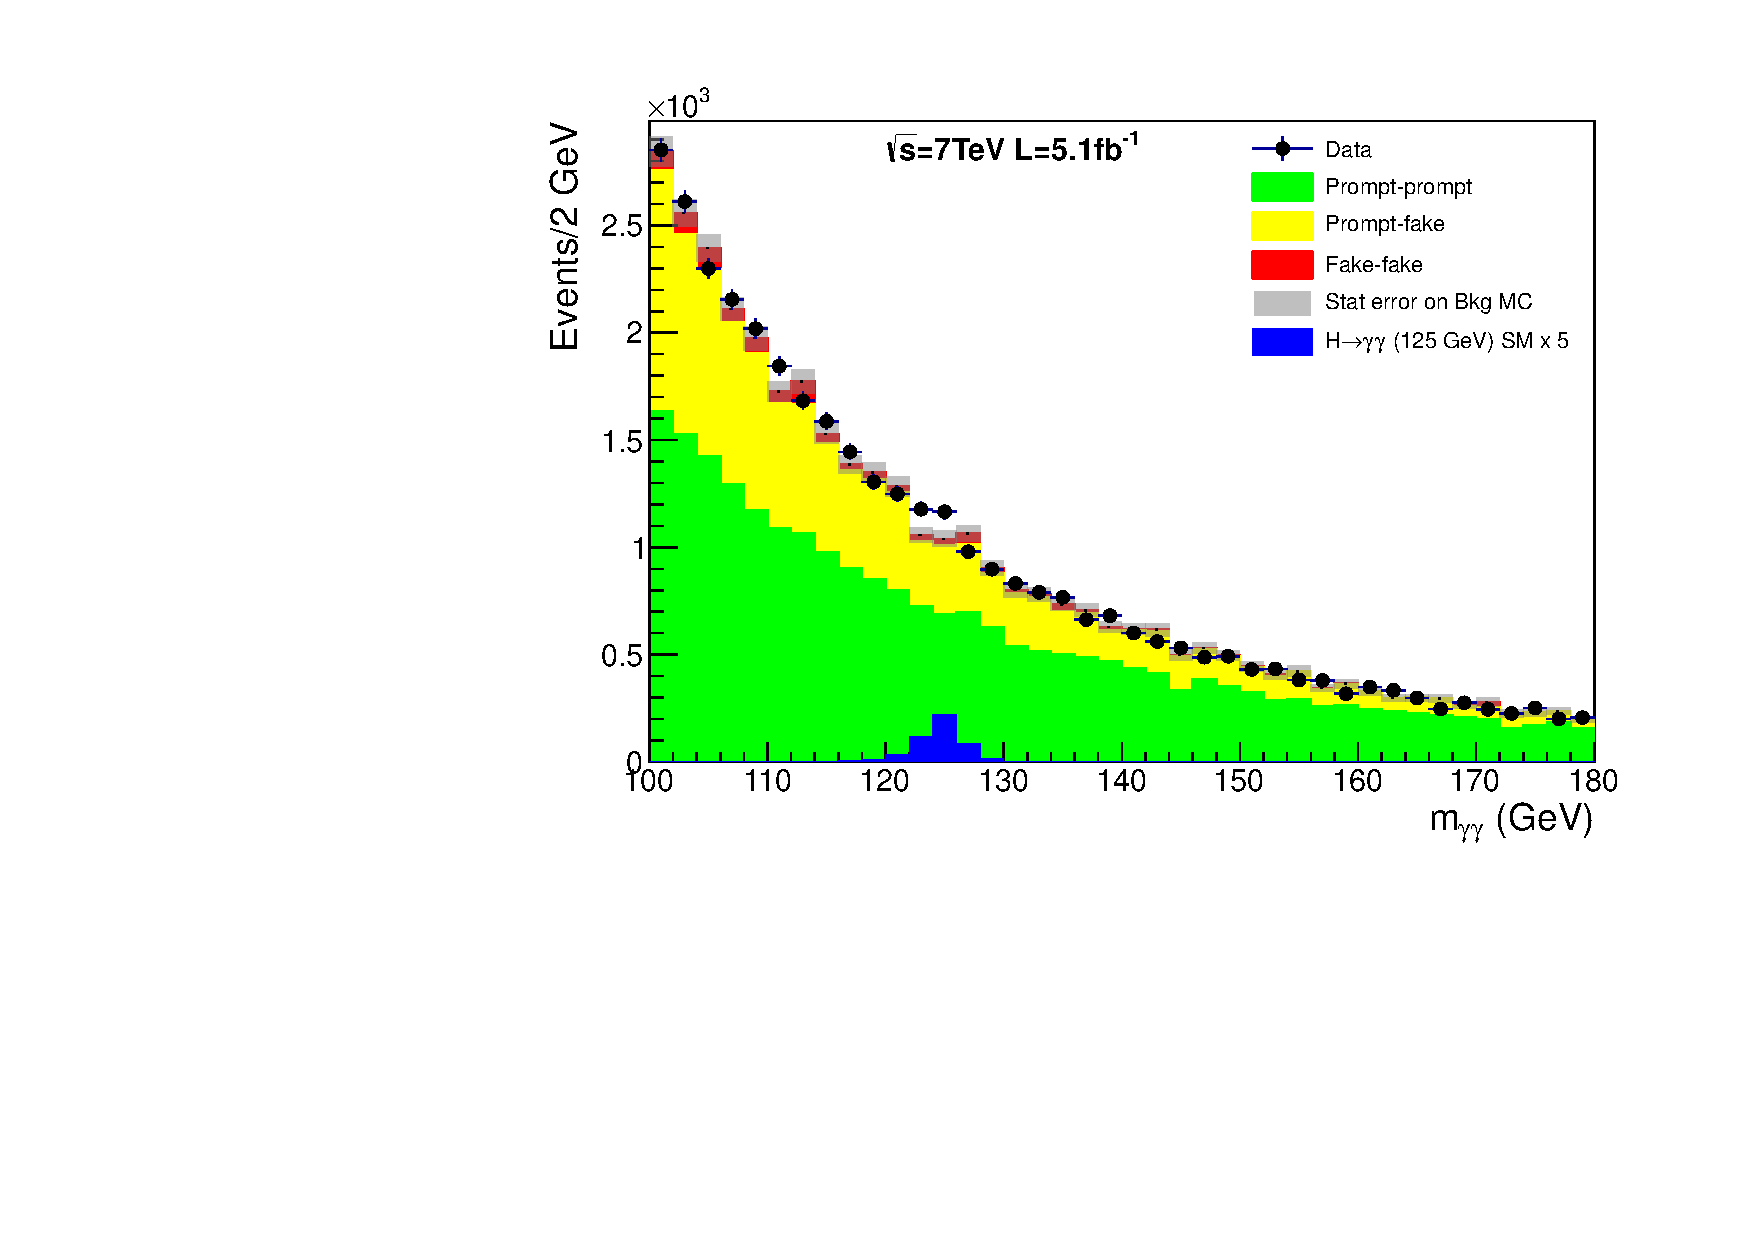
\includegraphics[width=0.48\textwidth]{analysis/plots/mgg_bkg_7TeV.pdf}
  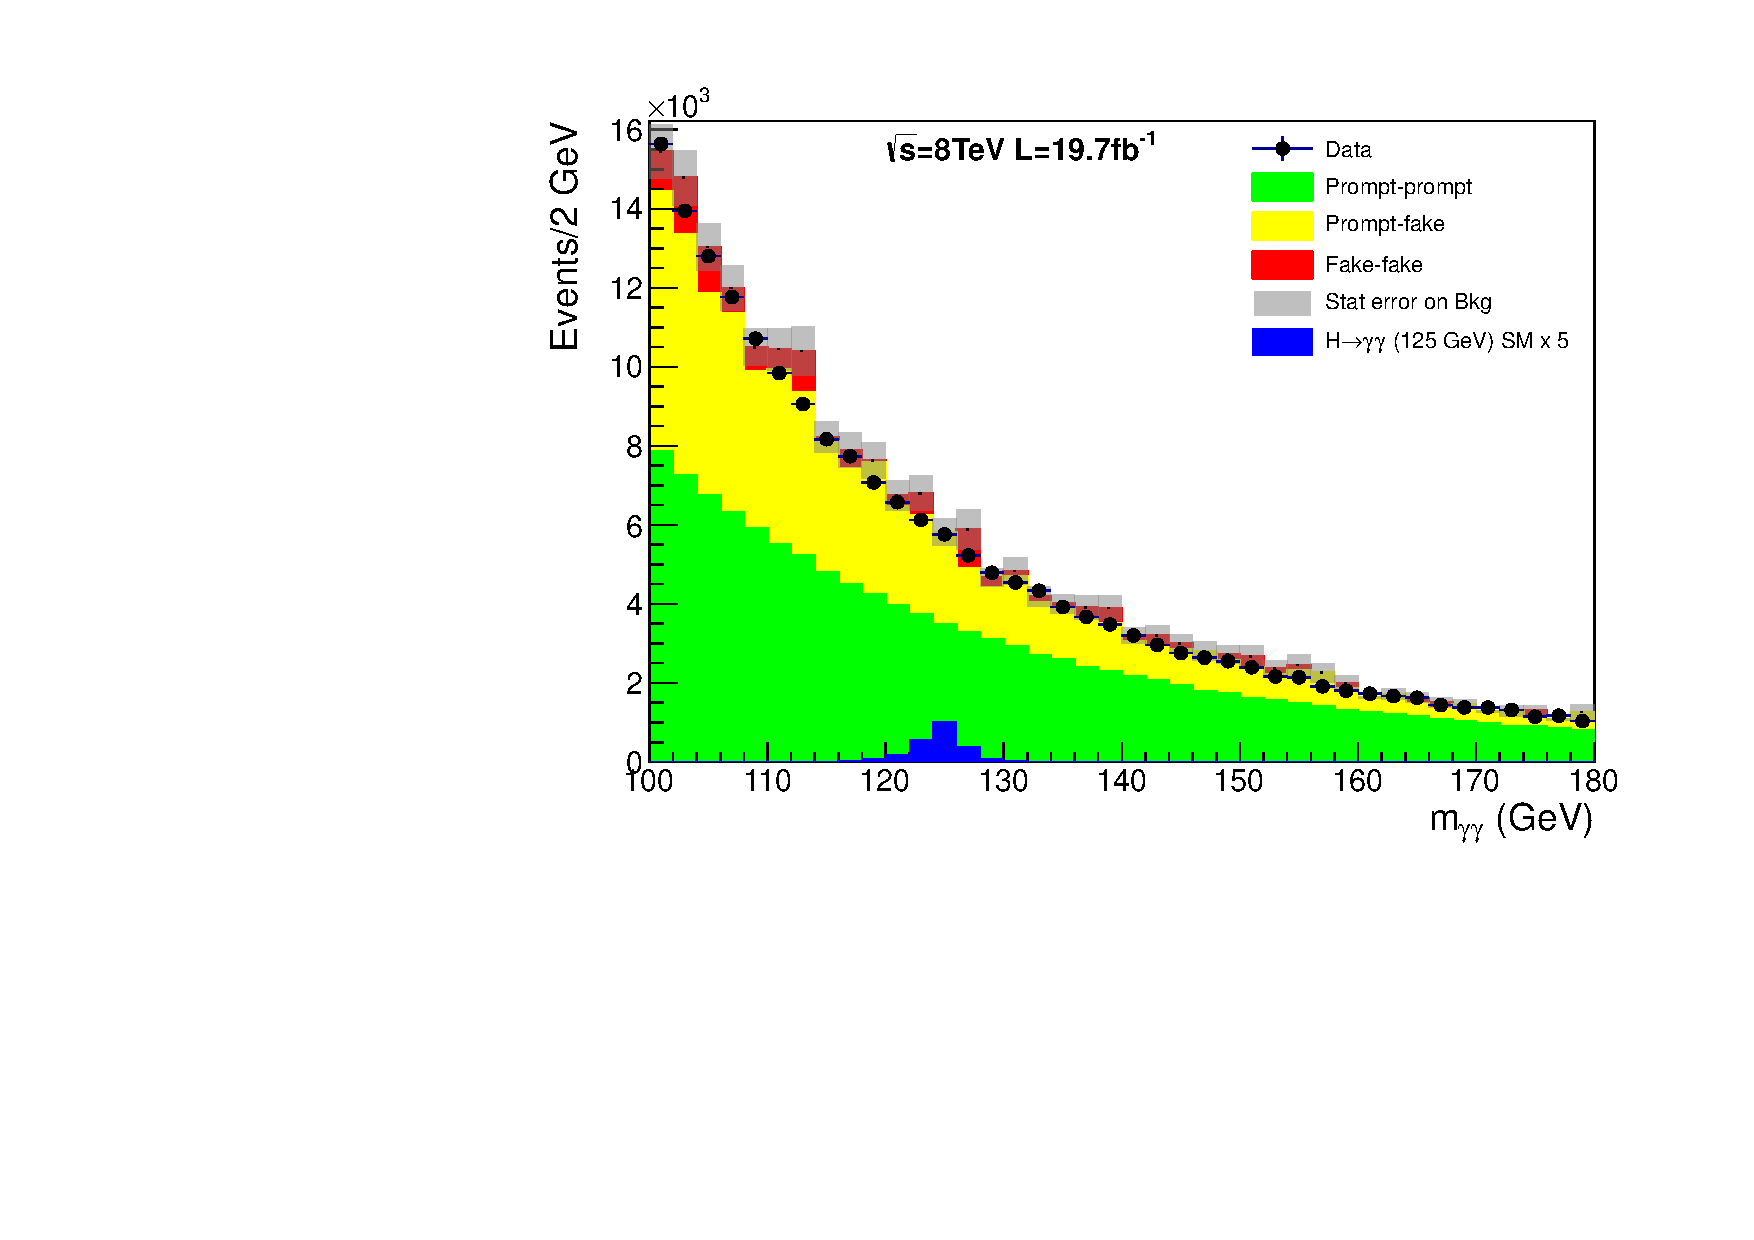
\includegraphics[width=0.48\textwidth]{analysis/plots/mgg_bkg_8TeV.pdf}
  \caption[Diphoton invariant mass distributions for the datasets at 7 and 8~TeV]{The diphoton invariant mass distribution for the 7 (left) and 8~TeV (right) dataets for the events which pass all of the analysis cuts. Cross-section weighted \MC events are plotted as the filled histograms for the prompt-prompt (green), prompt-fake (yellow) and fake-fake (red) backgrounds. The \SM signal expectation scaled up by a factor of 5 is shown by the blue histogram. The grey bands show the statistical uncertainty (sum of weights) of the background \MC events.}
  \label{fig:inv_mass_plots}
\end{figure}

% ---- SECTION ----
\section{Signal modelling}
\label{sec:signal_model}

The signal \MC samples (described in Sec.~\ref{sec:mc}) are propagated through the full analysis separately for each production mechanism (\ggH, \VBF, \WH, \ZH, \ttH). Events in the samples are weighted by the relevant \SM cross section, branching ratio, the integrated luminosity and the ``detector" weight which compensates for mismodelling in the \MC such as pileup, the beamspot width and discrepancies between the efficiency in data and \MC as measured in \Zee and \Zmumugamma decays. In this way the efficiency and acceptance of the detector, selection and categorisation is mapped by the \MC samples and the total number of expected \SM signal events is given by the sum of weights of the sample. The \MC is generated separately for hypothesised Higgs masses, \mH, in the search range of $110 \leq m_{H} \leq 150$~\GeV in steps of 5~\GeV. For any intermediate points the signal model is interpolated. The efficiency times acceptance of the analysis selection for a \SM Higgs boson is shown in Fig.~\ref{fig:effacc} as a function of the Higgs boson mass, \mH. For a Higgs at \mH=125~\GeV the $\ea=48.6\pm 0.7\%$ ($49.4\pm 0.7\%$) for the 7 (8)~\TeV datasets.

\begin{figure}
  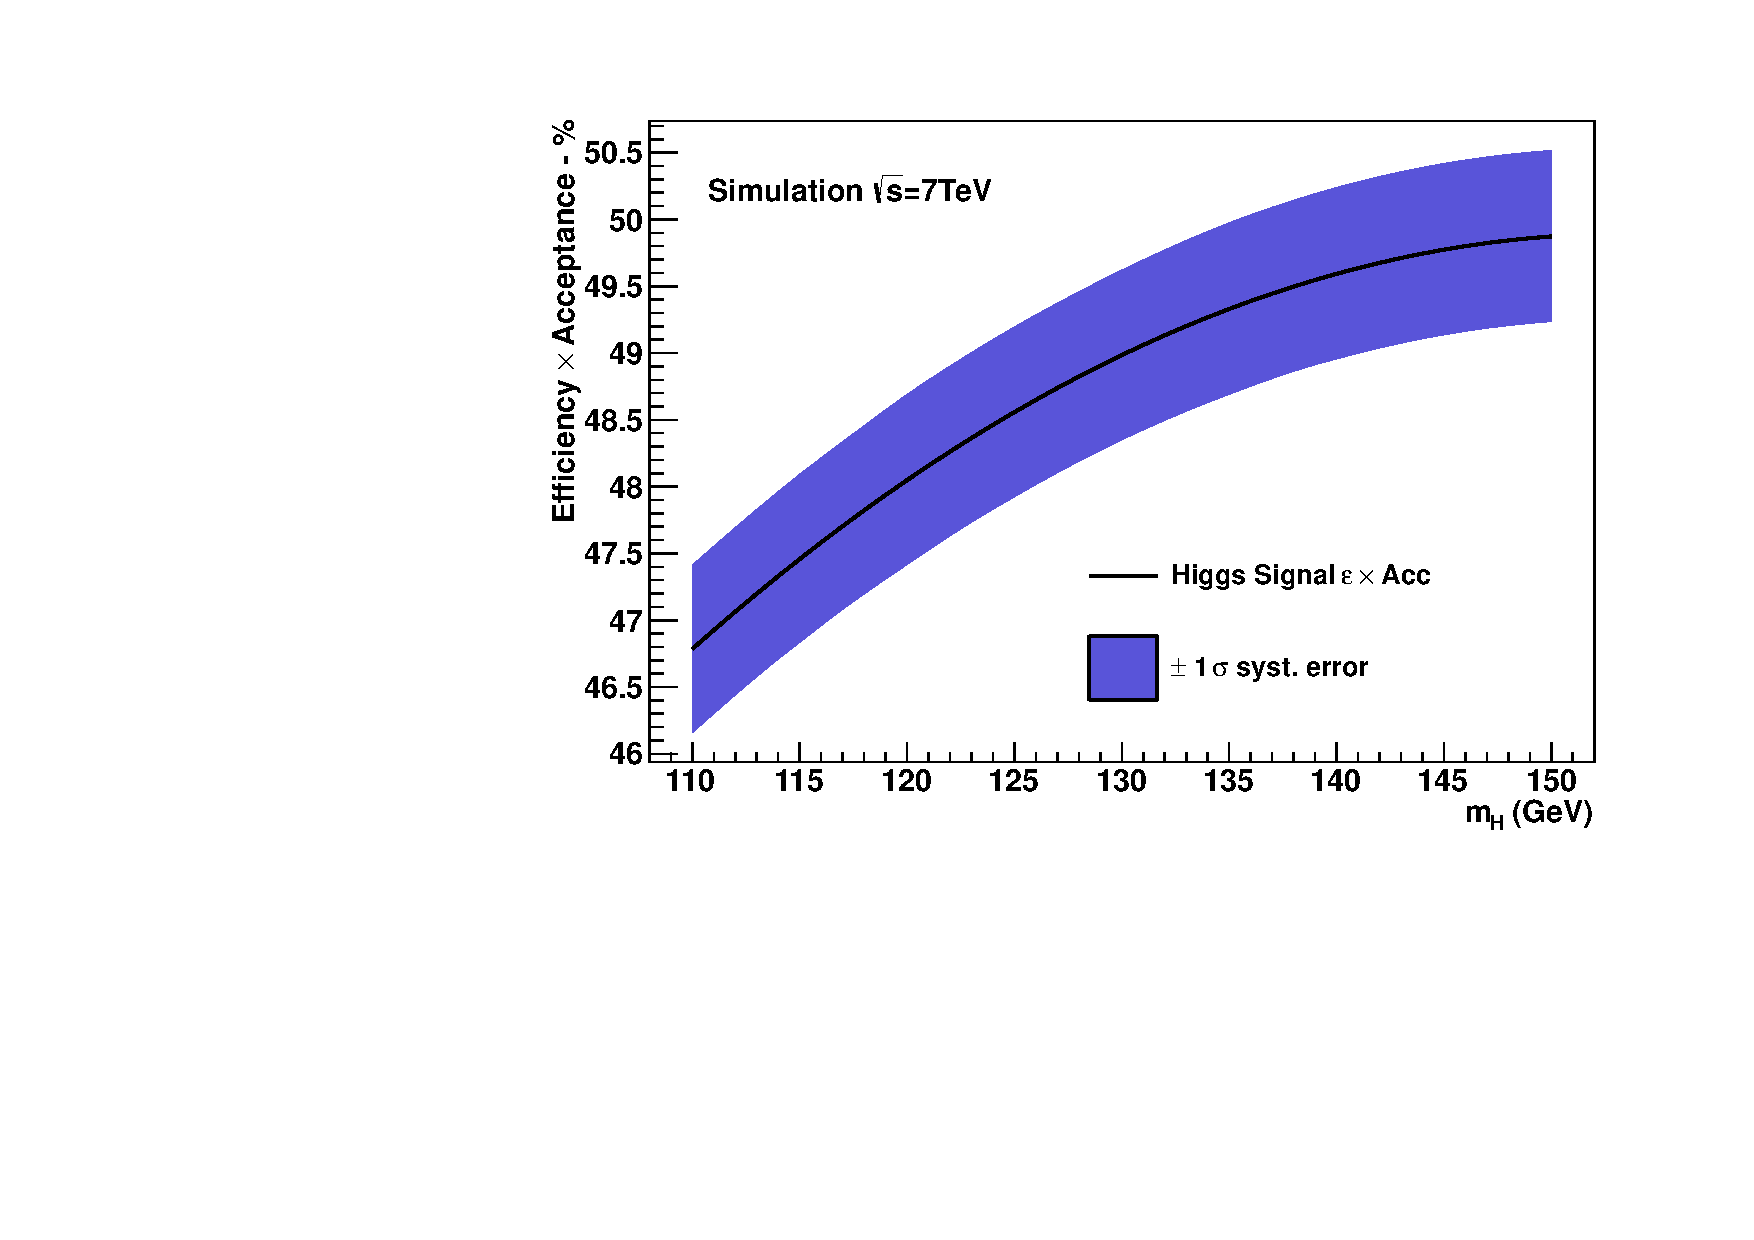
\includegraphics[width=0.49\textwidth]{analysis/plots/effAcc_vs_mass_7TeV.pdf}
  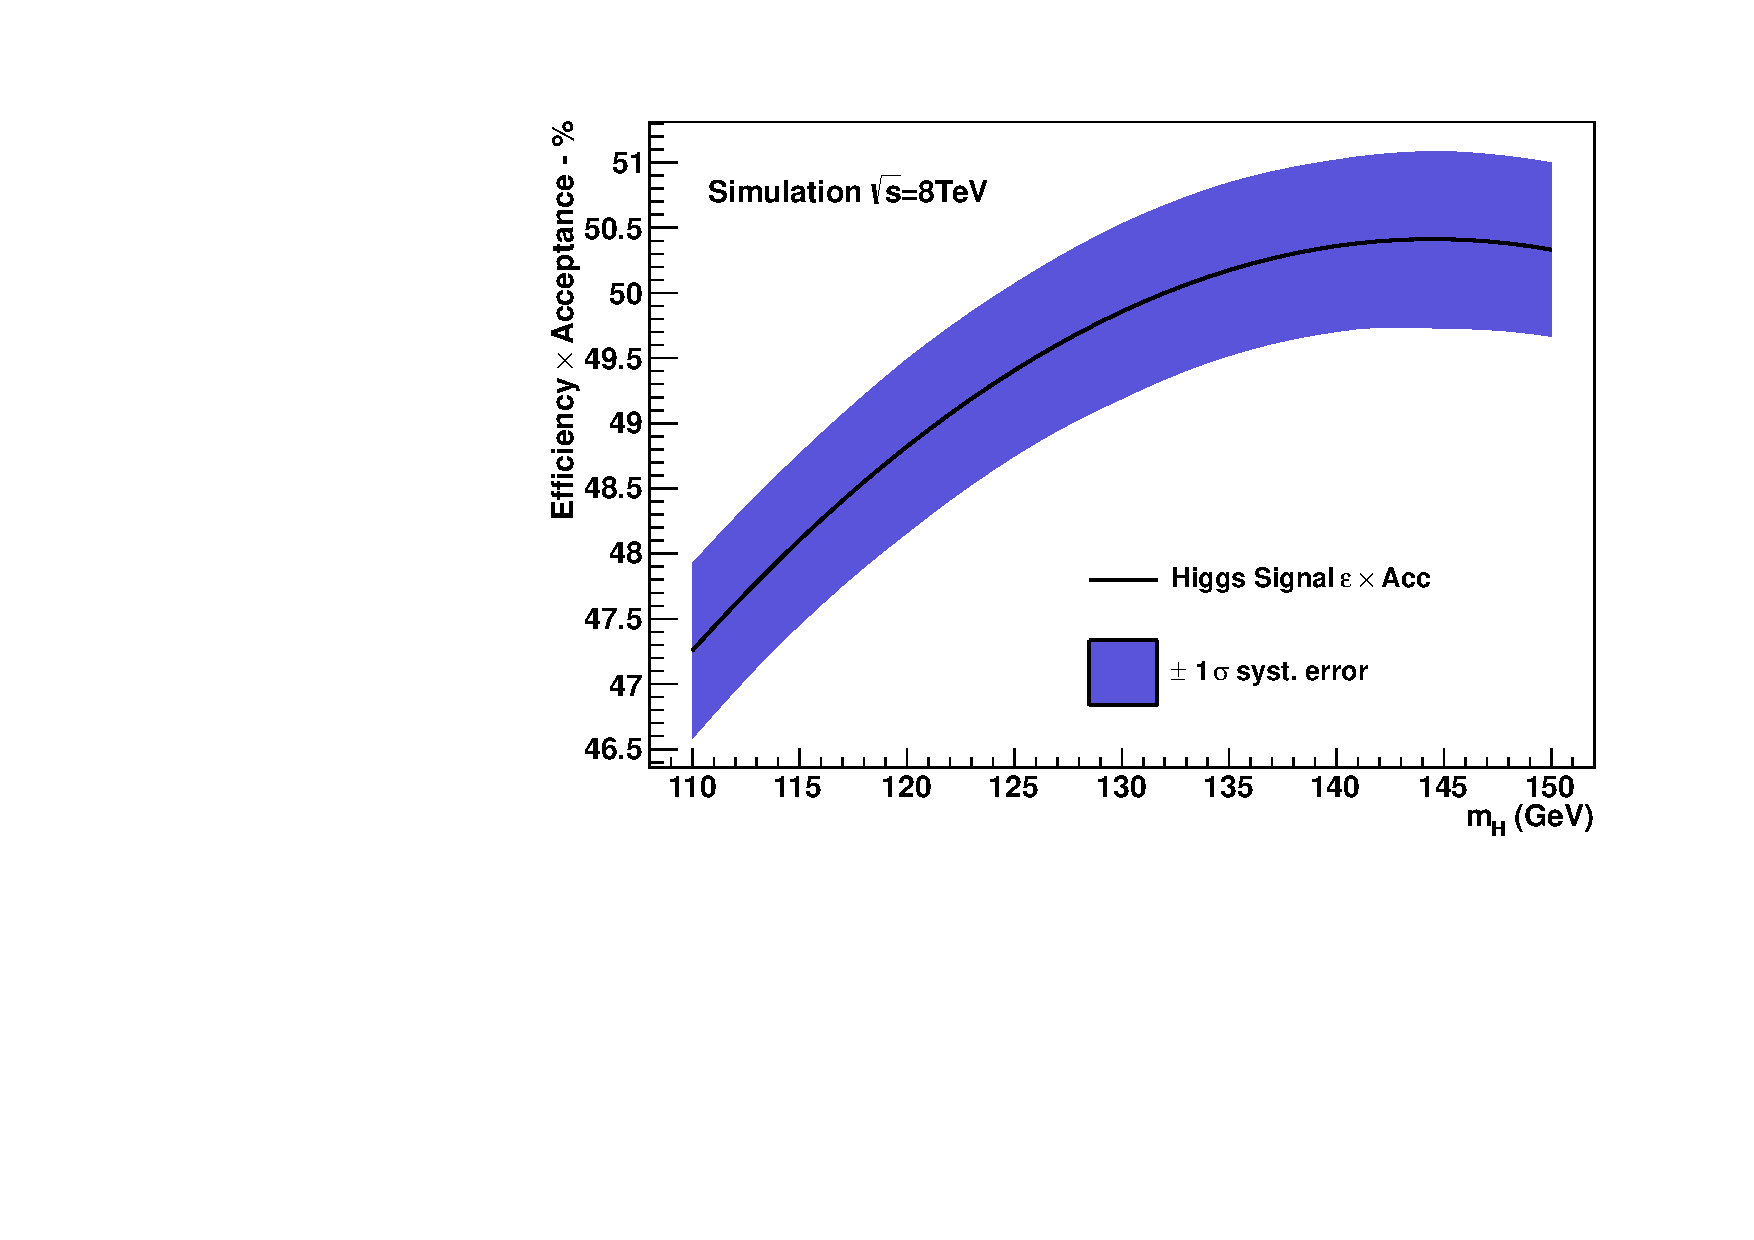
\includegraphics[width=0.49\textwidth]{analysis/plots/effAcc_vs_mass_8TeV.pdf}
  \caption[The efficiency$\times$acceptance of the analysis selection for \SM Higgs \MC]{The efficiency$\times$acceptance of the analysis selection for a \SM Higgs signal as a function of Higgs mass for the 7~\TeV (left) and 8~\TeV datasets.}
  \label{fig:effacc}
\end{figure}

\subsection{Mass factorised analysis}
\label{sec:signal_mfm}

The diphoton invariant mass signal shape is modelled in a fully parametric way for the \MFM. A separate model, consisting of a sum of Gaussians, is constructed for each production mechanism and each event class, where the two cases of right vertex and wrong (misidentified) vertex are fitted separately. The number of Gaussians used in the sum varies and can be as many as five although usually two or three provides an accurate description of the signal shape. A Gaussian sum is used because it has been found that this most accurately represents the shape of the invariant mass in signal. Many of the event classes contain a mixture of events from the resolution phase space (i.e.~there are mixtures of barrel/endcap and converted/unconverted photons) so by fitting with a sum of Gaussians these different components, which are in themselves Gaussian or close to Gaussian distributed, are accounted for. Some of the event classes for particular production mechanisms contain rather low \MC statistics (for example the lepton tagged category for signal produced by gluon fusion) and so fewer Gaussians are used in these cases. Clearly one expects a low signal yield for these particular cases and so a very accurate description of the shape is unnecessary. By allowing all the parameters in the Gaussian sums to float, including the means of the different Gaussian components, one obtains a parametrisation that models both the peak and tails of the signal distribution accurately. These fits are carried out at each value of \mH where signal \MC is available and then the individual fit parameters are linearly interpolated such that the shape is defined for any \mH in the range $[110,150]$~\GeV. The model therefore includes a floating parameter for the mass of the Higgs which can be fit to data. The right and wrong vertex shapes are then summed, with the relative fraction of right/wrong vertex events, to give a unique signal shape model in each event class for each production process. The signal normalisation, i.e.~the expected number of \SM signal events, is obtained by quadratically interpolating the efficiency $\times$ acceptance, \ea, for each event class and production process as calculated at the \mH points for which there is \MC. The total signal shape, summed over event classes and production mechanisms, is shown in Fig.~\ref{fig:sig_shape}. The total number of expected signal events, as well as the \sigeff (minimum interval containing 68.3\% of the distribution) and the \sigFW (full width at half the maximum divided by 2.35), for each event class are shown in Table~\ref{tab:sig_shape}. This information is additionally represented diagramatically in Fig.~\ref{fig:signal_composition} which provides an insightful summary of the analysis. The left hand column of this figure (Fig.~\ref{fig:signal_composition}) shows the breakdown of each signal process in each of the analysis categories. It can be seen that the \textit{untagged} categories contain mostly gluon fusion (green band) where the contribution of the other signal processes decreases when moving from ``Untagged 0" - ``Untagged 4". This is as we expect given that the signal processes which aren't gluon fusion produce Higgs bosons at higher \pT and thus get a higher diphoton \BDT score (see Fig.~\ref{fig:dipho_bdt}). A similar pattern can be seen for the dijet-tagged categories for which the signal consists of predominantly \VBF (red) but increasing amounts of \ggH (green) when moving from ``Dijet 0" - ``Dijet 2". Similarly the \VH-tagged categories consist of mainly \WH and \ZH signal (turqoiuse and blue) and the \ttH-tagged categories consists of mainly \ttH signal (orange). The middle column of this figure shows the signal model width (in terms of \sigeff and \sigFW) and demonstrates that categories which relate to a high score in the diphoton \BDT (``Untagged 0"/``Untagged 1") and a high score in the combined dijet-diphoton \BDT (``Dijet 0") are those with the best mass resolution. The right hand column of this figure shows the S/(S+B) ratio under the peak (within $\pm$\sigeff of \mH) and demonstrates the sensitivity of the individual categories.

\begin{figure}
  \begin{center}
    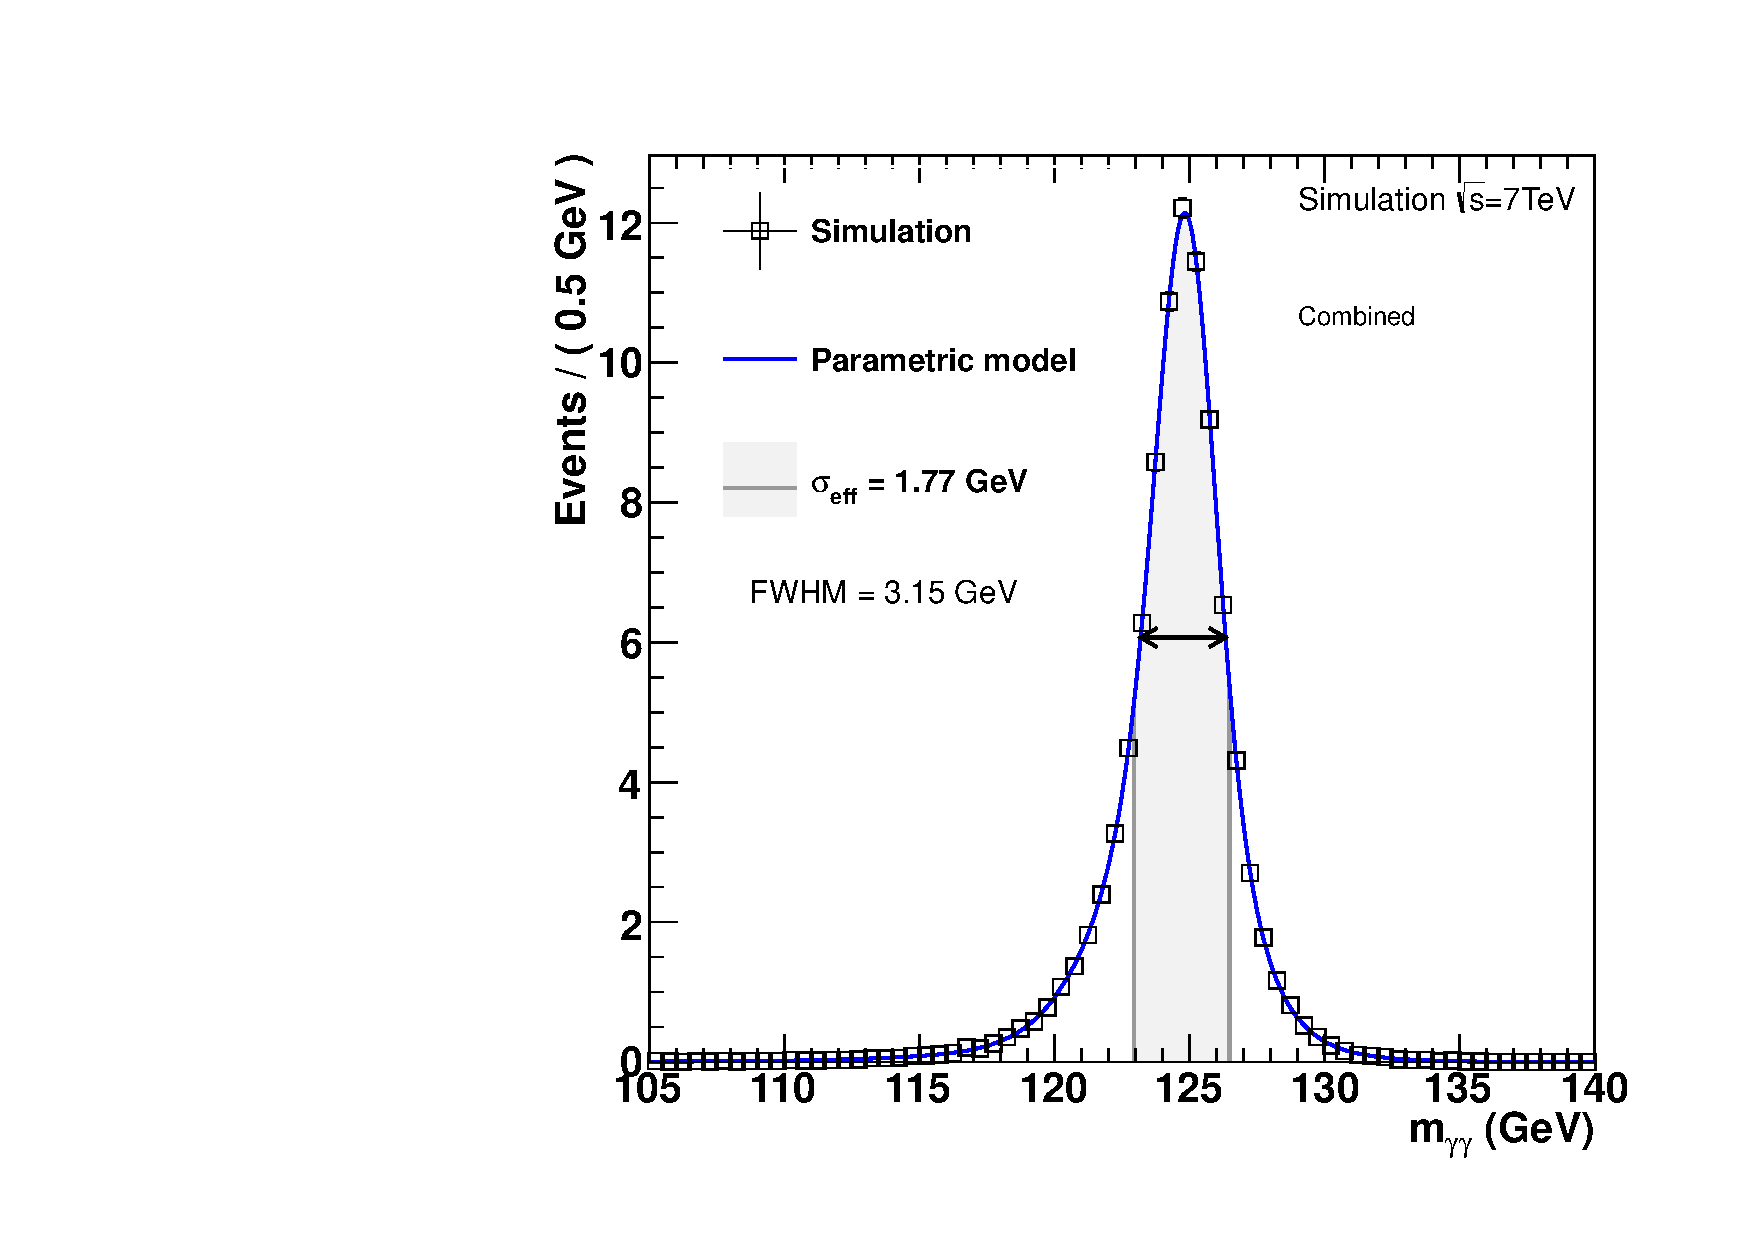
\includegraphics[width=0.49\textwidth]{analysis/plots/ThesisFits/mva_7TeV/all.pdf}
    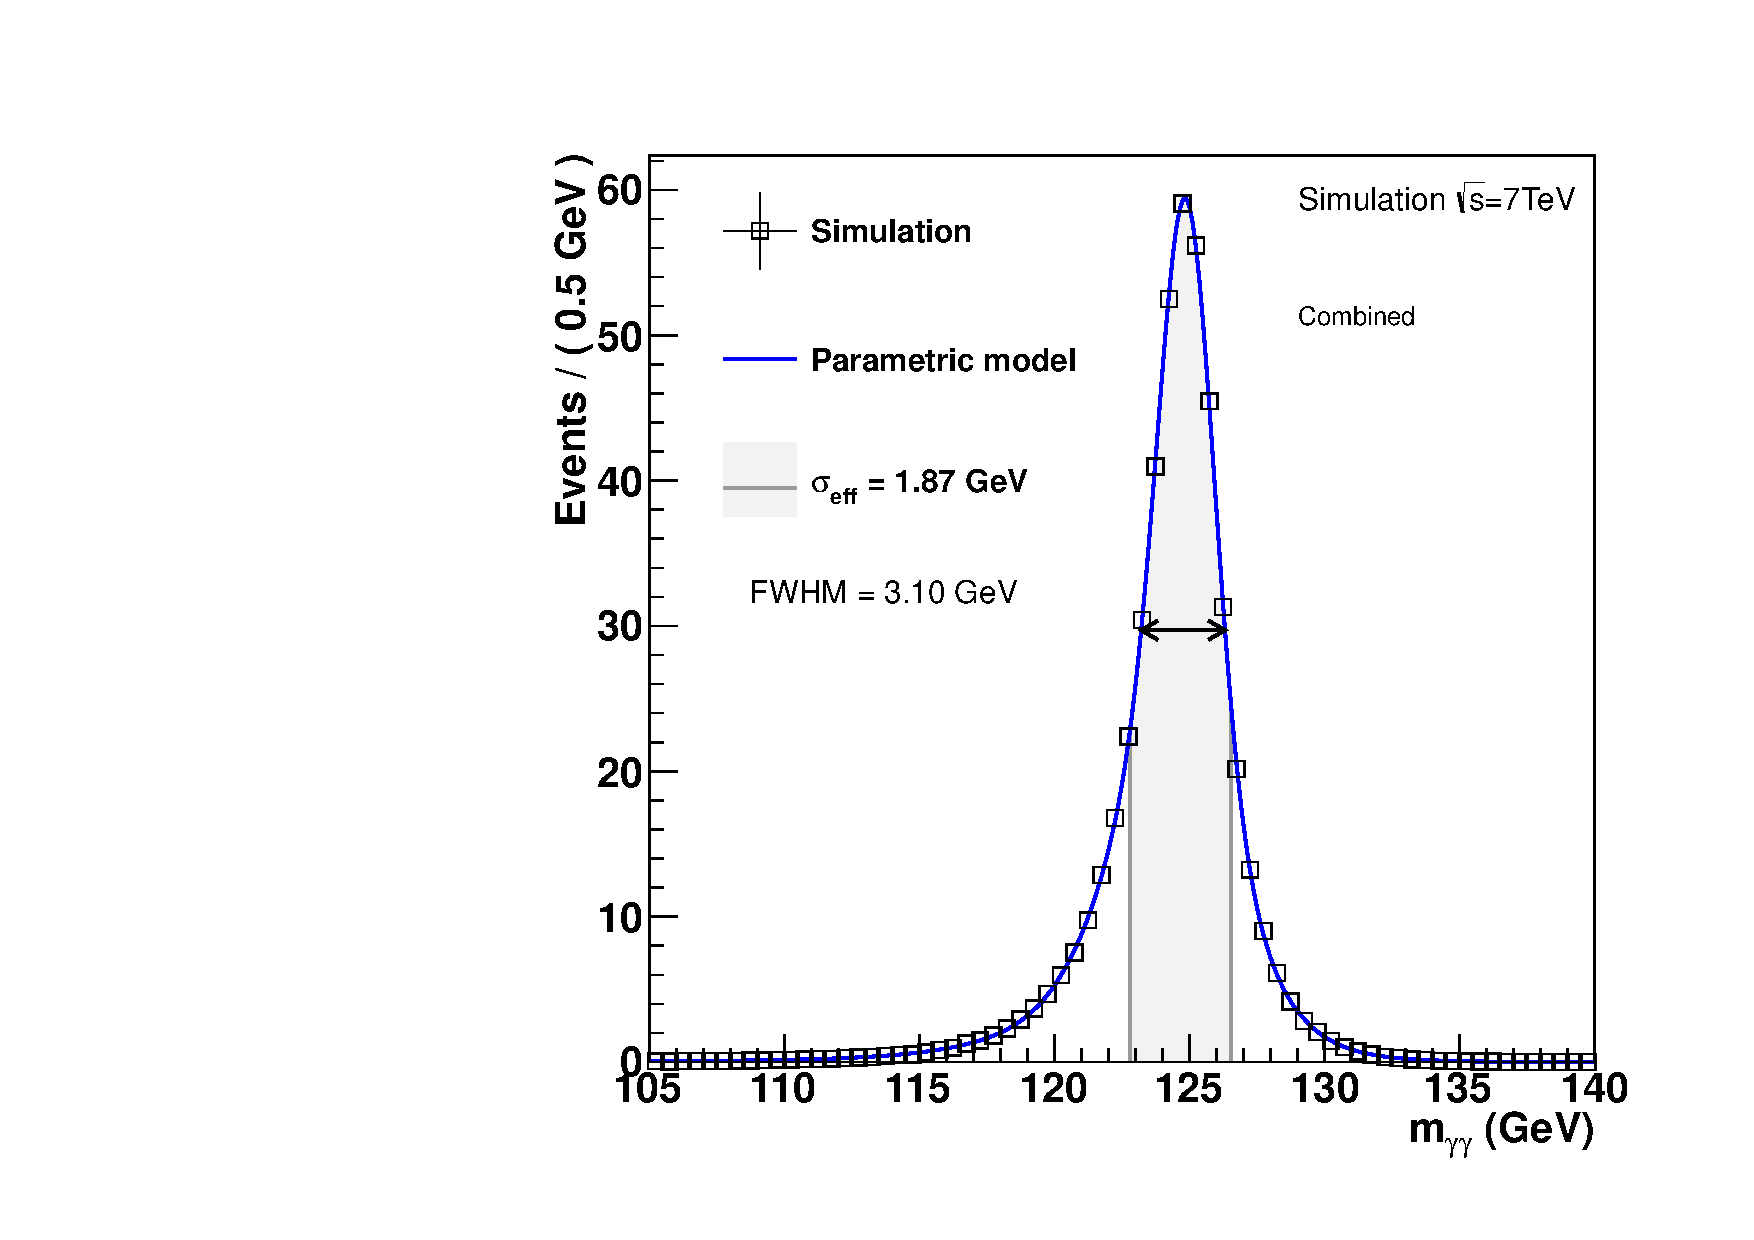
\includegraphics[width=0.49\textwidth]{analysis/plots/ThesisFits/mva_8TeV/all.pdf}
    \caption[The diphoton invariant mass shape for \SM Higgs signal]{The diphoton invariant mass shape of the \SM signal for the 7~\TeV dataset (left) and 8~\TeV dataset (right). The black square points show the distribution in \MC events, where the sum of weights represents the expected number of signal events from a \SM Higgs Boson at 125~\GeV. The blue line shows the shape of the parametric model used to represent the signal.}
    \label{fig:sig_shape}
  \end{center}
\end{figure}

\begin{table}[htbp]
\begin{center}
\caption{Expected number of SM Higgs boson events ($\mH=125\GeV$) and
estimated background (``Bkg.'') at $\mgg=125\GeV$ for all event classes of the 7
and 8\TeV datasets.
The composition of the SM Higgs boson signal in terms of the production
processes and its mass resolution is also given.
Numbers are omitted for production processes contributing less than 0.05\% to the signal.}
\resizebox{\columnwidth}{!}{%%%% ---- beginning of resize
\begin{tabular}{|c|r|r|rrrrr|c|c|r|}
\hline                                                                                                                                          
\multicolumn{2}{|c|}{\multirow{3}{*}{Event classes}} & \multicolumn{8}{c|}{SM Higgs boson expected signal (\mH=125\GeV)} & \multicolumn{1}{c|}{Bkg.} \\
\cline{3-10}
\multicolumn{2}{|c|}{} & \multirow{2}{*}{Total} & \multirow{2}{*}{ggH} & \multirow{2}{*}{VBF} & \multirow{2}{*}{WH} & \multirow{2}{*}{ZH} & \multirow{2}{*}{\ttH} & $\sigma_\mathrm{eff}$ & $\sigma_\mathrm{FW}$ & \multicolumn{1}{c|}{\footnotesize{($\text{GeV}^{-1}$)}} \\
\multicolumn{2}{|c|}{} & & & & & & & \footnotesize{(GeV)} & \footnotesize{(GeV)} &  \\
\hline
\multirow{11}{*}{\begin{sideways}{7\TeV 5.1fb$^{-1}$}\end{sideways}}
& Untagged 0 & 5.8 & 79.8\% & 9.9\% & 6.0\% & 3.5\% & 0.8\% & 1.11 & 0.98 & 11.0 \\ 
& Untagged 1 & 22.7 & 91.9\% & 4.2\% & 2.4\% & 1.3\% & 0.2\% & 1.27 & 1.09 & 69.5 \\ 
& Untagged 2 & 27.1 & 91.9\% & 4.1\% & 2.4\% & 1.4\% & 0.2\% & 1.78 & 1.40 & 134.6 \\ 
& Untagged 3 & 34.1 & 92.1\% & 4.0\% & 2.4\% & 1.3\% & 0.2\% & 2.36 & 2.01 & 311.9 \\ 
\cline{2-11}
& VBF dijet 0 & 1.6 & 19.3\% & 80.1\% & 0.3\% & 0.2\% & 0.1\% & 1.41 & 1.17 & 0.5 \\ 
& VBF dijet 1 & 3.0 & 38.1\% & 59.5\% & 1.2\% & 0.7\% & 0.4\% & 1.65 & 1.32 & 3.5 \\ 
\cline{2-11}
& VH tight $\ell$ & 0.3 & ---~~ & ---~~ & 77.2\% & 20.6\% & 2.2\% & 1.61 & 1.31 & 0.1 \\ 
& VH loose $\ell$ & 0.2 & 3.6\% & 1.1\% & 79.1\% & 15.2\% & 1.0\% & 1.63 & 1.32 & 0.2 \\ 
& VH \MET & 0.3 & 4.5\% & 1.1\% & 41.5\% & 44.6\% & 8.2\% & 1.60 & 1.14 & 0.2 \\ 
& VH dijet & 0.4 & 27.1\% & 2.8\% & 43.7\% & 24.3\% & 2.1\% & 1.54 & 1.24 & 0.5 \\ 
\cline{2-11}
& \ttH tags & 0.2 & 3.1\% & 1.1\% & 2.2\% & 1.3\% & 92.3\% & 1.40 & 1.13 & 0.2 \\ 
\hline
\noalign{\vskip 1mm}
\hline
\multirow{14}{*}{\begin{sideways}{8\TeV 19.7fb$^{-1}$}\end{sideways}}
& Untagged 0 & 6.0 & 75.7\% & 11.9\% & 6.9\% & 3.6\% & 1.9\% & 1.05 & 0.79 & 4.7 \\ 
& Untagged 1 & 50.8 & 85.2\% & 7.9\% & 4.0\% & 2.4\% & 0.6\% & 1.19 & 1.00 & 119.6 \\ 
& Untagged 2 & 117.2 & 91.1\% & 4.7\% & 2.5\% & 1.4\% & 0.3\% & 1.46 & 1.15 & 418.2 \\ 
& Untagged 3 & 153.1 & 91.6\% & 4.4\% & 2.4\% & 1.4\% & 0.3\% & 2.04 & 1.56 & 870.3 \\ 
& Untagged 4 & 121.4 & 93.1\% & 3.6\% & 2.0\% & 1.1\% & 0.2\% & 2.62 & 2.14 & 1401.3 \\ 
\cline{2-11}
& VBF dijet 0 & 4.5 & 17.8\% & 81.8\% & 0.2\% & 0.1\% & 0.1\% & 1.30 & 0.94 & 0.8 \\ 
& VBF dijet 1 & 5.6 & 28.5\% & 70.5\% & 0.6\% & 0.2\% & 0.2\% & 1.43 & 1.07 & 2.7 \\ 
& VBF dijet 2 & 13.7 & 43.8\% & 53.2\% & 1.4\% & 0.8\% & 0.8\% & 1.59 & 1.24 & 22.1 \\ 
\cline{2-11}
& VH tight $\ell$ & 1.4 & 0.2\% & 0.2\% & 76.9\% & 19.0\% & 3.7\% & 1.63 & 1.24 & 0.4 \\ 
& VH loose $\ell$ & 0.9 & 2.6\% & 1.1\% & 77.9\% & 16.8\% & 1.5\% & 1.60 & 1.16 & 1.2 \\ 
& VH \MET & 1.8 & 16.3\% & 2.7\% & 34.4\% & 35.4\% & 11.1\% & 1.68 & 1.17 & 1.3 \\ 
& VH dijet & 1.6 & 30.3\% & 3.1\% & 40.6\% & 23.4\% & 2.6\% & 1.31 & 1.06 & 1.0 \\ 
\cline{2-11}
& \ttH lepton & 0.5 & ---~~ & ---~~ & 1.6\% & 1.6\% & 96.8\% & 1.34 & 1.03 & 0.2 \\ 
& \ttH multijet & 0.6 & 4.1\% & 0.9\% & 0.8\% & 0.9\% & 93.3\% & 1.34 & 1.03 & 0.6 \\ 
\hline
\end{tabular}
}%%%% ---- end of resize

\label{tab:sig_shape}
\end{center} 
\end{table}


                                                                                                             

  
\begin{figure}
  \begin{center}
    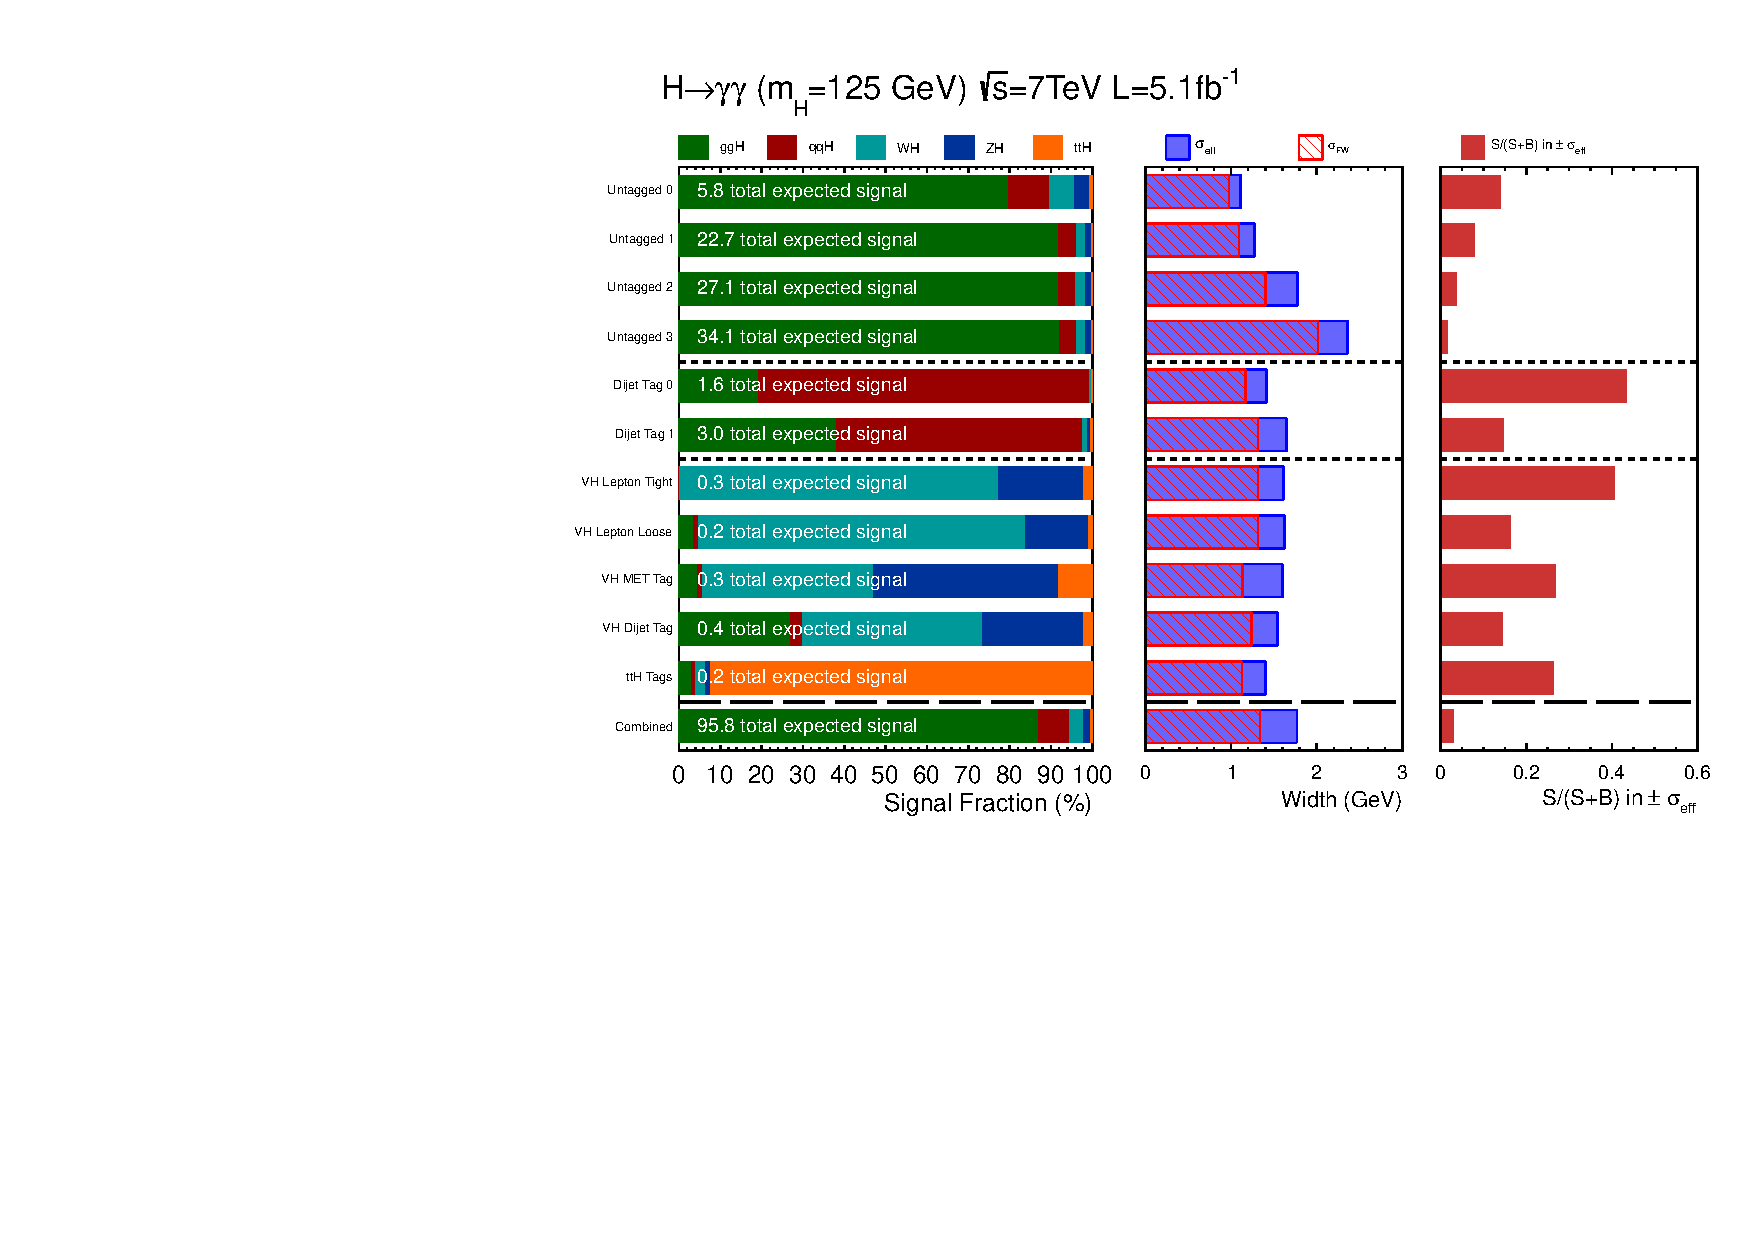
\includegraphics[width=0.9\textwidth]{analysis/plots/ThesisFits/mva_7TeV/signalComposition_fix.pdf} \\
    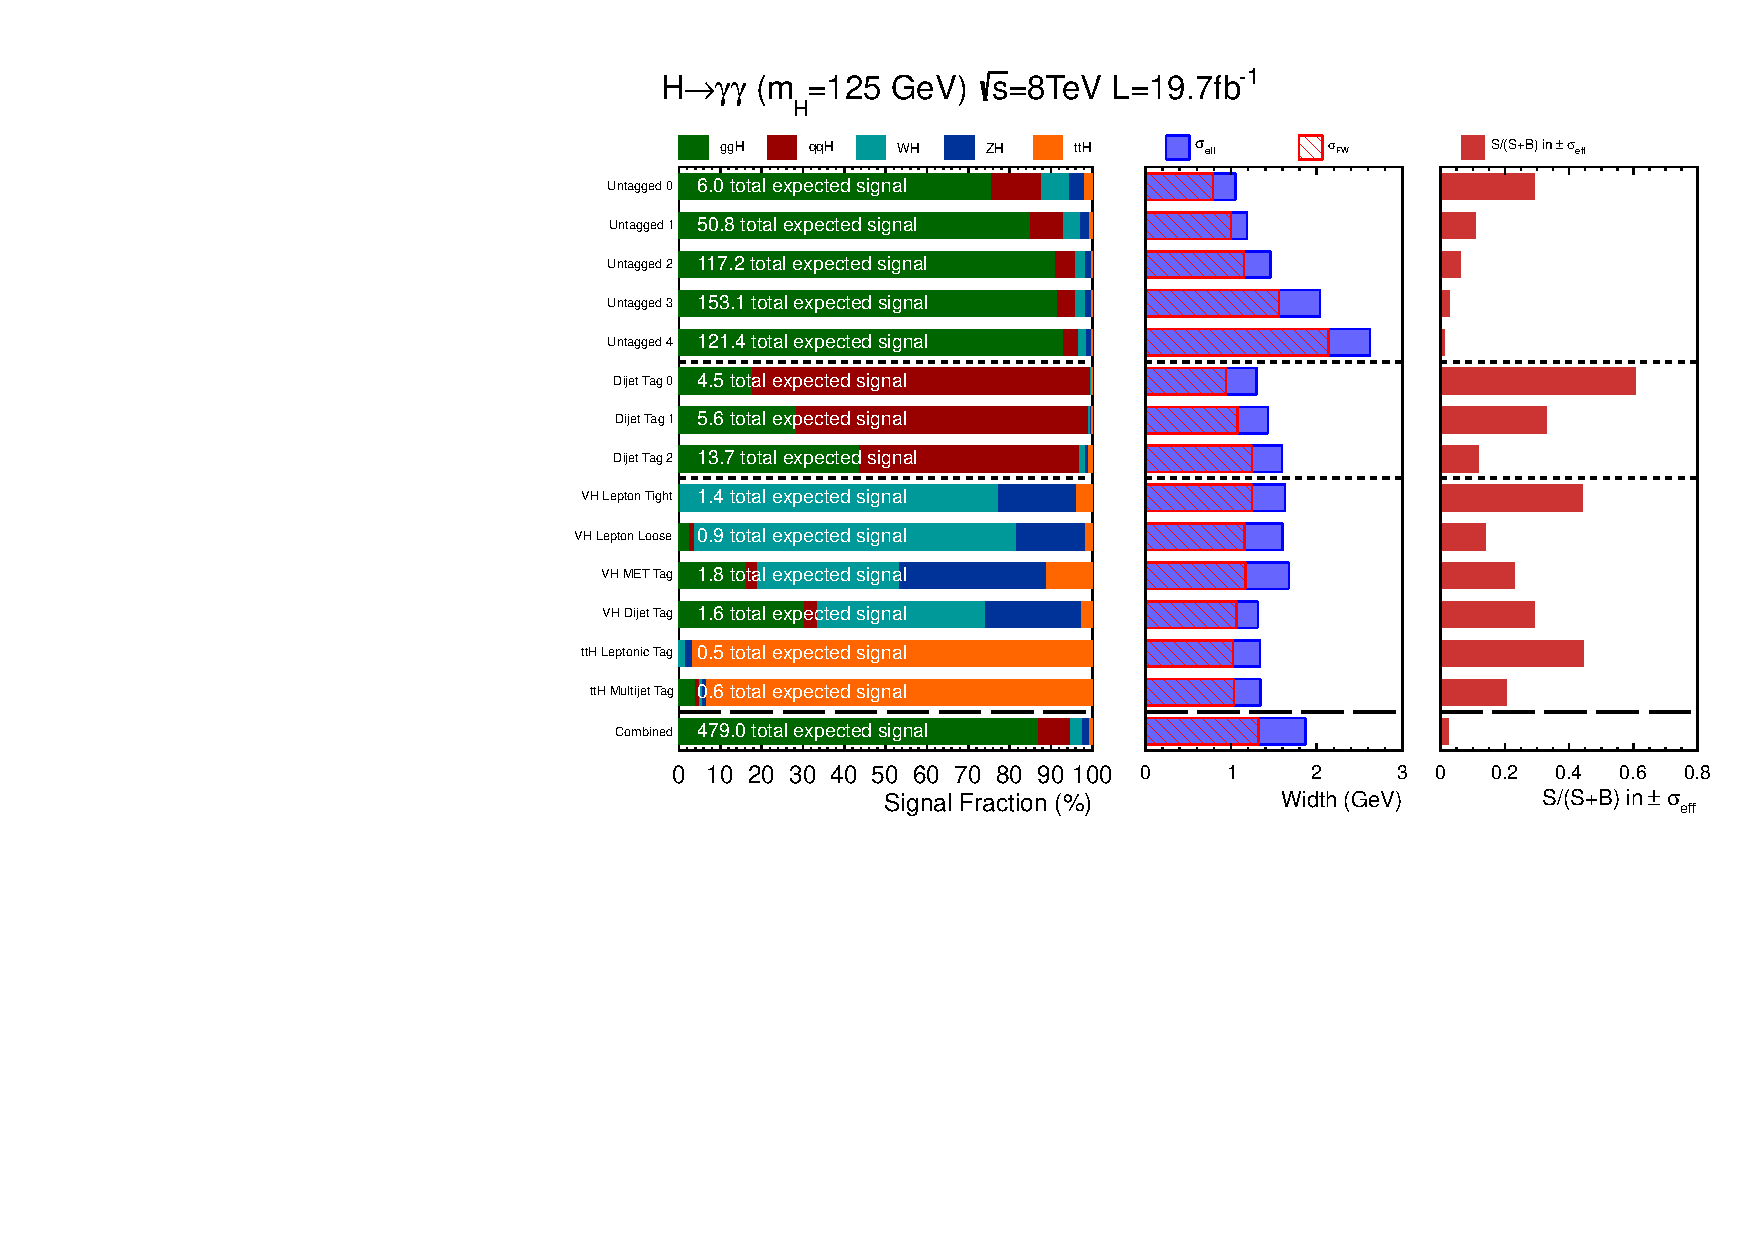
\includegraphics[width=0.9\textwidth]{analysis/plots/ThesisFits/mva_8TeV/signalComposition_fix.pdf}
    \caption[The composition and width of the signal in each analysis category]{The expected composition and resolution of the signal for a \SM Higgs at 125~\GeV in the 7~\TeV dataset (top) and 8~\TeV dataset (bottom). The left diagram shows the breakdown of the signal in each event class by category: \ggH (green), \VBF (red), \WH (turqoise), \ZH (blue), \ttH (orange). The middle diagram shows the expected resolution in each event class in terms of \sigeff and \sigFW. The right diagram shows the expected signal over signal-plus-background ratio in a window of $\pm\sigeff$ around \mH=125~\GeV.}
    \label{fig:signal_composition}
  \end{center}
\end{figure}
  
\subsection{Sideband analysis}
\label{sec:sig_sideband}

The signal model shape is mapped by the categorisation scheme described in Sec.~\ref{sec:inclusive_cats_sideband} whereby events nearer the signal peak are collected in bins with higher sensitivity (see Fig.~\ref{fig:sideband_cats}). The statistical method used for the sideband method is not a parametric shape analysis like the \MFM but implemented as a simple counting experiment, across the analysis bins, inside the signal region, which is defined as a $\pm$2\% window around the hypothesised Higgs mass, \mH. This is simply the sum of weights of the \MC samples in each analysis bin inside the window for values of \mH for which there exists \MC samples. The signal shape, i.e.~the signal distribution in the analysis bins, is linearly interpolated for any intermediate values of \mH. As for the \MFM the \SM production mechanisms are propagated through the analysis separately. The signal normalization at each Higgs mass is calculated in a similar way as for the \MFM in which the \ea is linearly interpolated between the masses at which there are \MC samples and then scaled by cross section, branching ratio and integrated luminosity. 

% ---- SECTION ----
\section{Background modelling}
\label{sec:background_model}

The background is the most significant unknown in this analysis. The size of the background relative to the signal is large and the invariant mass shape of the backgroud is poorly modelled in \MC. It is known to be a smoothly varying and falling spectrum, however various detector effects such as reconstruction, energy resolution and triggering which are imperfectly modelled in the \MC can distort the shape. Furthermore the contribution of fake photons to the background varies as a function of \mgg and this is not well modelled in the theory or detector simulation. One of the main motivations for having the two analyses described here is that they have completely different ways of measuring the background and consequently serve to cross check each other. Both analyses use entirely data-driven methods for extracting the background.  

\subsection{Mass factorised analysis}
\label{sec:envelope}

A unique and novel way of estimating the background, given we have no \emph{a priori} knowledge of its shape, has been developed specifically for this analysis. The method, laterly referred to as the ``envelope" method, attempts to parametrise our ignorance of the background shape in a similar way to what is done for normal nuisance parameters when using the negative log likelihood to obtain the best fit value of a quantity and its error using frequentist statistical methods~\cite{FredJames}. To explain better the method let us first consider the simplified case of fitting a probability distribution to a dataset where the probability distribution contains one physical \POI, $x$, (which could for example represent the signal mass) and one nuisance parameter, $\theta$, (which could represent the energy scale uncertainty). In this case we can calculate twice the negative log likelihood, $-2$LL, at different values of $x$ whilst at each point minimising the likelihood with respect to \theta. 
This would give us the best fit value of $x$ and its error given the variation allowed by \theta. This is represented in Fig.~\ref{fig:envelope_explain1} by the solid black line. The best fit value of $x$ is given at the minimum of the likelihood and the 1$\sigma$ error interval defined as the range where twice the negative log likelood relative to the global minimum (best fit value) is less than one, \NLL$\leq1$. This is known as the ``profile likelihood method" as the nuisance parameter, $\theta$, is ``profiled" (i.e.\ floated) in the fit. In other words, for a given value of $x$ the value of $\theta$ which minimizes the likelihood is chosen. One can redo the likelihood scan fixing $\theta$ to its value at the best fit and this gives a narrower likelihood curve, demonstrated by the solid blue line in Fig.~\ref{fig:envelope_explain1}. In this case the error, the range for which \NLL$\leq1$, is smaller as one would expect given the nuisance parameter is now frozen. This is equivalent to the statistical error only, as the systematic component parametrised by $\theta$ is ignored. One can now also build up a multitude of curves by setting the nuisance parameter $\theta$ to arbitary values and rescanning the likelihood, these are shown in Fig.~\ref{fig:envelope_explain1} as the red dashed lines. It should be clear that by taking the ``envelope" around the potentially infinite set of red curves one can reproduce the black line representing the full profile fit providing the full $\theta$ phase space is sampled enough times. 
This is shown in the figure by the magenta line which becomes smoother as more sets of $\theta$ values are chosen. It is worth noting that not all of the red curves (of which there are infinitely many) necessarily have to touch the black line: a very extreme value of $\theta$ will give a bad fit and the corresponding red dashed curve would be off the plot. In this way one could in principal ``reverse-engineer" the profile likelihood method such that the profiling of the nuisance parameter $\theta$ is not done as a continuous minimisation but as a series of discrete minimisations, where the minimum \NLL for a given value of $x$ is taken as the minimum \NLL over all discrete choices of $\theta$ at this value of $x$. Clearly, for a case in which the nuisance parameter $\theta$ is continous this is inefficient and unnecessary but it is effective if the nuisance parameter can only take discrete values.

\begin{figure}
\begin{center}
  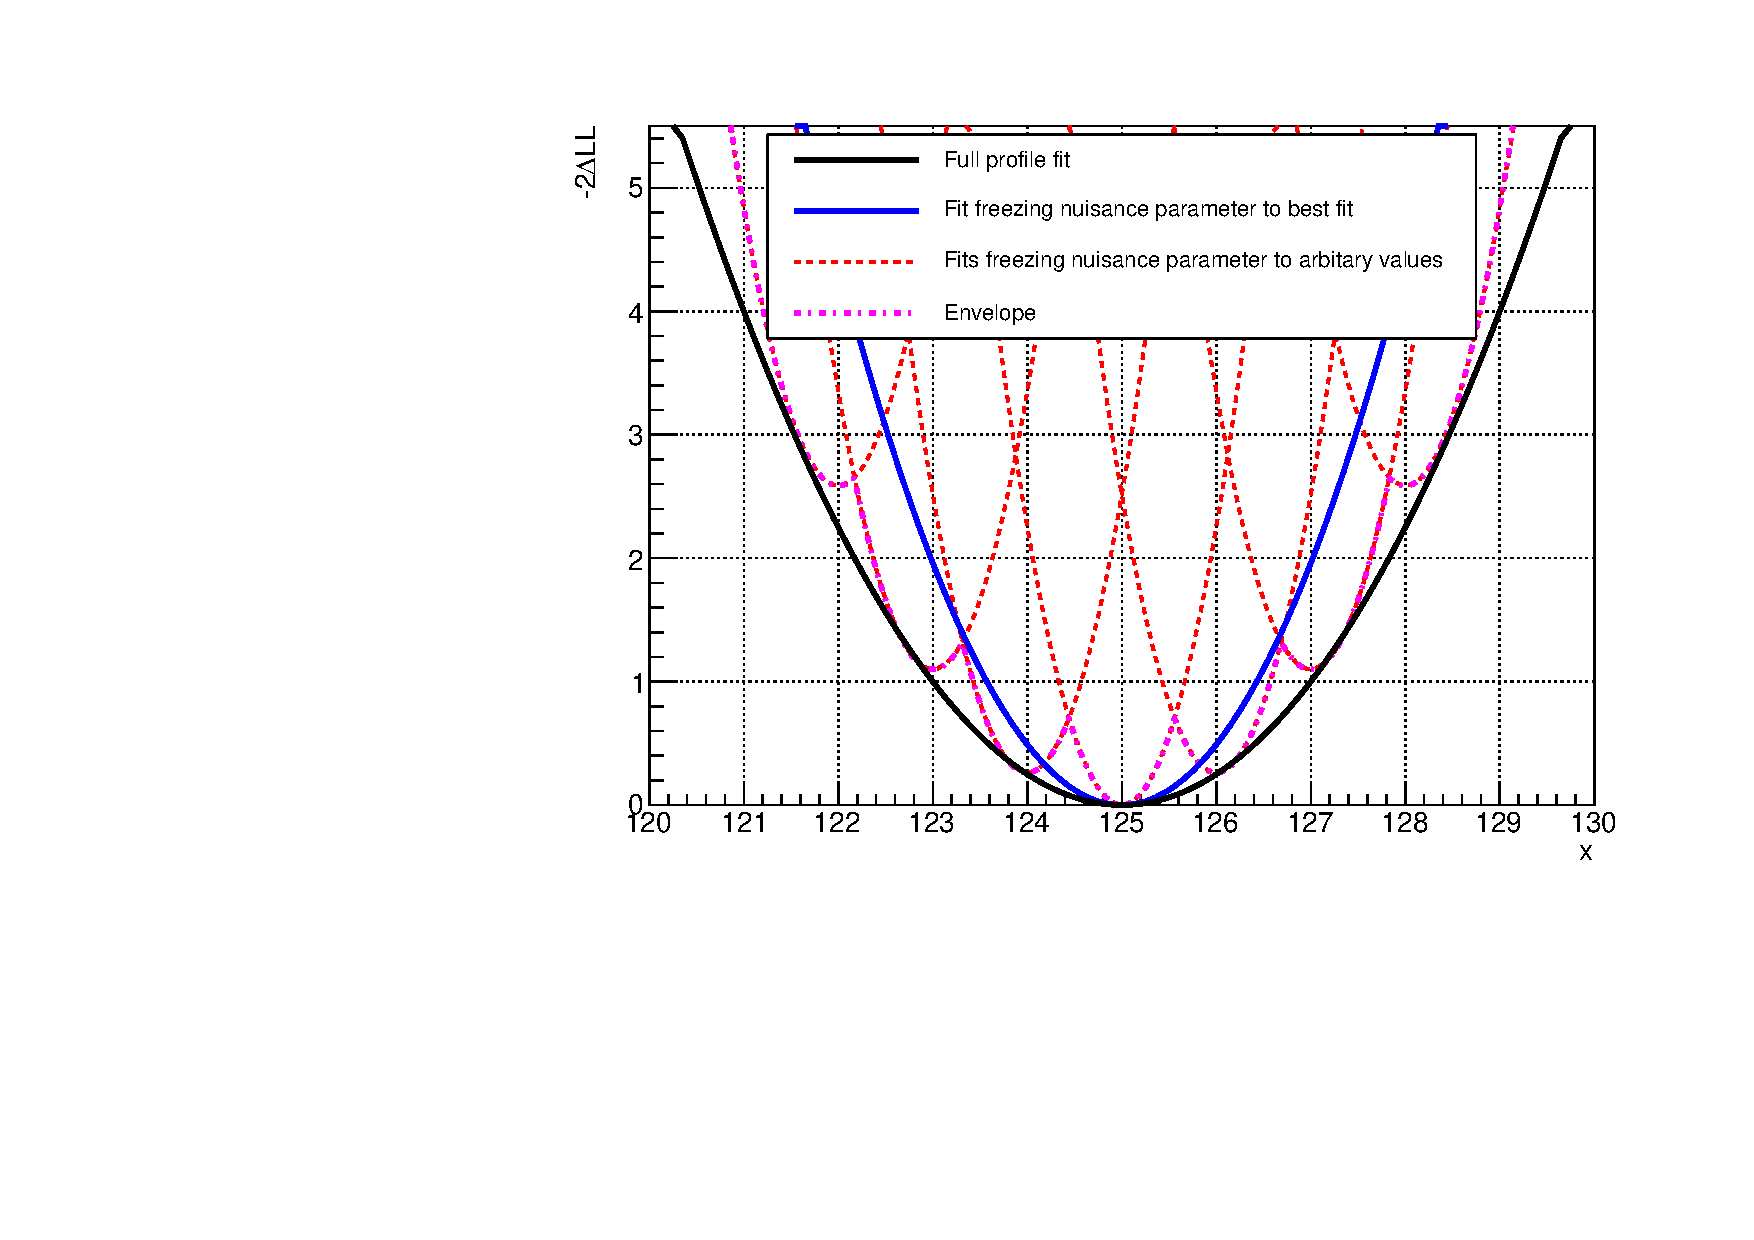
\includegraphics[width=0.8\textwidth]{analysis/plots/envelope_explain.pdf}
  \caption[Conceptual idea of the method of likelihood profiling]{Conceptual idea of the method of ``profiling the likelihood". Here the \NLL is scanned as a function of a physical parameter of interest $x$ with a nuisance parameter $\theta$ in three cases: 1) where $\theta$ is freely floating (black line), 2) where $\theta$ is set to its value at the \NLL minimum (blue line), 3) for several arbitary choices of $\theta$ (red line). The green line shows the ``envelope" around the total minimum over several discrete choices of $\theta$. After an infitinte sampling of $\theta$ the green line would match the black.}
  \label{fig:envelope_explain1}
\end{center}
\end{figure}

In this analysis the background parametrisation is entirely unknown. So in principle if we could sample the infinite phase space of possible function choices we could use the method just described to profile the choice. In this way we find the function that minimises the negative likelihood for any given value of the parameter of interest $x$. This will then pick the function which fits the data best (minimises the neagtive likelihood) but can enlarge the error given that many different functions are tried.
Lets now consider a simplified case of the real situation. Imagine we have a large steeply falling background which can be parametrised by two possible choices: a single term power law, $x^{-p}$, and a single term exponential, $e^{-px}$. We have a small Gaussian-like signal component and our \POI is the size of this signal, $\mu$. The best fit distributions are shown for a generated pseudo-dataset in the left hand plot of Fig.~\ref{fig:envelope_explain2}. The right hand plot of Fig.~\ref{fig:envelope_explain2} shows the likelihood scan across the parameter $\mu$, which represents the size of the signal, for the two chosen functions (blue and red lines). The envelope (the minimum of the negative likelihood across both function choices) is shown as the yellow dashed line. One can see that the global best fit from the envelope is at a value of $\mu=2.83$ which is that obtained with the power law function. The $1\sigma$ error (the point where the \NLL crosses 1) is unchanged in the envelope with respect to the result using the power law function alone. However, the $2\sigma$ error (the point where the \NLL crosses 4) is increased with respect to the result using the power law function alone. This is the principal behind the ``envelope" background method. One can see that it is analagous to using a normal nuisance parameter which can only take discrete values. In this case the discrete values index which function is chosen. It means that a specific function choice never has to be made and the error on a given value will increase to account for situations where two or more functions give a similarly good fit. However, there is one more important feature of the method which must be discussed before it can be applied to the data.

\begin{figure}
  \begin{center}
    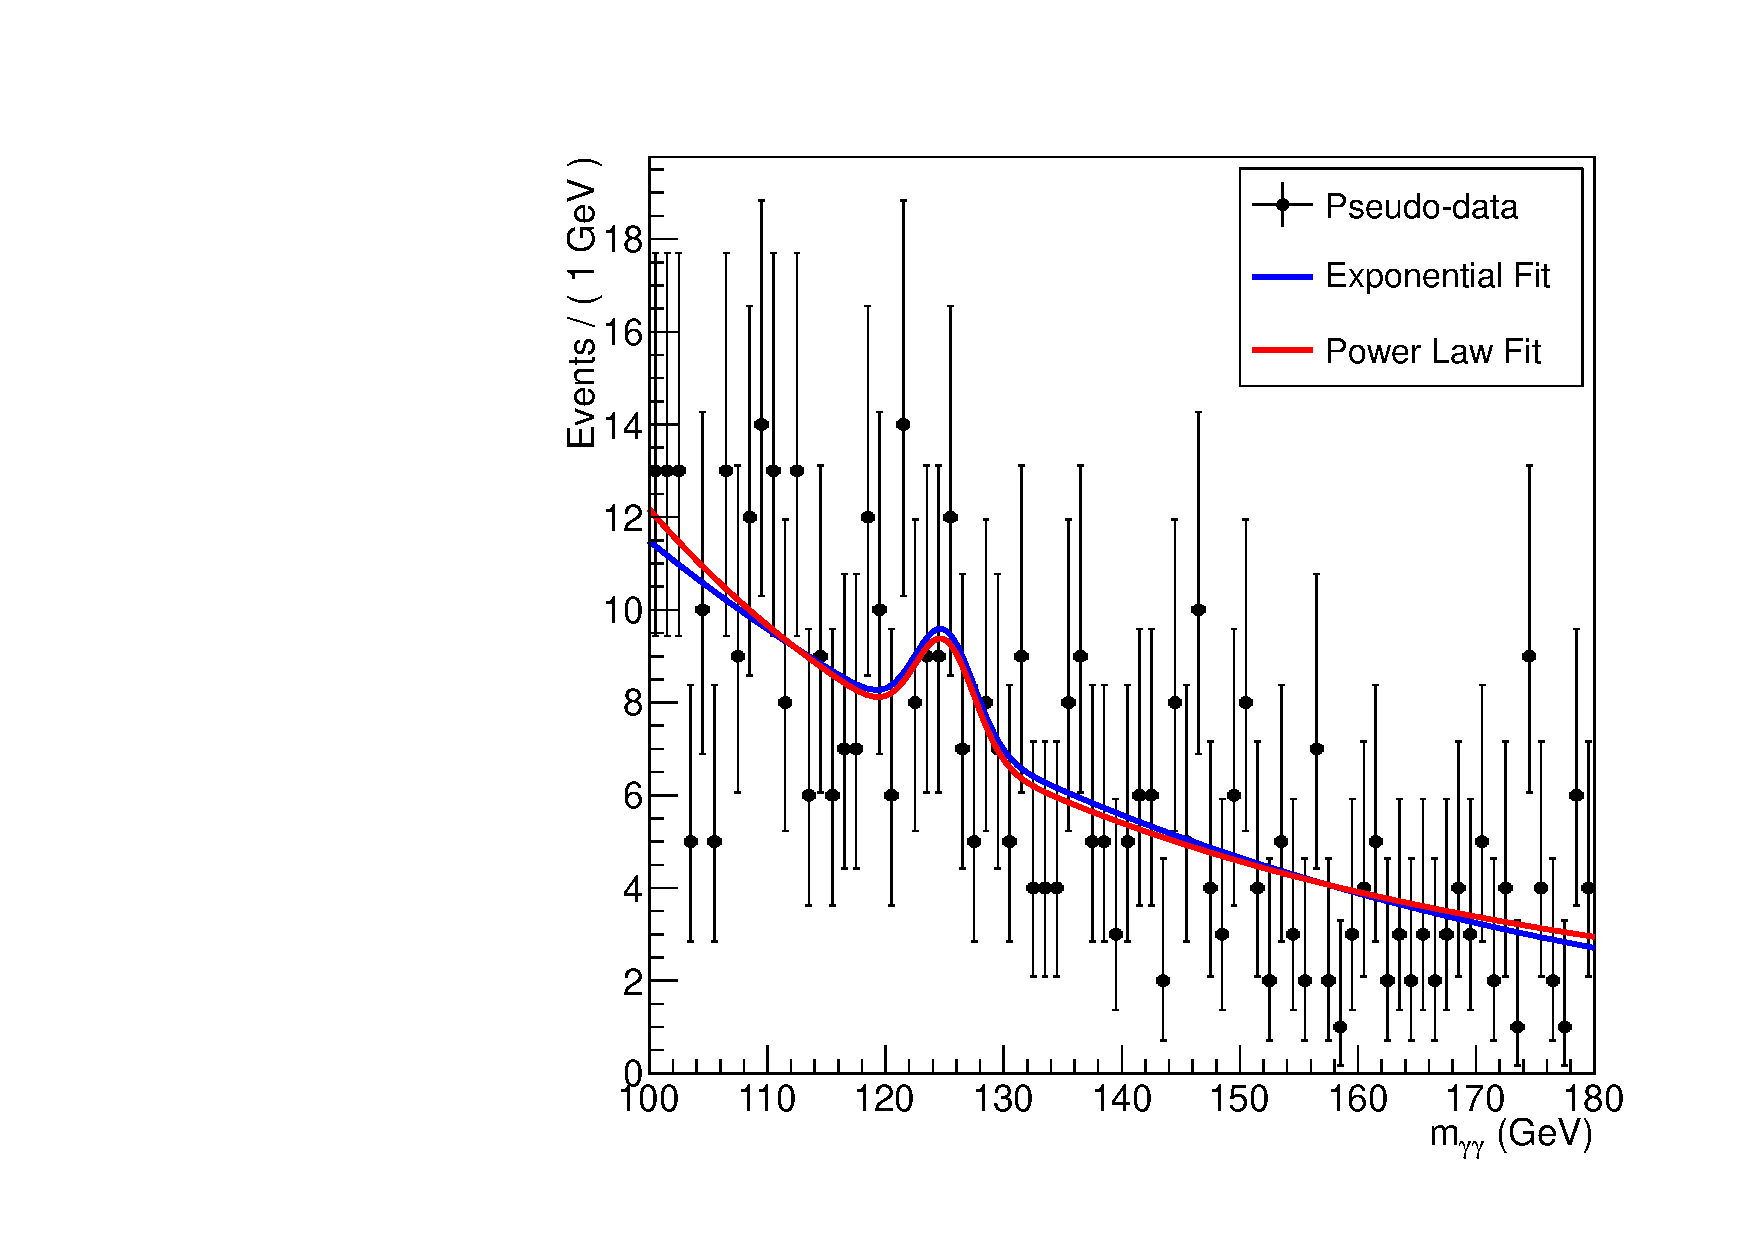
\includegraphics[width=0.49\textwidth]{analysis/plots/envelope_explain2.pdf}
    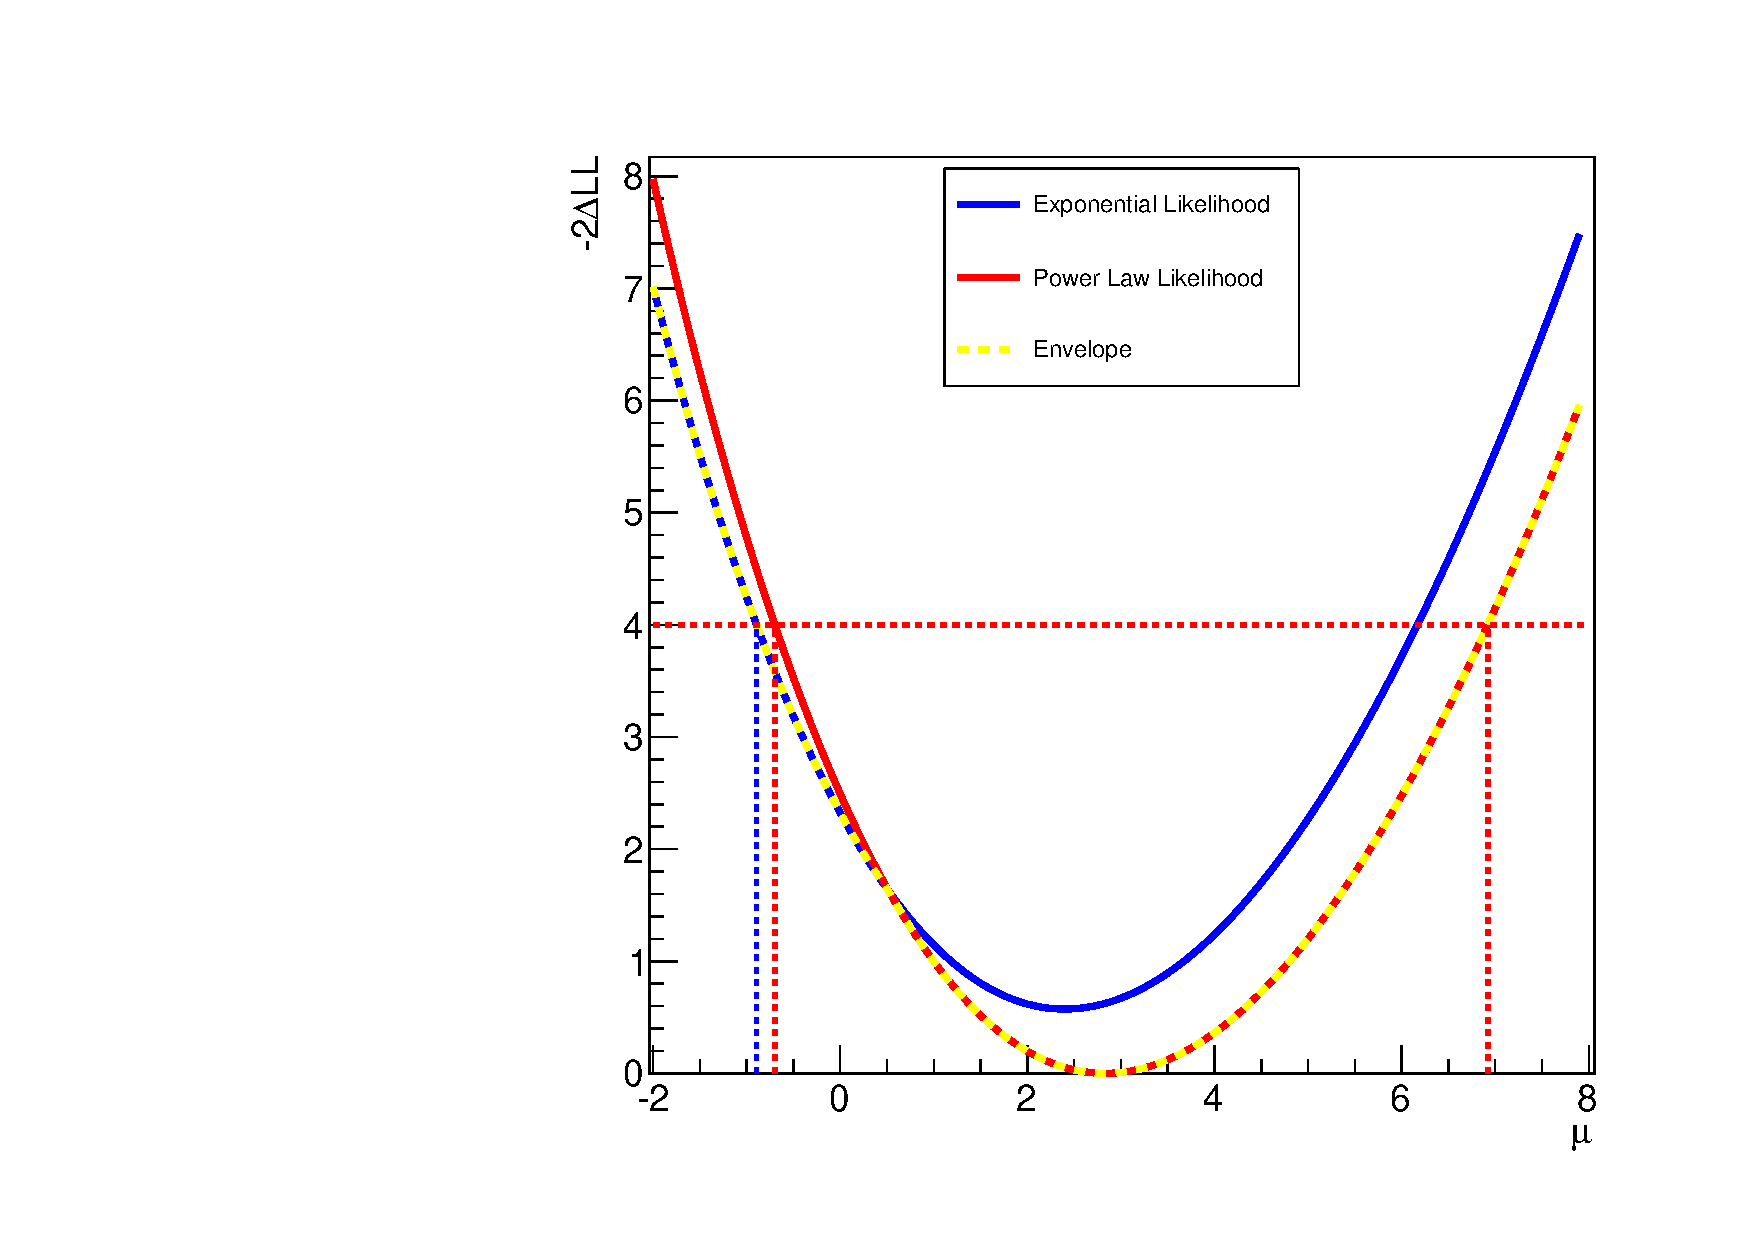
\includegraphics[width=0.49\textwidth]{analysis/plots/envelope_explain3.pdf}
    \caption[A toy example of using the envelope method for estimating the background]{An example of using the envelope in a realistic situation. The plot on the left shows a signal plus background fit to some pseudo-data using two different background function choices; a single term power law (red) and a single term exponential (blue). The plot on the right shows the profile likelihood curve for the signal size, $\mu$, for the two different function choices. The global minimum is at $\mu=2.83$ and the power law is used as the background choice. The envelope likelihood curve, profiling over the function choices is shown as the yellow dashed line.}
    \label{fig:envelope_explain2}
  \end{center}
\end{figure}

The concept of the ``envelope" method has now been demonstrated with a simplified example in which two function choices were profiled and both these functions had one free parameter. However we would like to be able to sample as much of the function phase space possible (i.e.~as many functions as we can) which means there will be choices with different numbers of free parameters. Two functions of the same type but of a different order may give a very similar looking fit but functions with more free parameters are more flexible and thus will give a lower negative likelihood value. For example consider the functions $E_{1} = e^{-p_{1}x}$ and $E_{2} = f_{1}e^{-p_{1}x}+(1-f_{1})e^{-p_{2}x}$, which are first and second order exponential sums and have one and three free parameters respectively, not including an overall normalisation term. There may be a case where these give an identical fit (as $f_{1}\to 1$ or $p_{1}\to p_{2}$) however the negative log likelihood will always be lower for a higher parameter fit and therefore the higher order function would always be the minimum of the envelope. This means that for any embedded class of functions, the function which gives the global minimum of the likelihood will be of the highest order allowed. Consequently, a correction scheme has been devised to avoid this problem and to penalise functions in the envelope which have more free parameters but don't necessarily fit the data any better.

The negative log likelihood gets redefined as,
\begin{equation}
  -2\mathrm{LL} = -2\ln(\mathcal{L}) + cN_{p},
\end{equation}
where $\mathcal{L}$ is the likelihood for the function, $N_{p}$ is the number of free parameters in that function and $c$ is a constant correction term. Two correction schemes were studied, for values of $c=1$ and $c=2$. The motivation for choosing $c=2$ is an application of the Akaike information criterion, described in Ref.~\cite{akaike}, which states that for large sample sizes the corrected likelihood is,
\begin{equation}
  A = -2\ln(\mathcal{L}) + 2N_{p}.
\end{equation}
It can be seen that the correction term here is $2N_{p}$, which gives a value of $c=2$, in others words a correction of 2 per free parameter. 

The argument for using a correction of $c=1$ is a little more natural and arises from the assumption that in the high statistics limit for a binned dataset, $\NLL\approx\chi^{2}$. Given a value of the $\chi^{2}$ one can calculate the $\chi^{2}$ $p$-value given the number of degrees of freedom, $N$, which is equal to the number of bins, $b$, minus the number of free parameters in the fit function, $N_{p}$. Thus the $p$-value can be expressed as $p(\chi^{2},b-N_{p})$. One can then determine a new chi-squared value, $\chi^{\prime 2}$, defined as the one which would give the equivalent $p$-value but with a different number of degrees of freedom, namely the one in which there are no free parameters in the fit, $p(\chi^{\prime 2},b)$ . It can be seen that there is now an expression for $\chi^{\prime 2}$, which is approximately equivalent to a new \NLL (now relative to the best possible fit, given the data), which is independet of the number of fit parameters, $N_{p}$, and thus the corrected likelihood is given by,
\begin{equation}
  -2\mathrm{LL} = -2\ln(\mathcal{L}) + \chi^{\prime 2} - \chi^{2}.
\end{equation}
The correction term, $\chi^{\prime 2} -\chi^{2}$, depends on the number of bins, the number of free fit parameters and the quality of the original fit (the $\chi^{2}$ $p$-value). Figure~\ref{fig:envelope_chi2_correction} shows how the size of the correction varies for functions with different numbers of fit parameters. It can be seen that on average the correction is given by,
\begin{equation}
  \chi^{\prime 2} - \chi^{2} \approx N_{p}.
\end{equation}
\begin{figure}
  \begin{center}
    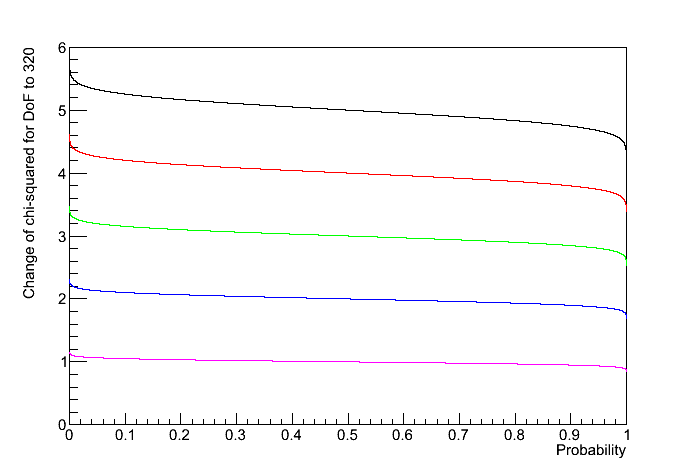
\includegraphics[width=0.49\textwidth]{analysis/plots/ChisqConv1.png}
    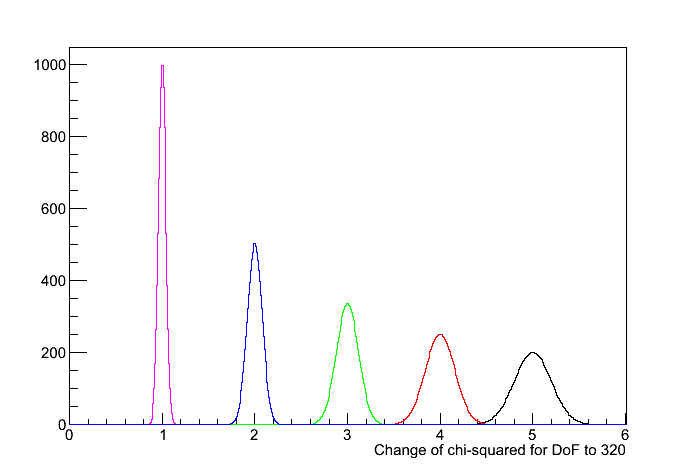
\includegraphics[width=0.49\textwidth]{analysis/plots/ChisqConv2.png}
    \caption[An estimation of the correction required in the envelope method]{The value of the correction, $\chi^{\prime 2} - \chi^{2}$, as a function of the fit $p$-value for a fit with 320 bins is shown on the left. The projection of the correction integrated uniformaly over $p$-values is shown on the right. The five different coloured lines represented fit functions with different numbers of free parameters, ranging from one free parameter (pink) up to five free parameters (black).}
    \label{fig:envelope_chi2_correction}
  \end{center}
\end{figure}
The correction scheme used in the analysis was chosen to be $c=1$. This was decided using empirical results of studying the impact on the bias and error coverage when fitting the physical parameters of the signal yield, $\mu$, and the signal position, \mH, using the envelope method with either correction scheme. Before we cover the results and conclusions of this study, let's first discuss how one decides which functions to include in the envelope.

In principal it would be beneficial to choose any and every function one can think of that can reasonably describe a falling spectrum. In practise this is unfeasible as the combinatorics of the problem rapidly spiral out of control. If an analysis has multiple categories, $N_{c}$, and one chooses multiple background functions in each category, $N_{f}$, then the number of combinations goes like $N_{f}^{N_{c}}$ which rapidly makes the problem computationally impossible. Instead, one has to choose a smaller number of functions which reasonably cover the phase space of infinite functions. The functions used in this analysis come in four main classes. They are as follows (note an overall normalisation term is not included in the equations below),

\begin{itemize}
  \item \textit{Exponential recursive sum} - a sum of terms like $e^{-px}$.
    \begin{equation}
      p(x) = c_{1}e^{-p_{1}x} + (1-c_{1})c_{2}e^{-p_{2}x} + (1-c_{2})c_{3}e^{-p_{3}x} + ... + (1-c_{n-1})e^{-p_{n}x}
    \end{equation}
    \begin{itemize}
      \item This has $2n-1$ free parameters per order. The functions are labelled by the number of free parameters so the lowest order is \texttt{exp1} then \texttt{exp3}, \texttt{exp5} and so on.
    \end{itemize}

  \item \textit{Power law recursive sum} - a sum of terms like $x^{-p}$.
    \begin{equation}
      p(x) = c_{1}x^{-p_{1}} + (1-c_{1})c_{2}x^{-p_{2}} + (1-c_{2})c_{3}x^{-p_{3}} + ... + (1-c_{n-1})x^{-p_{n}}
    \end{equation}
    \begin{itemize}
      \item This has $2n-1$ free parameters per order. The functions are labelled by the number of free parameters so the lowest order is \texttt{pow1} then \texttt{pow3}, \texttt{pow5} and so on.
    \end{itemize}

  \item \textit{Laurent series} - The best fit value for a single order power term is around -4.3. Consequently we use a Laurent-like series of a sum of terms like $x^{-n}$ expanded around $x^{-4}$.
    \begin{equation}
      p(x) = c_{1}x^{-4} + (1-c_{1})c_{2}x^{-5} + (1-c_{2})c_{3}x^{-3} + (1-c_{3})c_{4}x^{-6} + ...
    \end{equation}
    \begin{itemize}
      \item This has $n-1$ free parameters per order. The functions are labelled by the number of free parameters so the lowest order is \texttt{lau1} then \texttt{lau2}, \texttt{lau3} and so on.
    \end{itemize}

  \item \textit{Bernstein polynomials} - These are polynomials in the Bernstein basis~\cite{bernsteins1,bernsteins2}. A Bernstein polynomial of degree $n$ is given by,
  \begin{equation}
    p(x) = \displaystyle\sum_{1}^{n}c_{i}\frac{n!}{i!(n-i)!}x^{i}(1-x)^{n-i}
    \label{eq:bernsteins}
  \end{equation}
  \begin{itemize}
    \item This has $n$ free parameters per order. The functions are labelled by the number of free parameters so the lowest order is \texttt{pol1} then \texttt{pol2}, \texttt{pol3} and so on.
  \end{itemize}
\end{itemize}

One then has to determine which order functions of each of these classes is used in the envelope for a given dataset. To pick the lowest order included in the envelope a simple goodness of fit test is used and has the loose requirement that the $\chi^{2}$ $p$-value of the fit is greater than 0.01. To pick the higest order used in the envelope an $f$-test style requirement is imposed~\cite{ftest}. If two functions of the same class have $n$ and $n+m$ free parameters respectively then, in the high statistics limit, the difference in \NLL between the two functions is distributed as $\chi^{2}$ with $m$ degrees of freedom. Consequently the difference in \NLL between the two fits is converted into a $\chi^{2}$ $p$-value and the next higher order function is included if $p<0.1$. In other words if the higher order function does not improve the fit it is not included. This determines which functions are included in the envelope for each category and ranges anywhere between 4 and 9. It should be noted that the requirements to include a function are intentionally loose so that as much of the ``function-space" is sampled as possible.

In order to assess the bias and coverage properties of the envelope method a few functions are chosen as ``truth" models from which to generate pseudo-data and test the statistical validity of the method. A single function of each class is chosen as a ``truth" model and the order determined by the same $f$-test but with a tighter requirement that $p<0.05$. These models are first fit to the data and then the pseudo-data generated from these values. The comparison of the systematic bias to statistical uncertainty is determined by the pull distribution,
\begin{equation}
  pull(\mu) = \frac{\mu_{fit} - \mu_{inj}}{\sigma_{fit}},
\end{equation}
where $\mu_{inj}$ is the injected signal strength in the toy, $\mu_{fit}$ is the fitted signal strength per toy and $\sigma_{fit}$ is the error on the fitted signal strength per toy. The systematic bias to statistical comparison is then the deviation of the mean of the distribution from zero as compared to the width of this distribution. An unbiased method will give a mean close to 0 and a method which covers accurately will give a width equal to 1. The $X\sigma$ coverage is defined as the fraction of toys for which $\mu_{fit}-X\sigma_{fit}\leq\mu_{inj}\leq\mu_{fit}+X\sigma_{fit}$.

When using a correction factor of $c=1$, the systematic bias on the signal strength is less than 14\% of the statistical error from the fit and the coverage is accurate for 0.5, 1, 2 and 3$\sigma$ (all the points tested). This was found to be true when generating toy experiments for a range of different signal strengths and for signal at different mass values. The bias and coverage have also been tested when removing the ``truth" model from the set of envelope functions, when removing all functions of the same class as the ``truth" model and when using various convoluted truth models such as a histogram spline of the data~\cite{regression_spline}, a kernel density estimator (sum of Gaussians)~\cite{kde} and a hybrid of different functions patched together. All of these cases also demonstrated a reasonable level of bias and coverage. 

When using a correction factor of $c=2$ the systematic bias is larger than this, in extreme cases it can reach 30\% of the statistical uncertainty and in these cases it is common that the method undercovers especially at higher standard deviations, $\sigma$. Consequently, for this analysis a correction factor of $c=1$ is chosen. The tests described above to ascertain the statistical validity of the method are performed for each individual category of the analysis and furthermore for the categories combined together in years and the whole ensemble of categories. The method has sensible behaviour in all of these cases.

The invariant mass distributions with the different envelope functions, after having been fit to the data, for each of the analysis categories are shown in Figs.~\ref{fig:multipdf1}-\ref{fig:multipdf6}.

\begin{figure}
  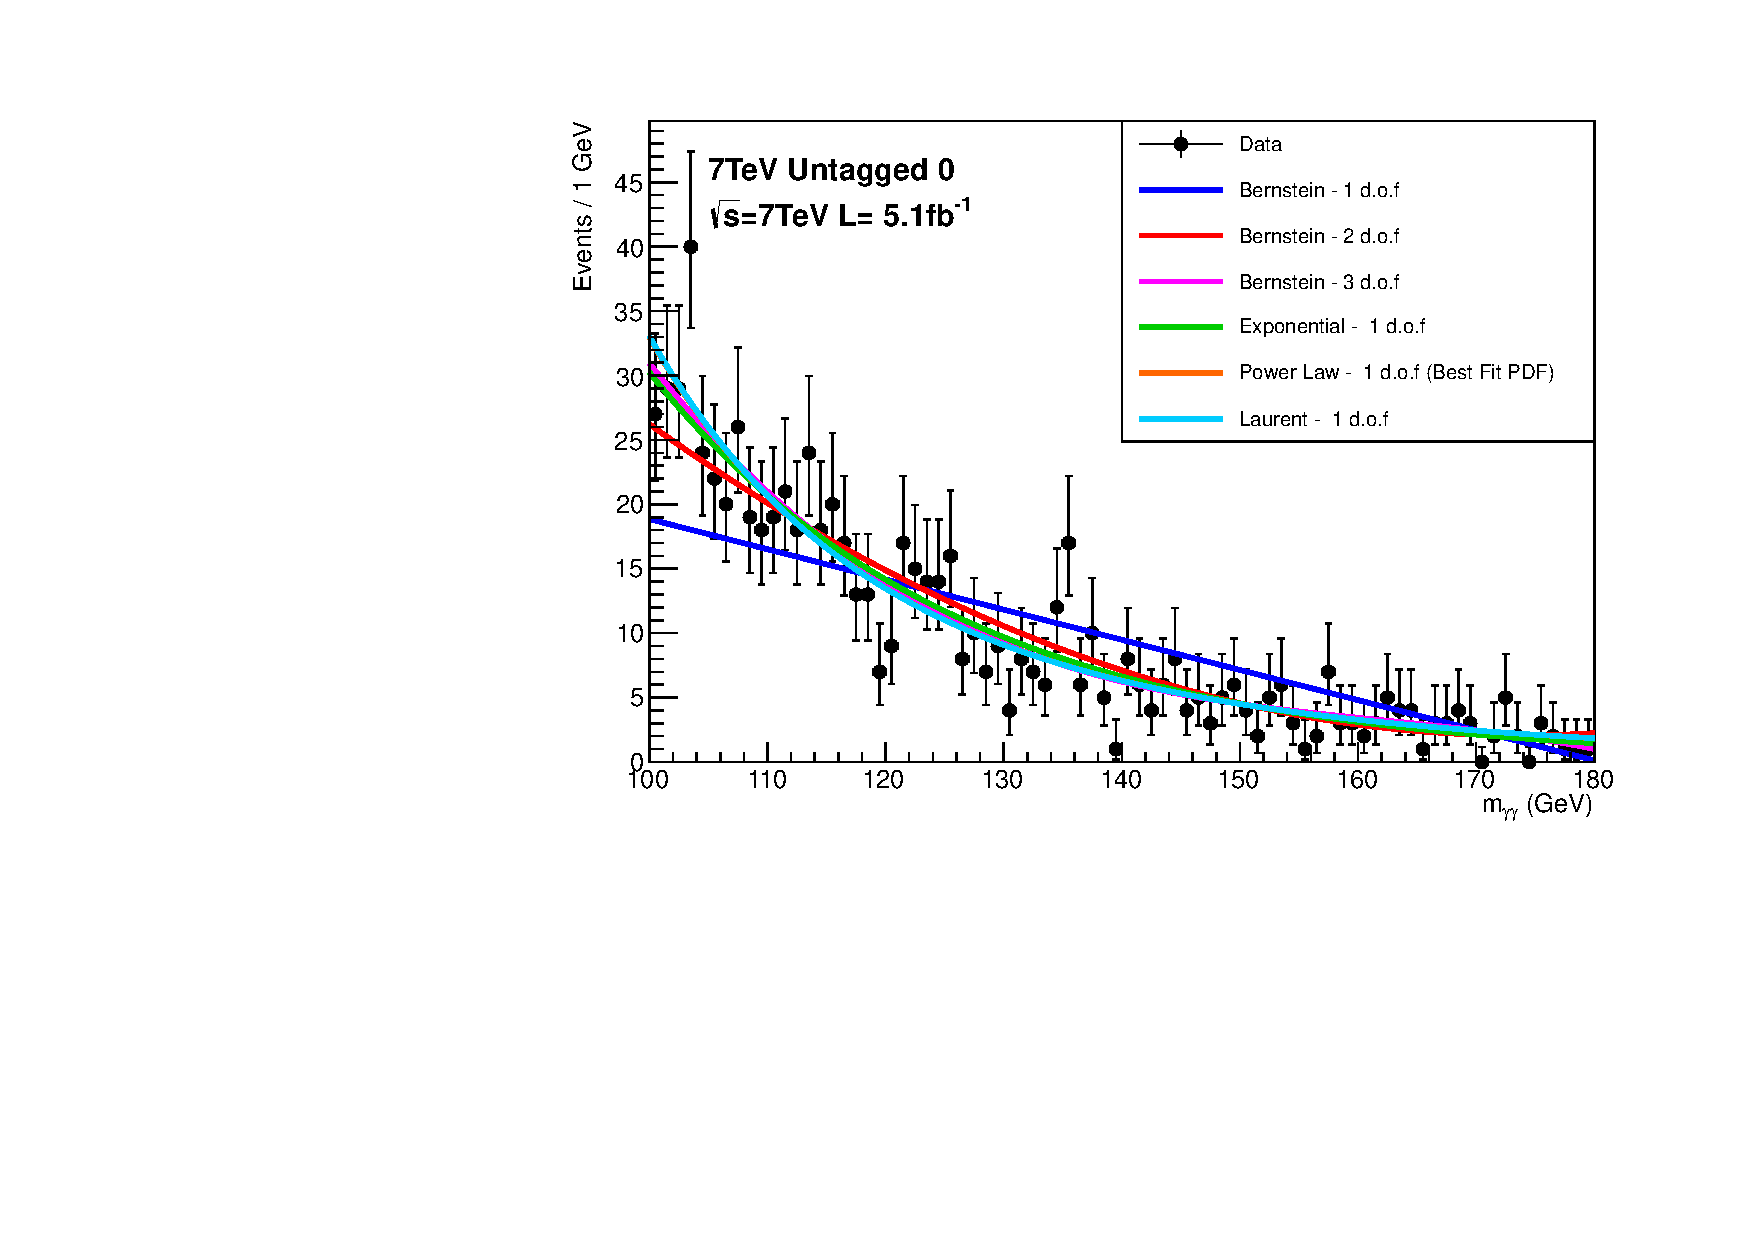
\includegraphics[width=0.49\textwidth]{analysis/plots/multipdf_plots/cat0_7TeV.pdf}
  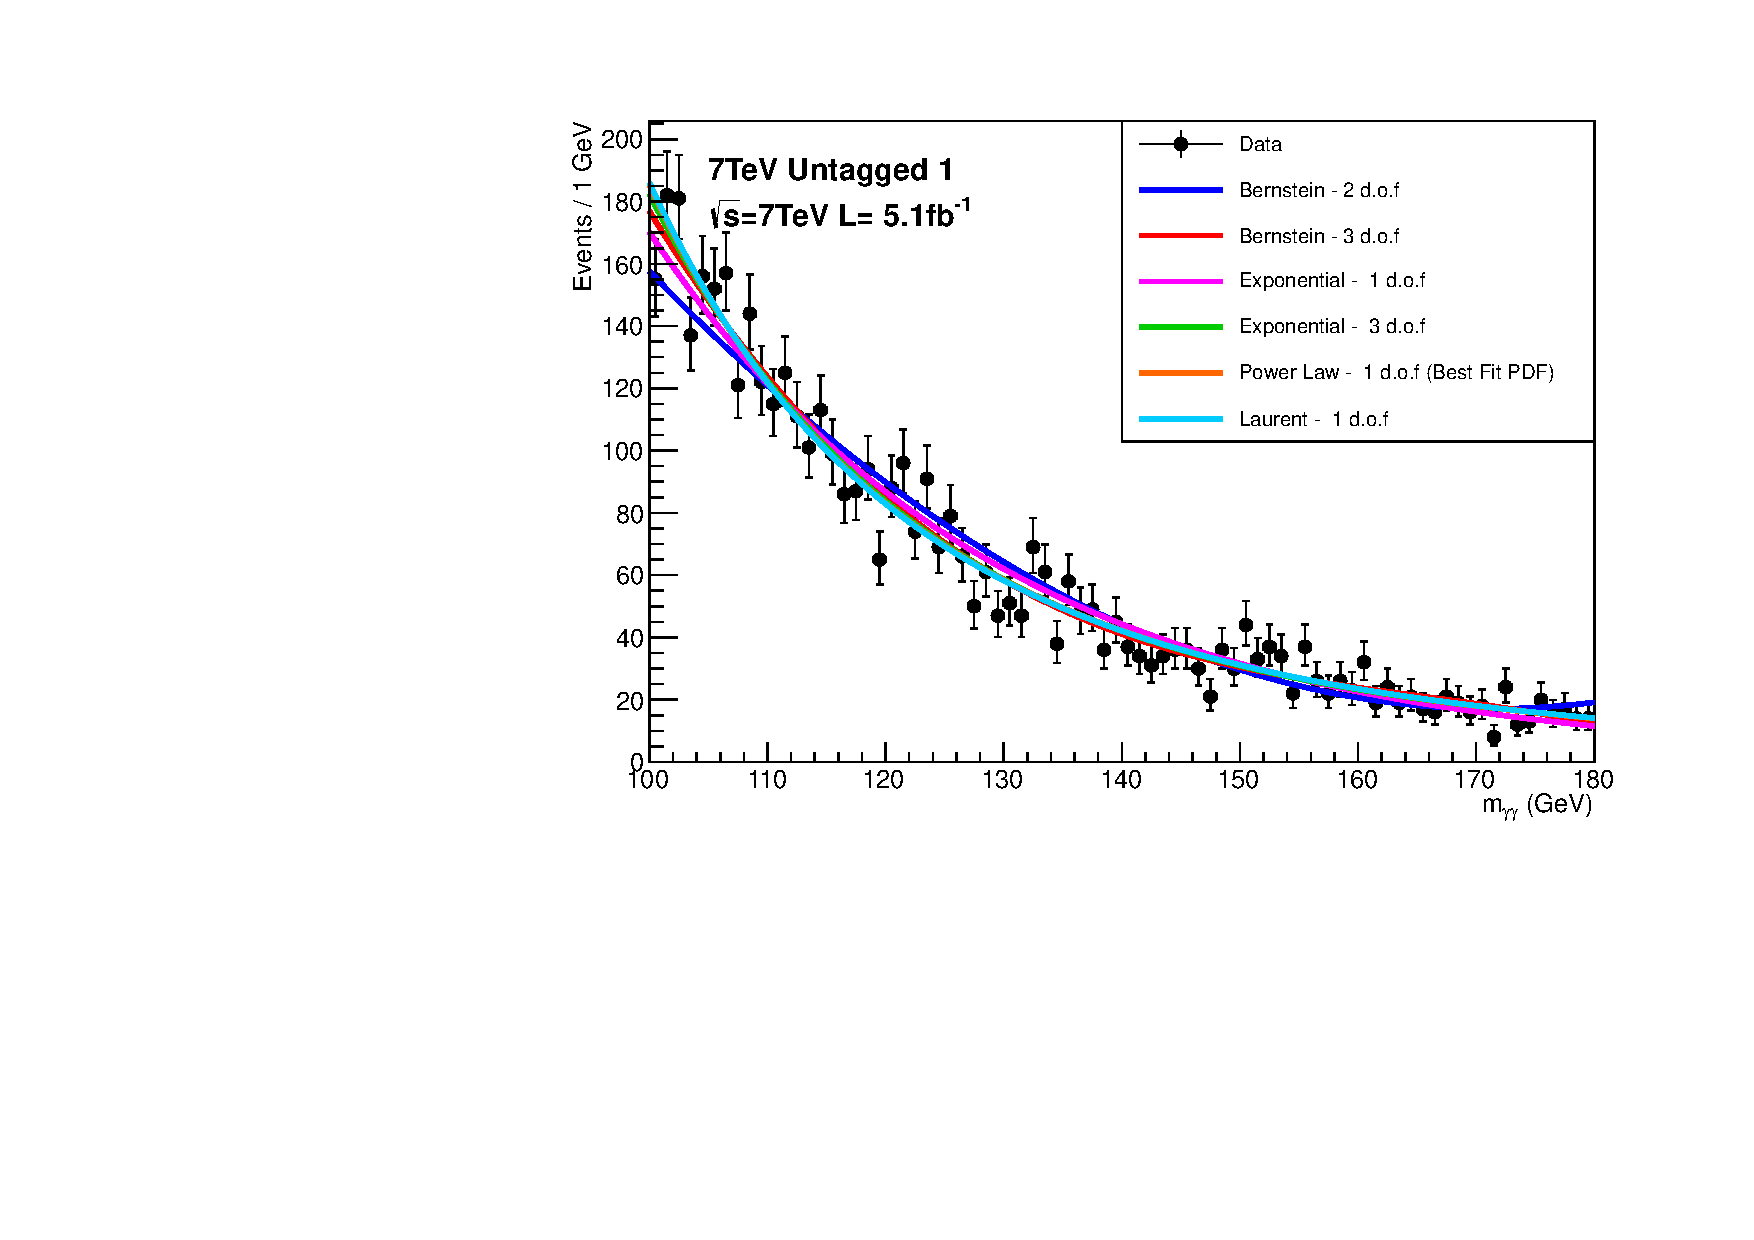
\includegraphics[width=0.49\textwidth]{analysis/plots/multipdf_plots/cat1_7TeV.pdf}\\
  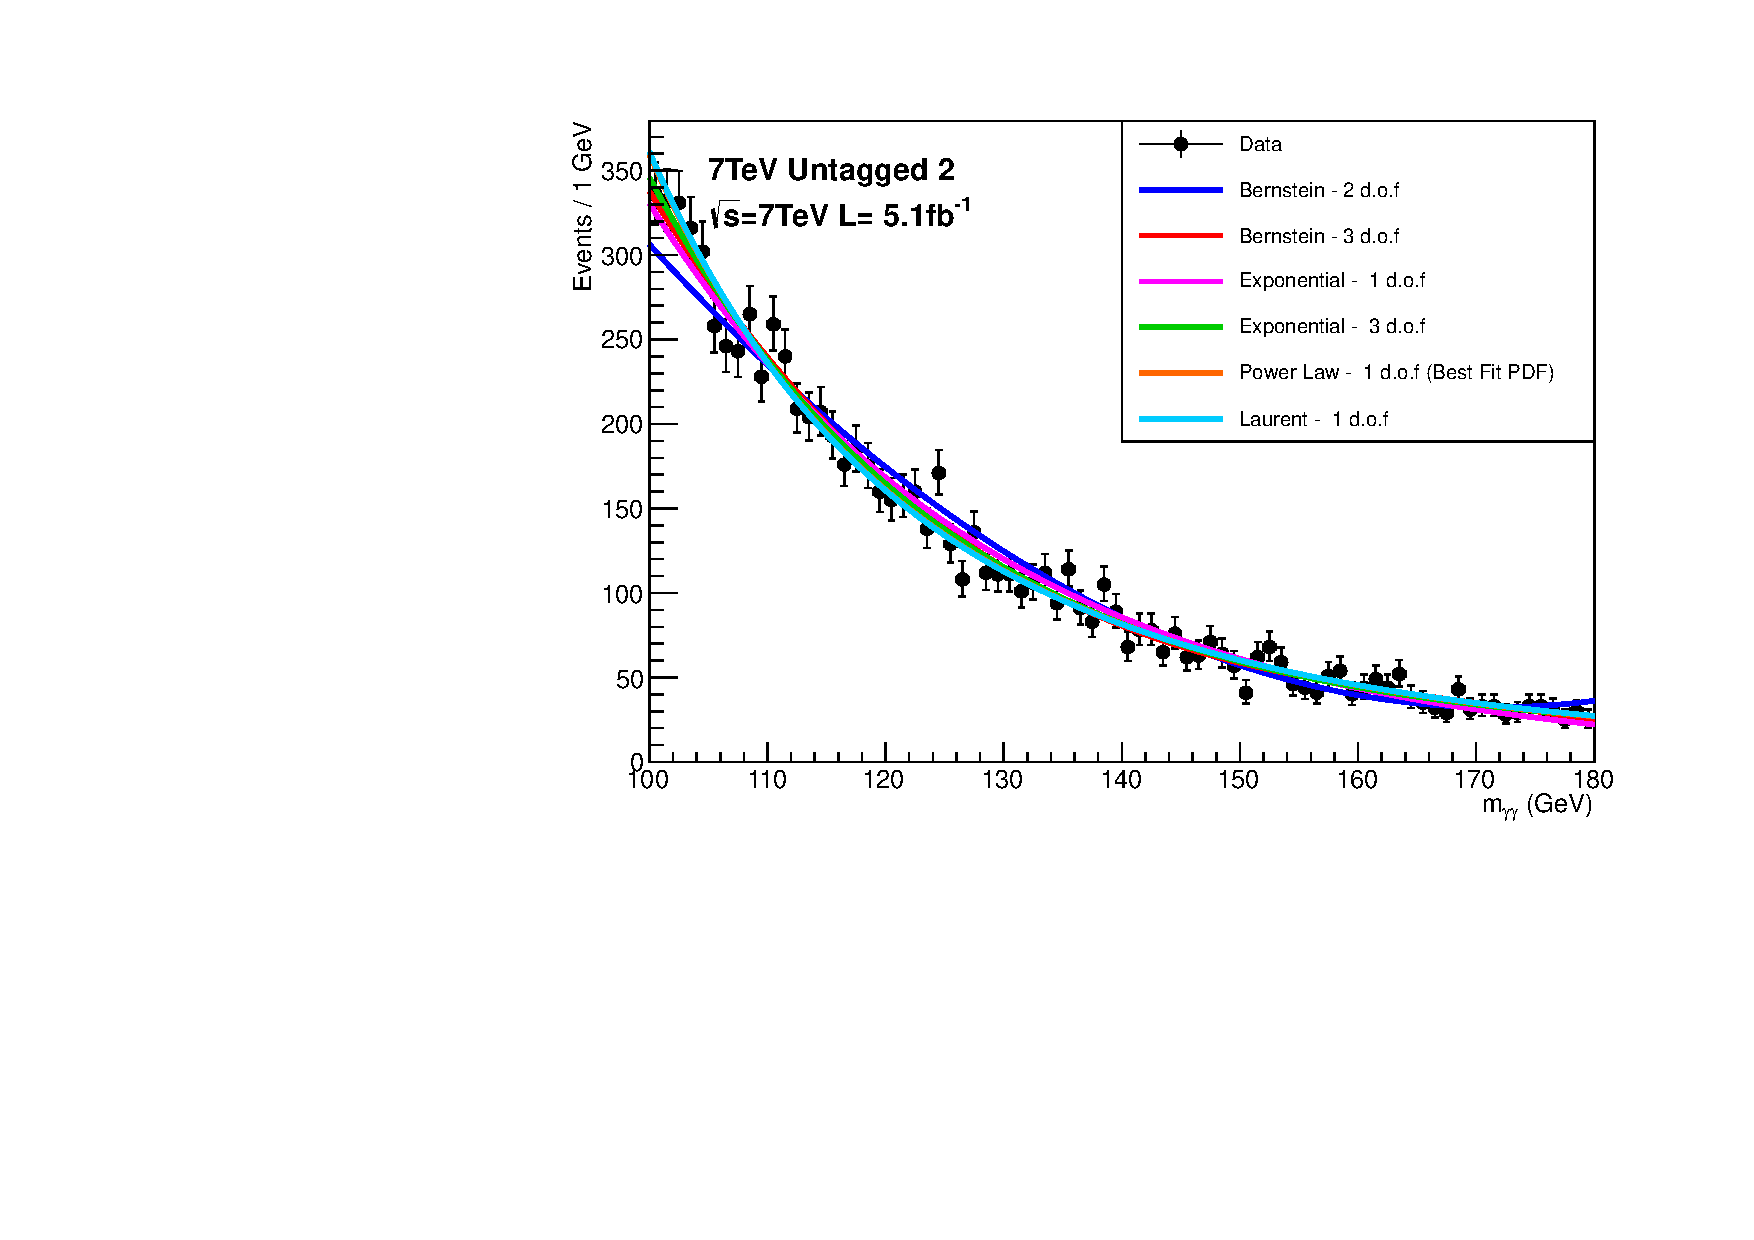
\includegraphics[width=0.49\textwidth]{analysis/plots/multipdf_plots/cat2_7TeV.pdf}
  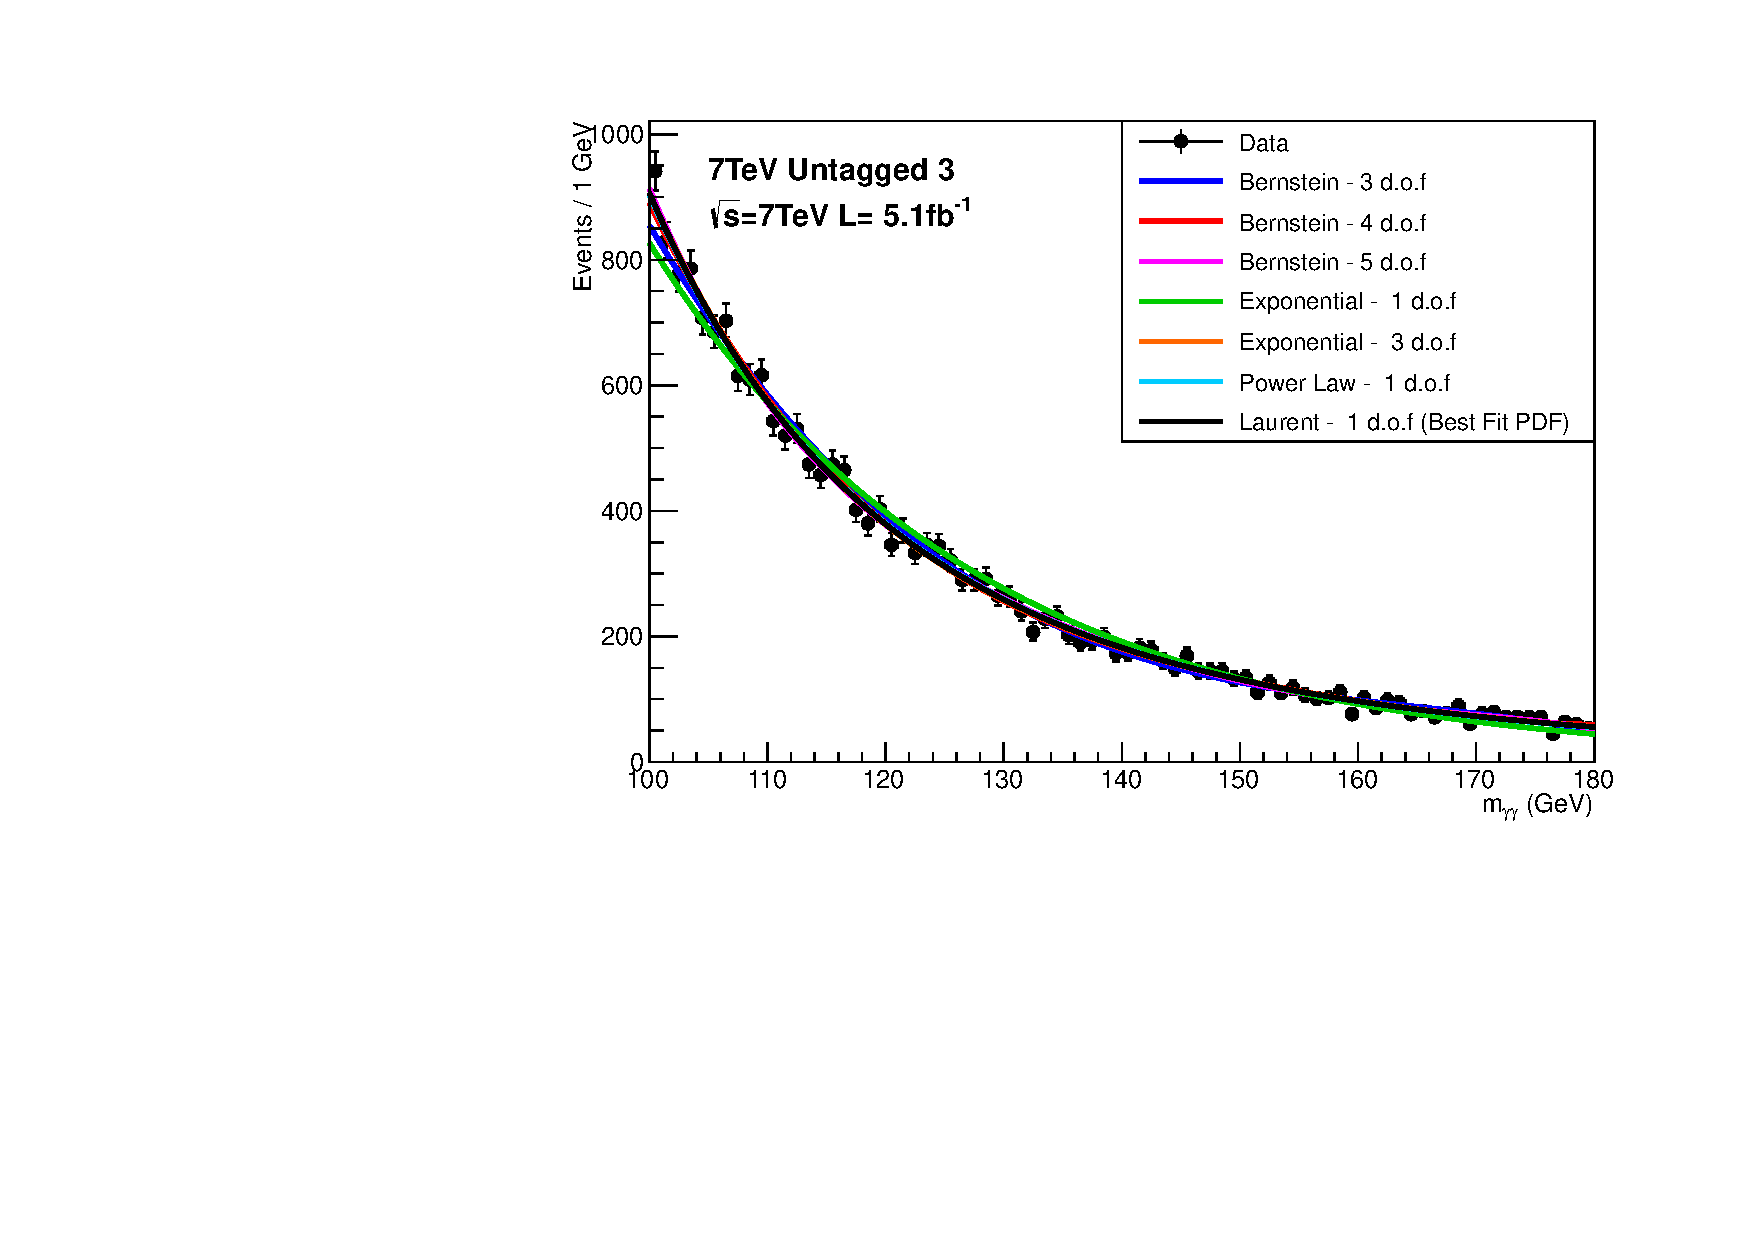
\includegraphics[width=0.49\textwidth]{analysis/plots/multipdf_plots/cat3_7TeV.pdf}\\
  \caption{The diphoton invariant mass distribution and the function choices for the background envelope for the inclusive categories in the 7~\TeV dataset.}
  \label{fig:multipdf1}
\end{figure}

\begin{figure}
  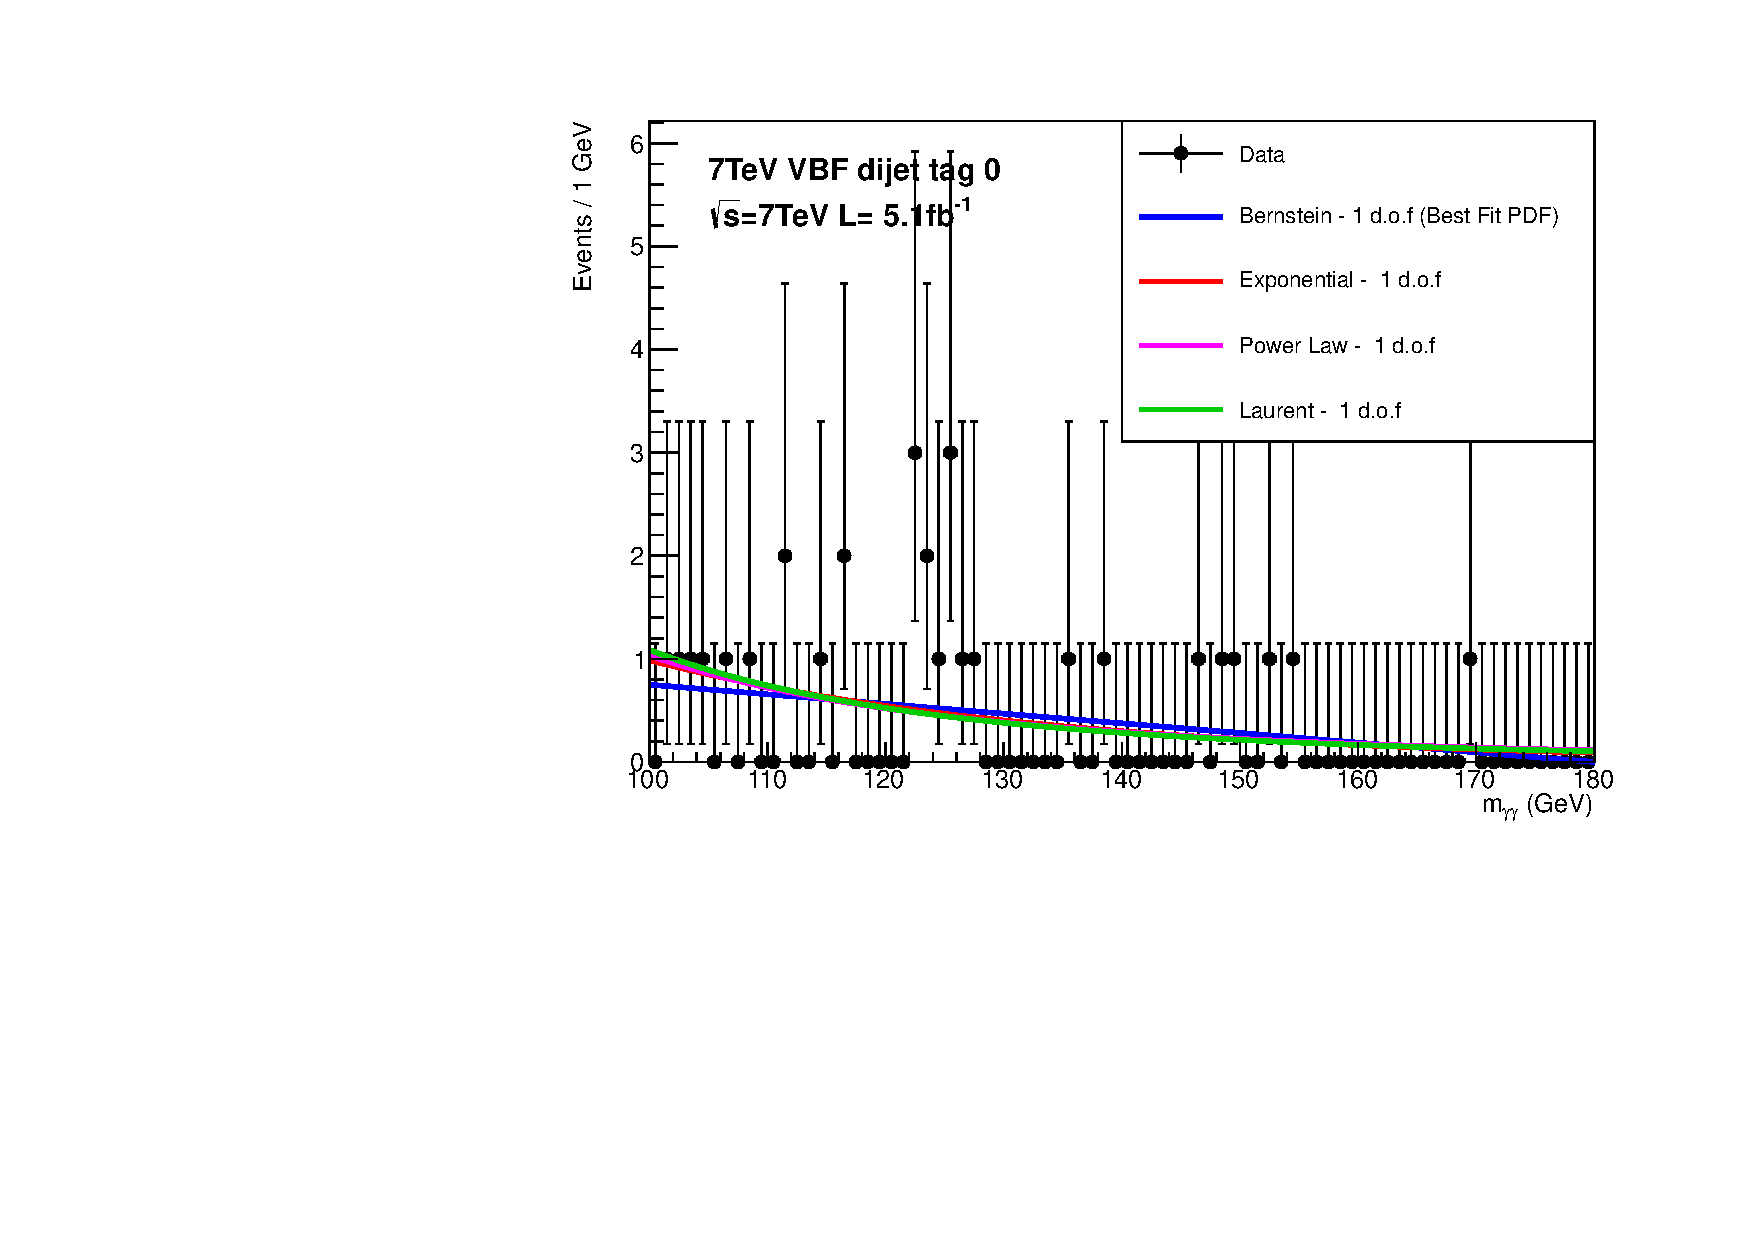
\includegraphics[width=0.49\textwidth]{analysis/plots/multipdf_plots/cat4_7TeV.pdf}
  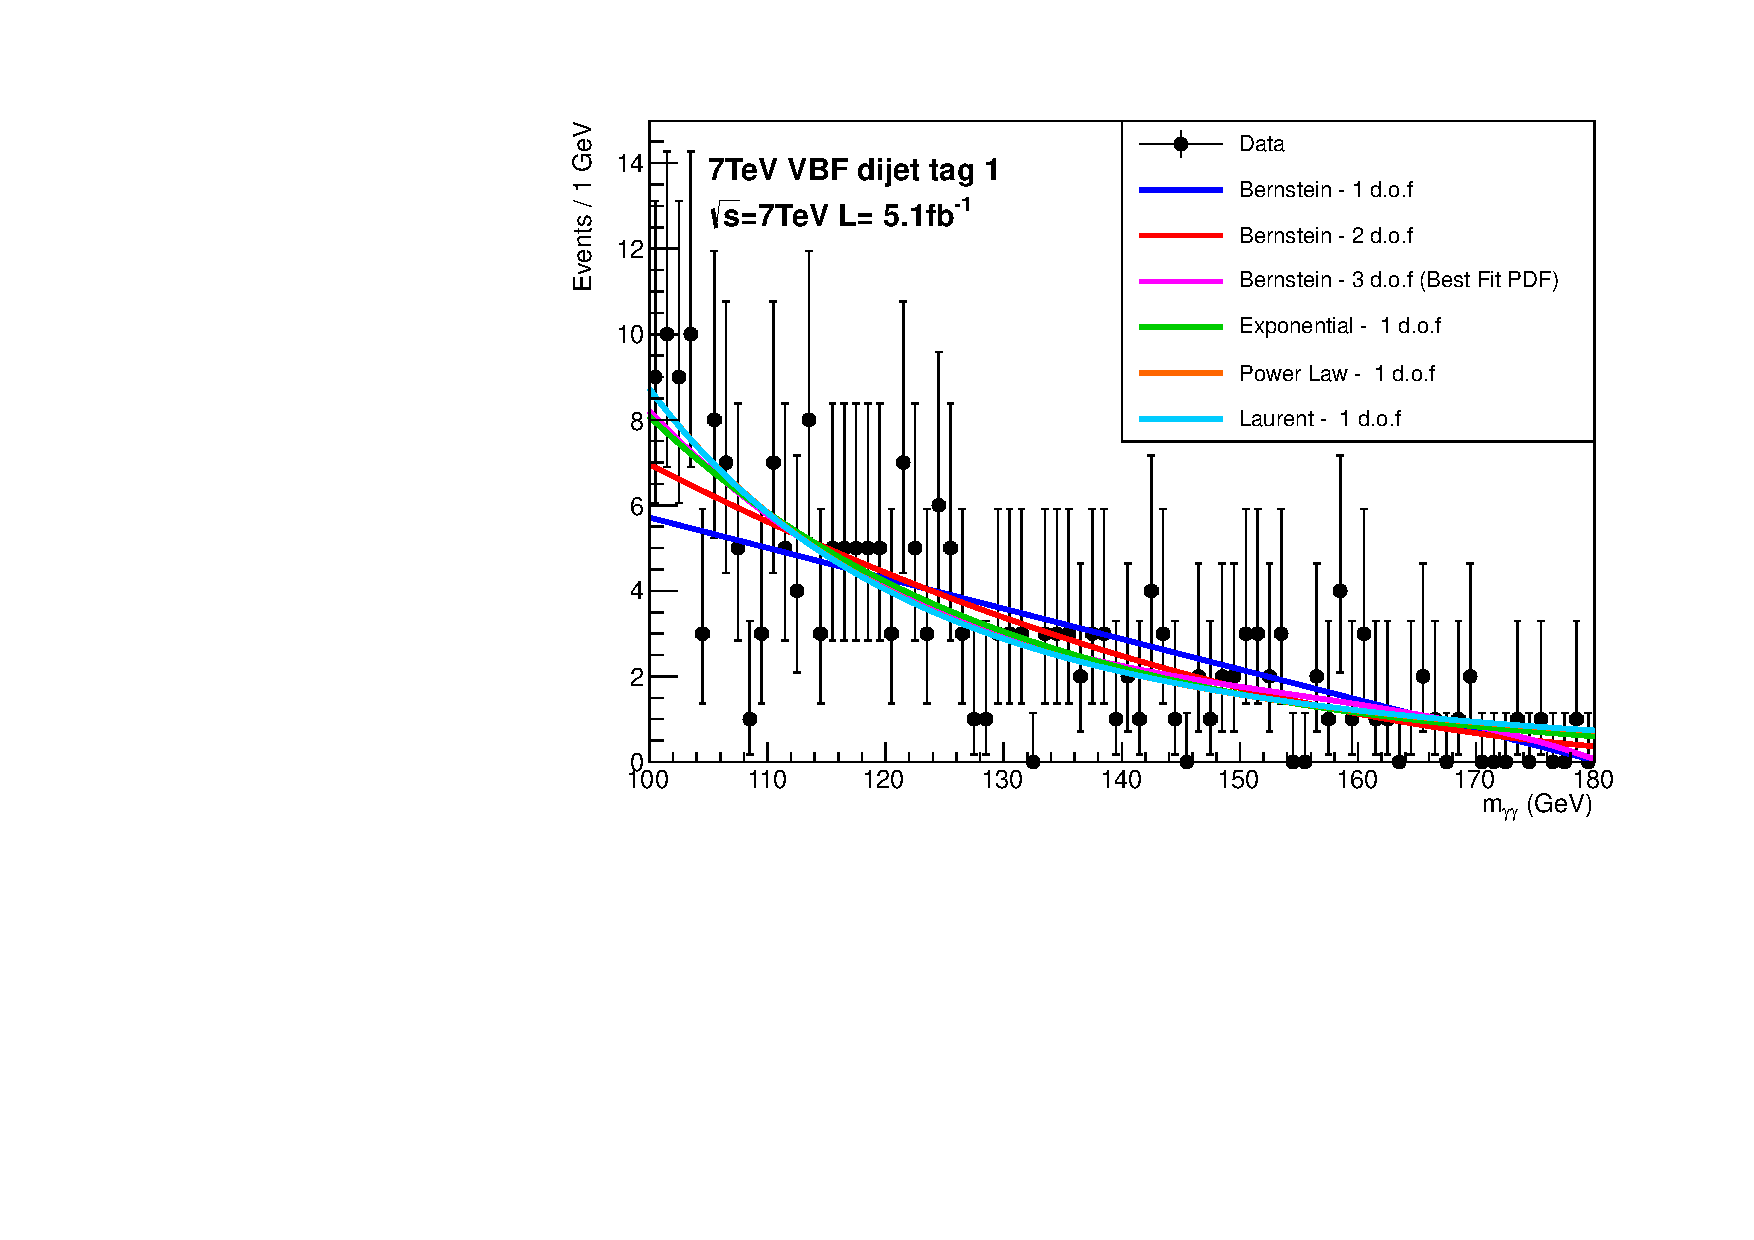
\includegraphics[width=0.49\textwidth]{analysis/plots/multipdf_plots/cat5_7TeV.pdf}\\
  \caption{The diphoton invariant mass distribution and the function choices for the background envelope for the dijet categories in the 7~\TeV dataset.}
  \label{fig:multipdf2}
\end{figure}

\begin{figure}
  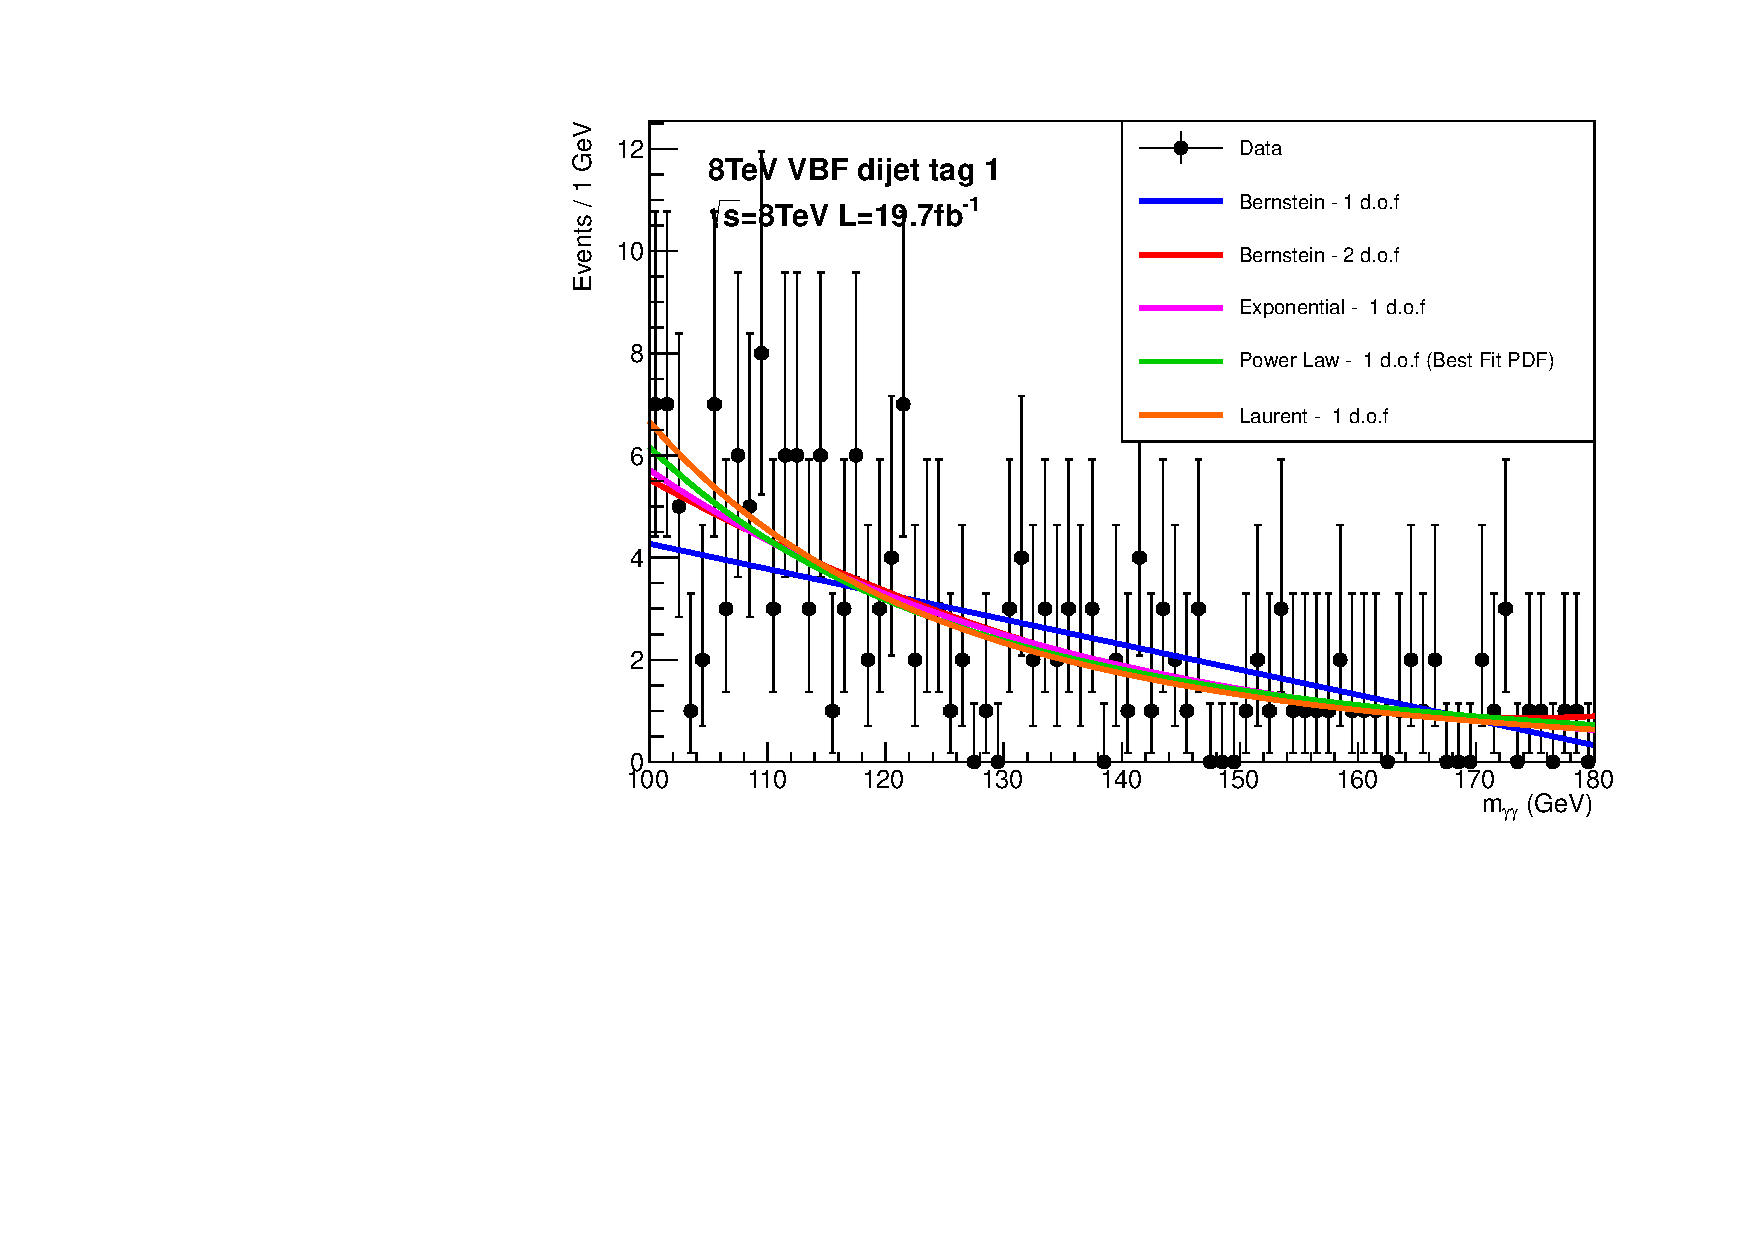
\includegraphics[width=0.49\textwidth]{analysis/plots/multipdf_plots/cat6_8TeV.pdf}
  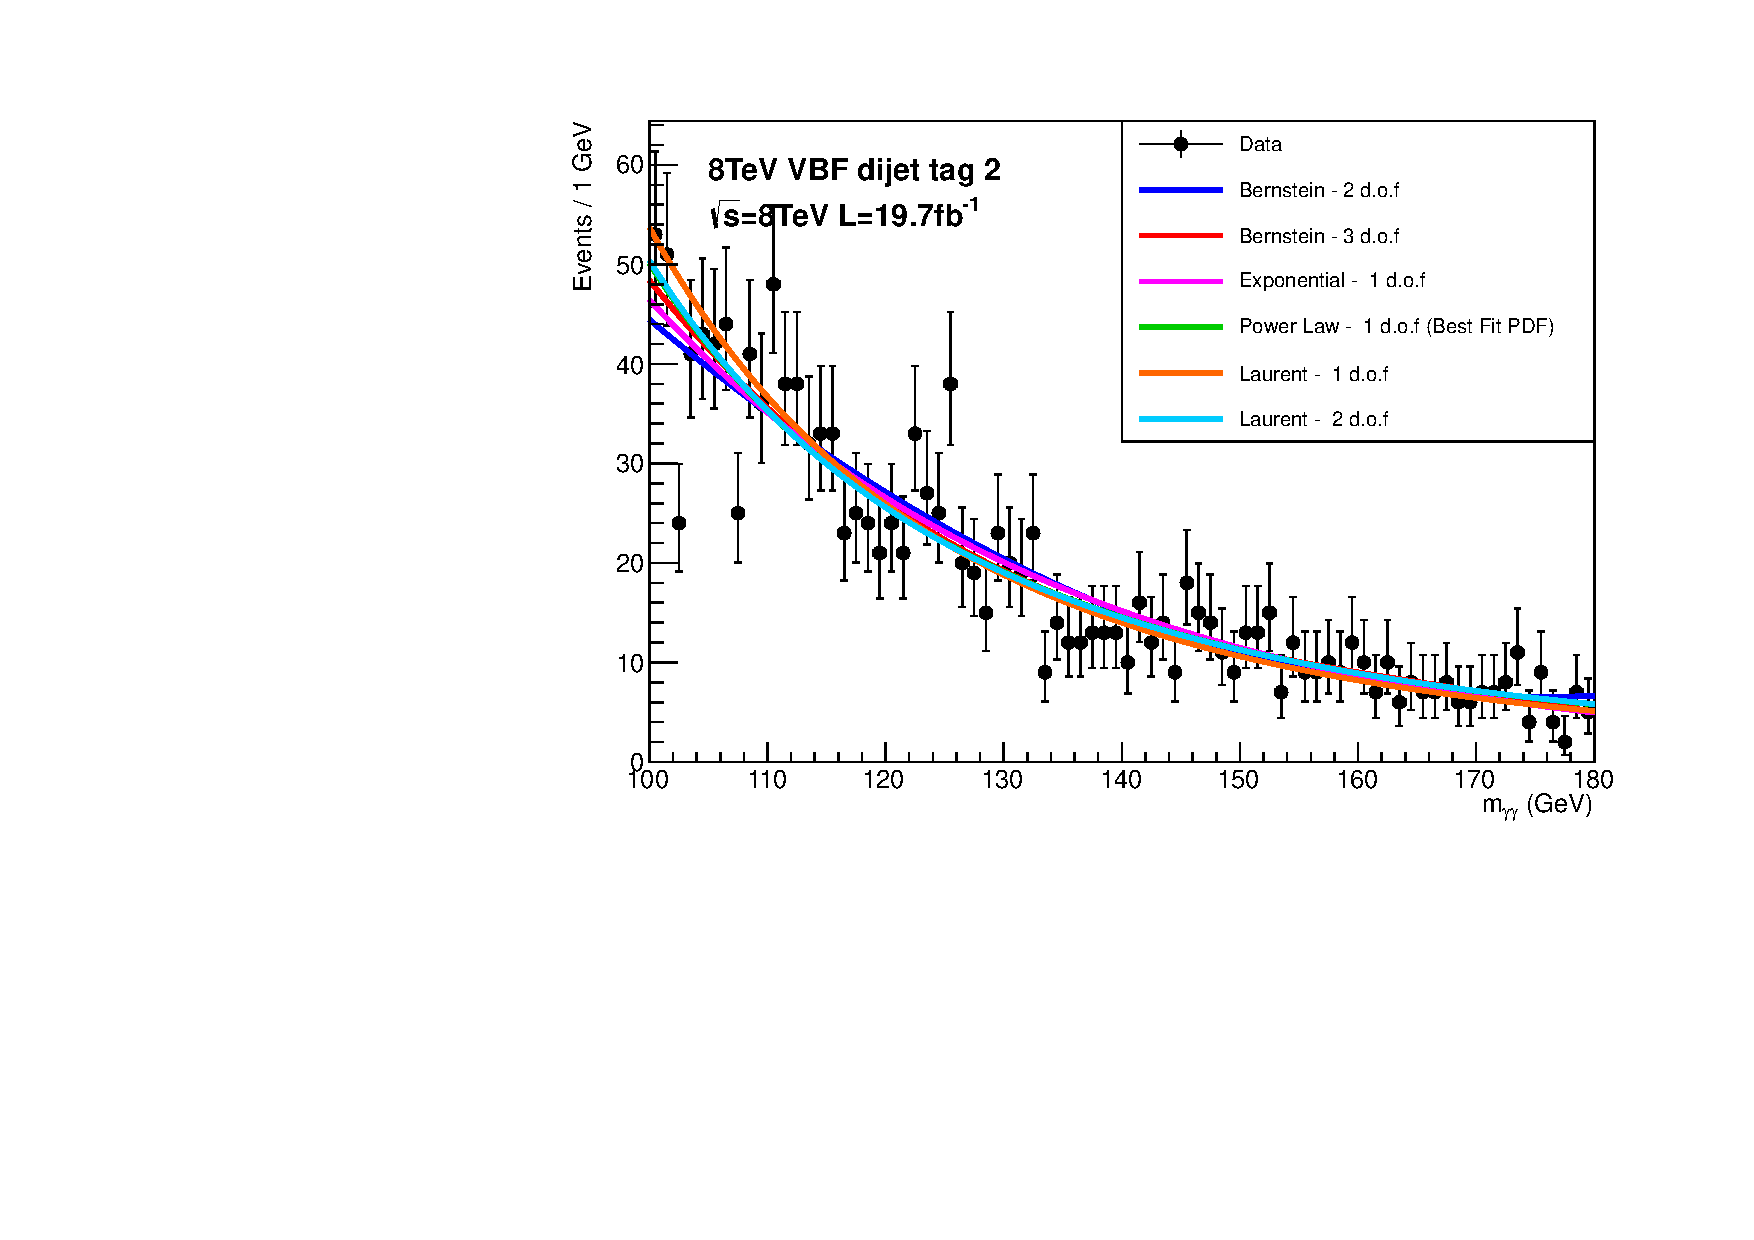
\includegraphics[width=0.49\textwidth]{analysis/plots/multipdf_plots/cat7_8TeV.pdf}\\
  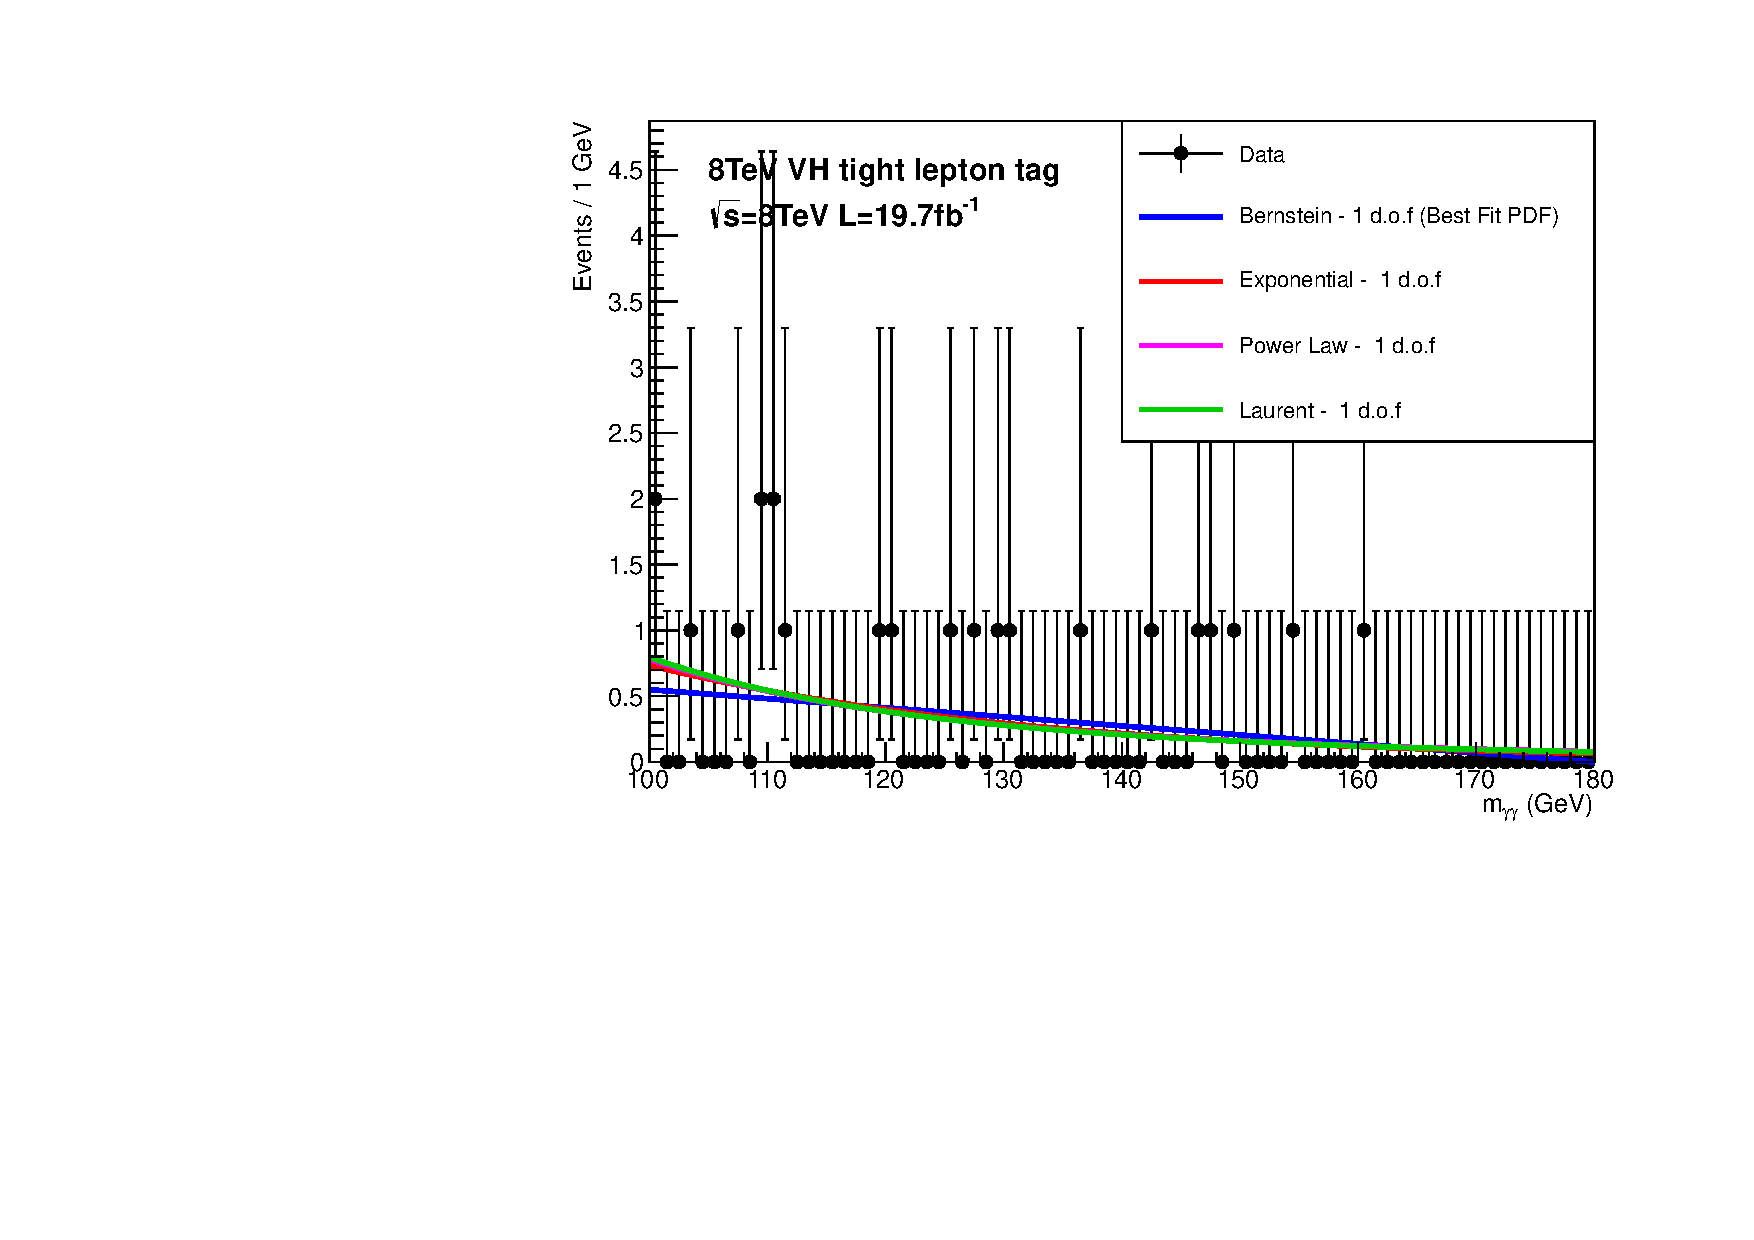
\includegraphics[width=0.49\textwidth]{analysis/plots/multipdf_plots/cat8_8TeV.pdf}
  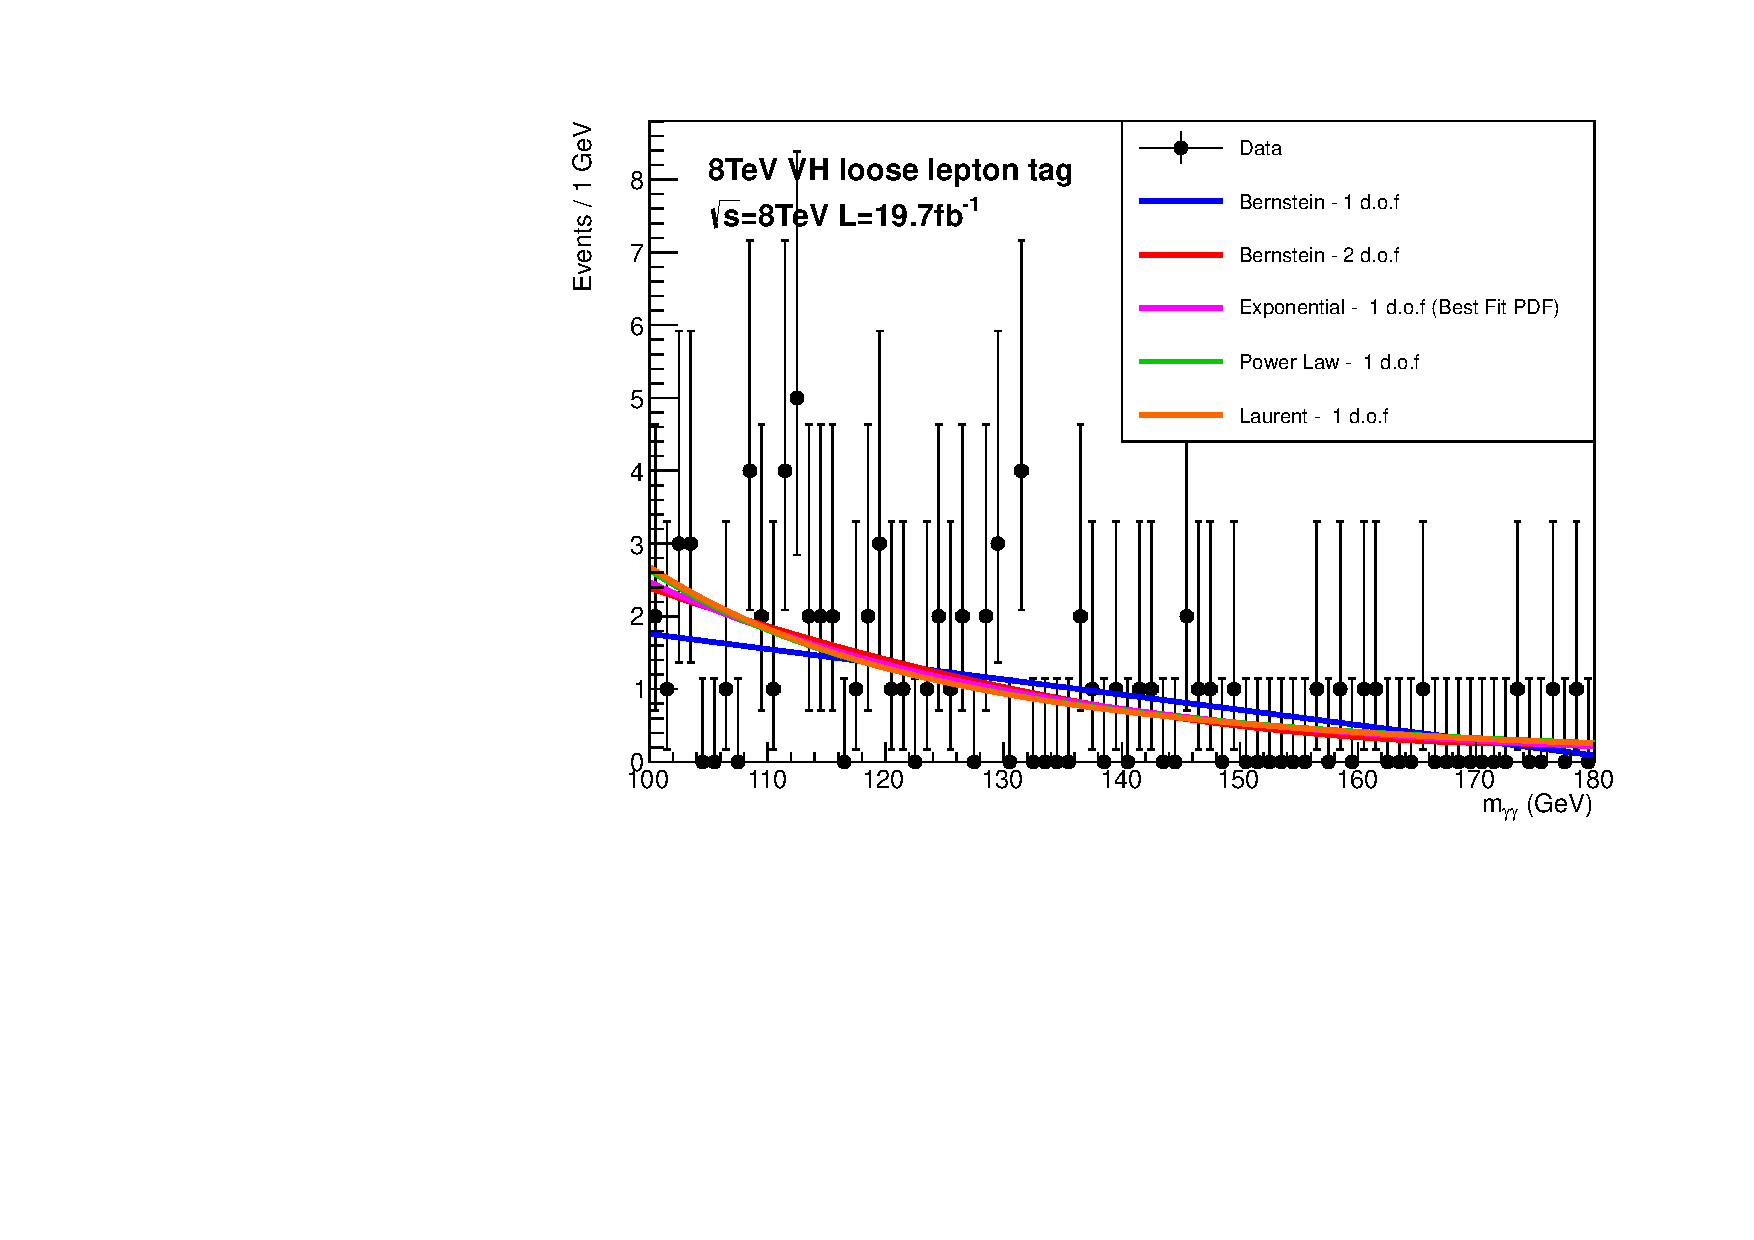
\includegraphics[width=0.49\textwidth]{analysis/plots/multipdf_plots/cat9_8TeV.pdf}\\
  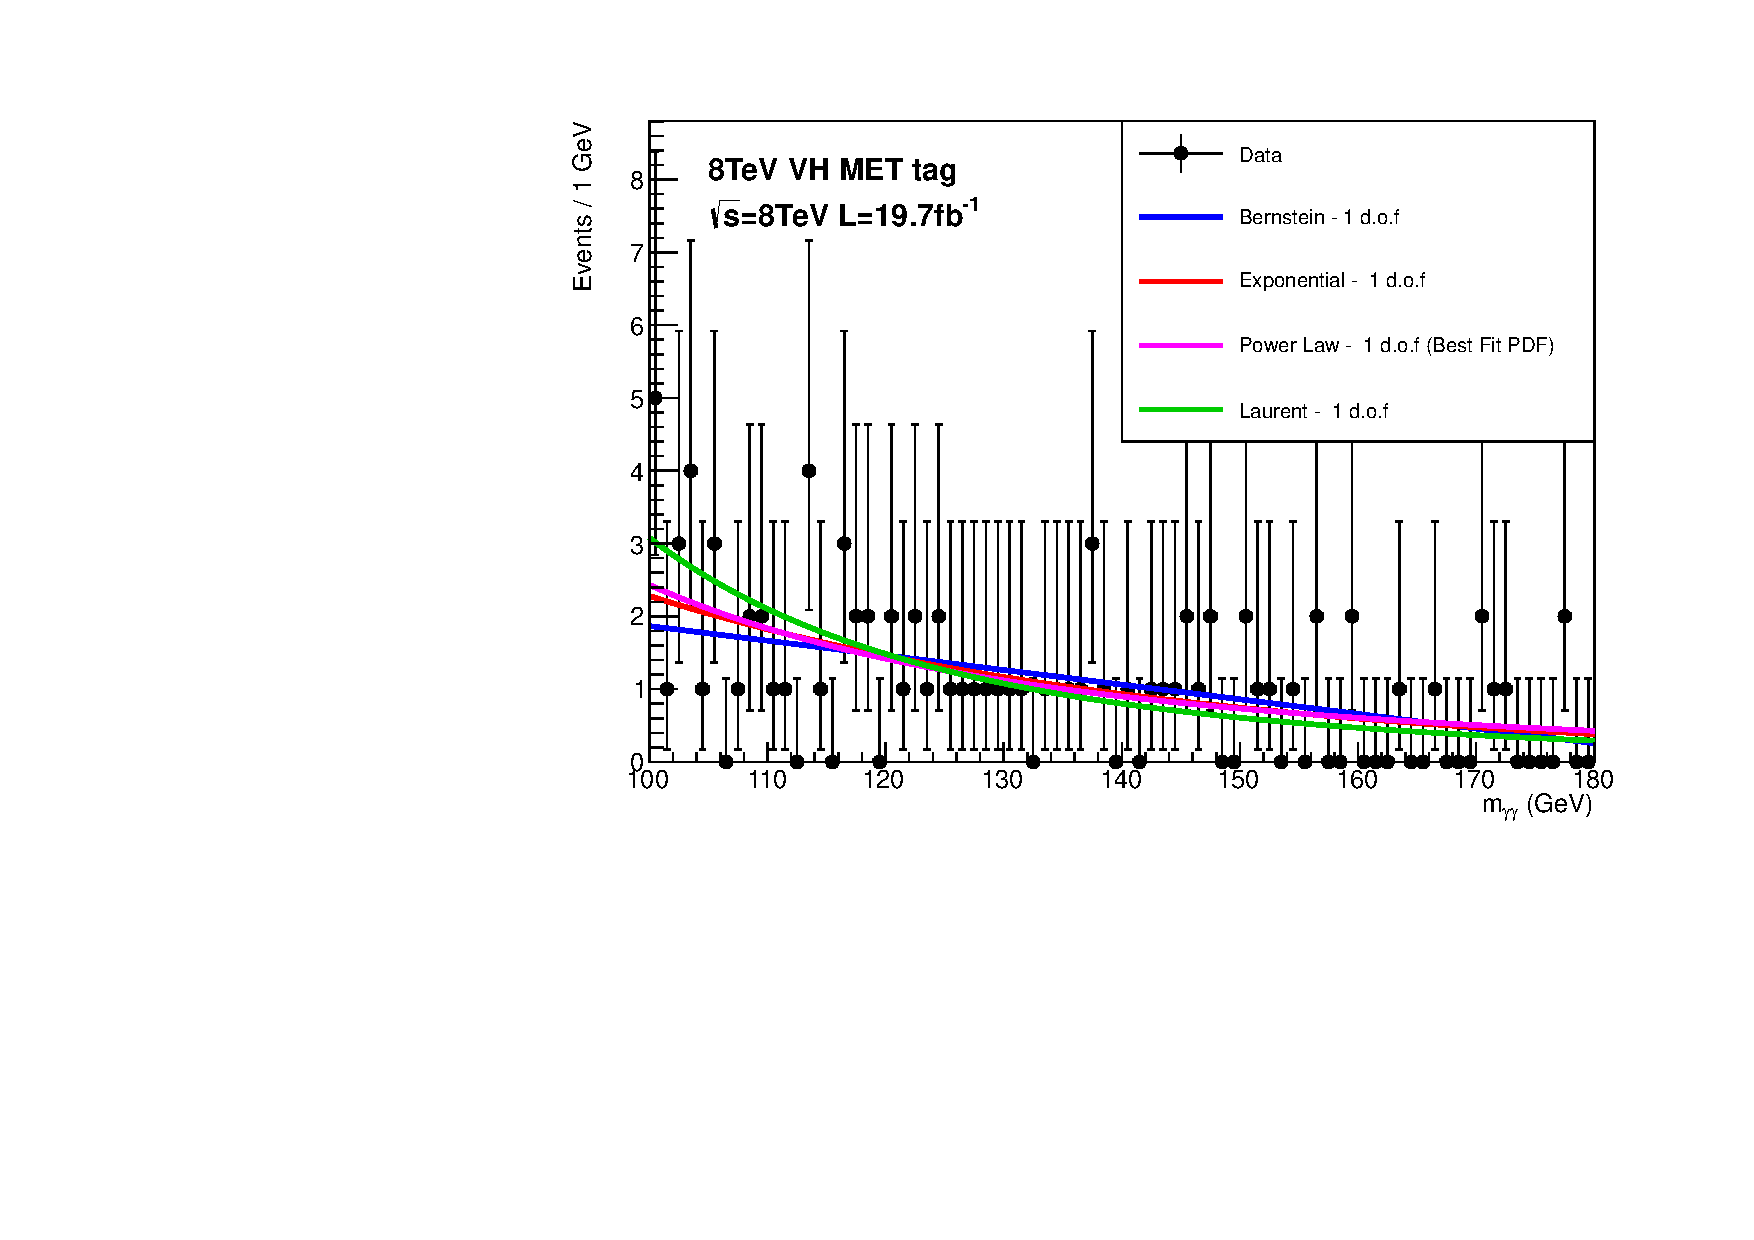
\includegraphics[width=0.49\textwidth]{analysis/plots/multipdf_plots/cat10_8TeV.pdf}
  \caption{The diphoton invariant mass distribution and the function choices for the background envelope for the \VH and \ttH categories in the 7~\TeV dataset.}
  \label{fig:multipdf3}
\end{figure}

\begin{figure}
  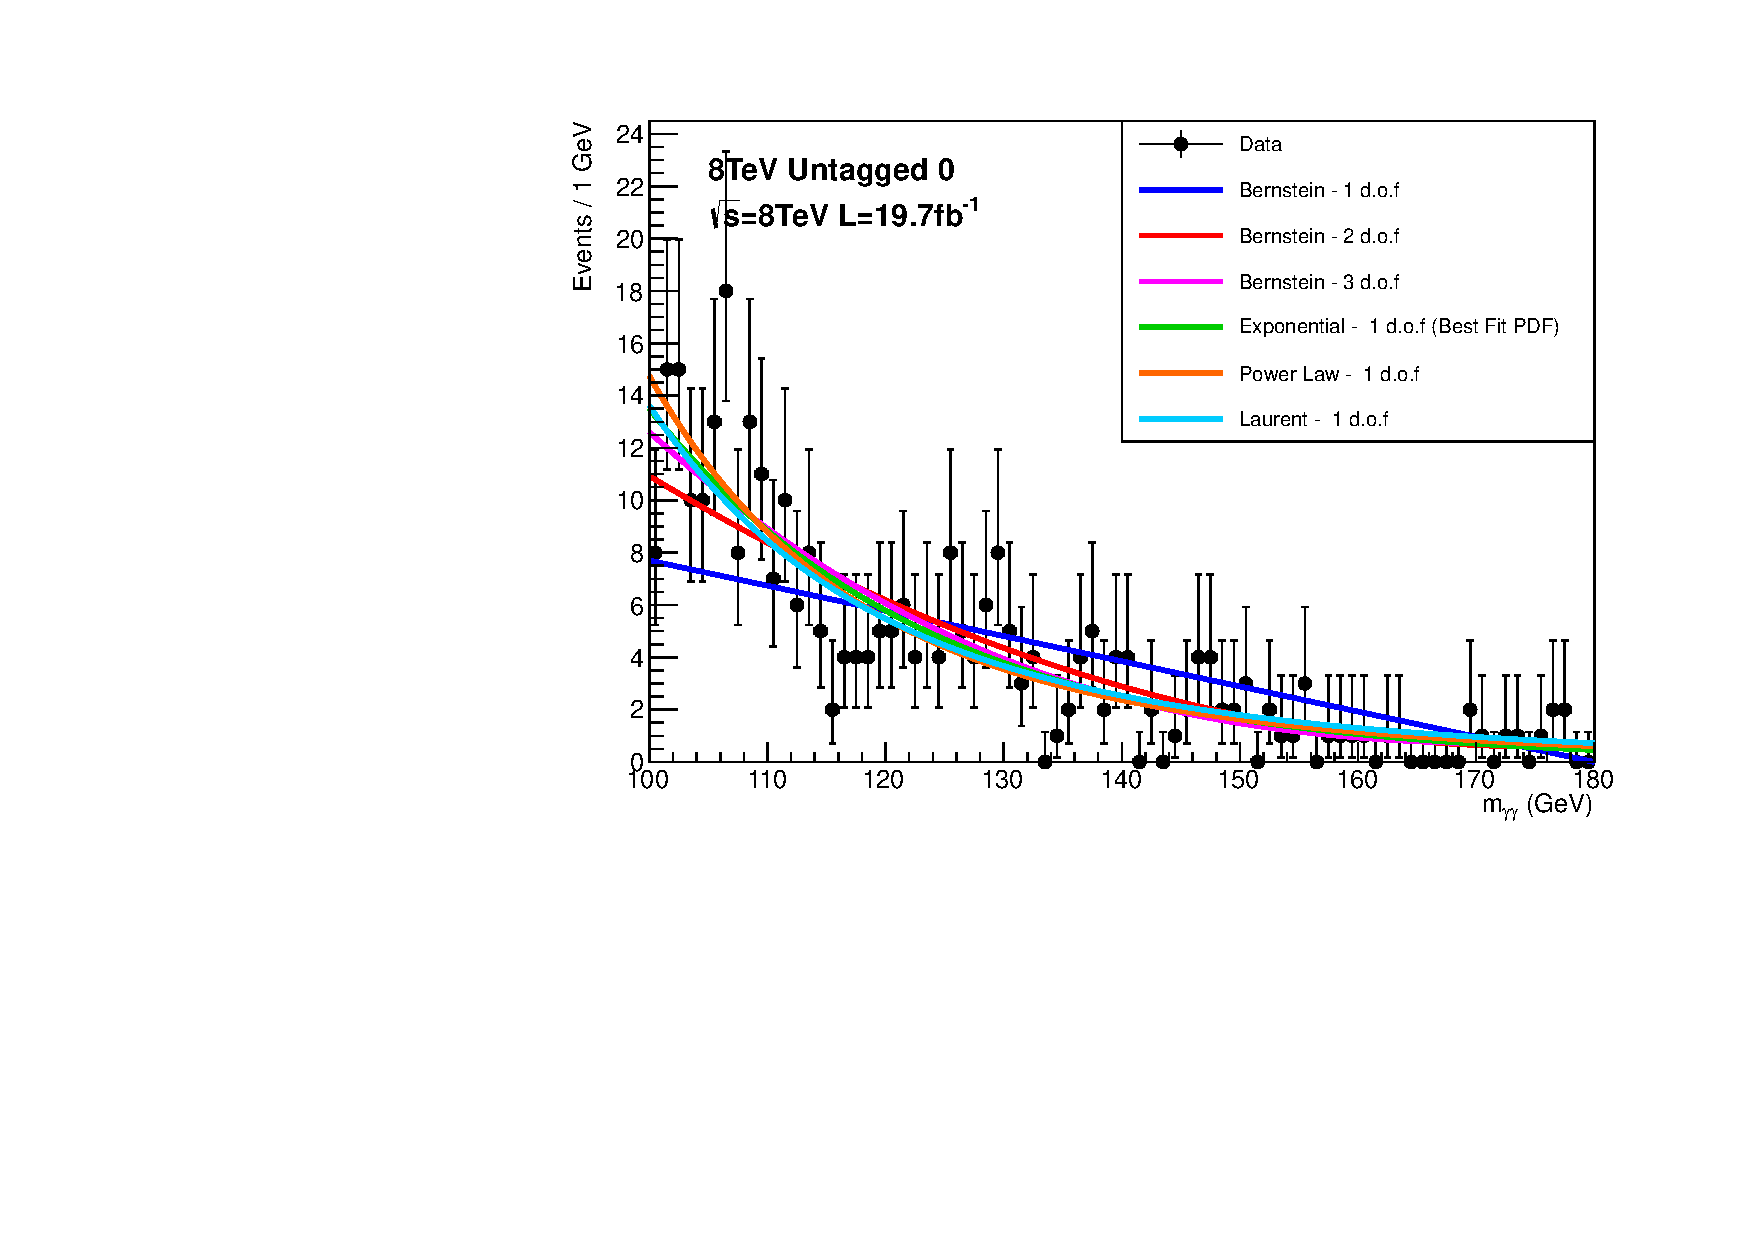
\includegraphics[width=0.49\textwidth]{analysis/plots/multipdf_plots/cat0_8TeV.pdf}
  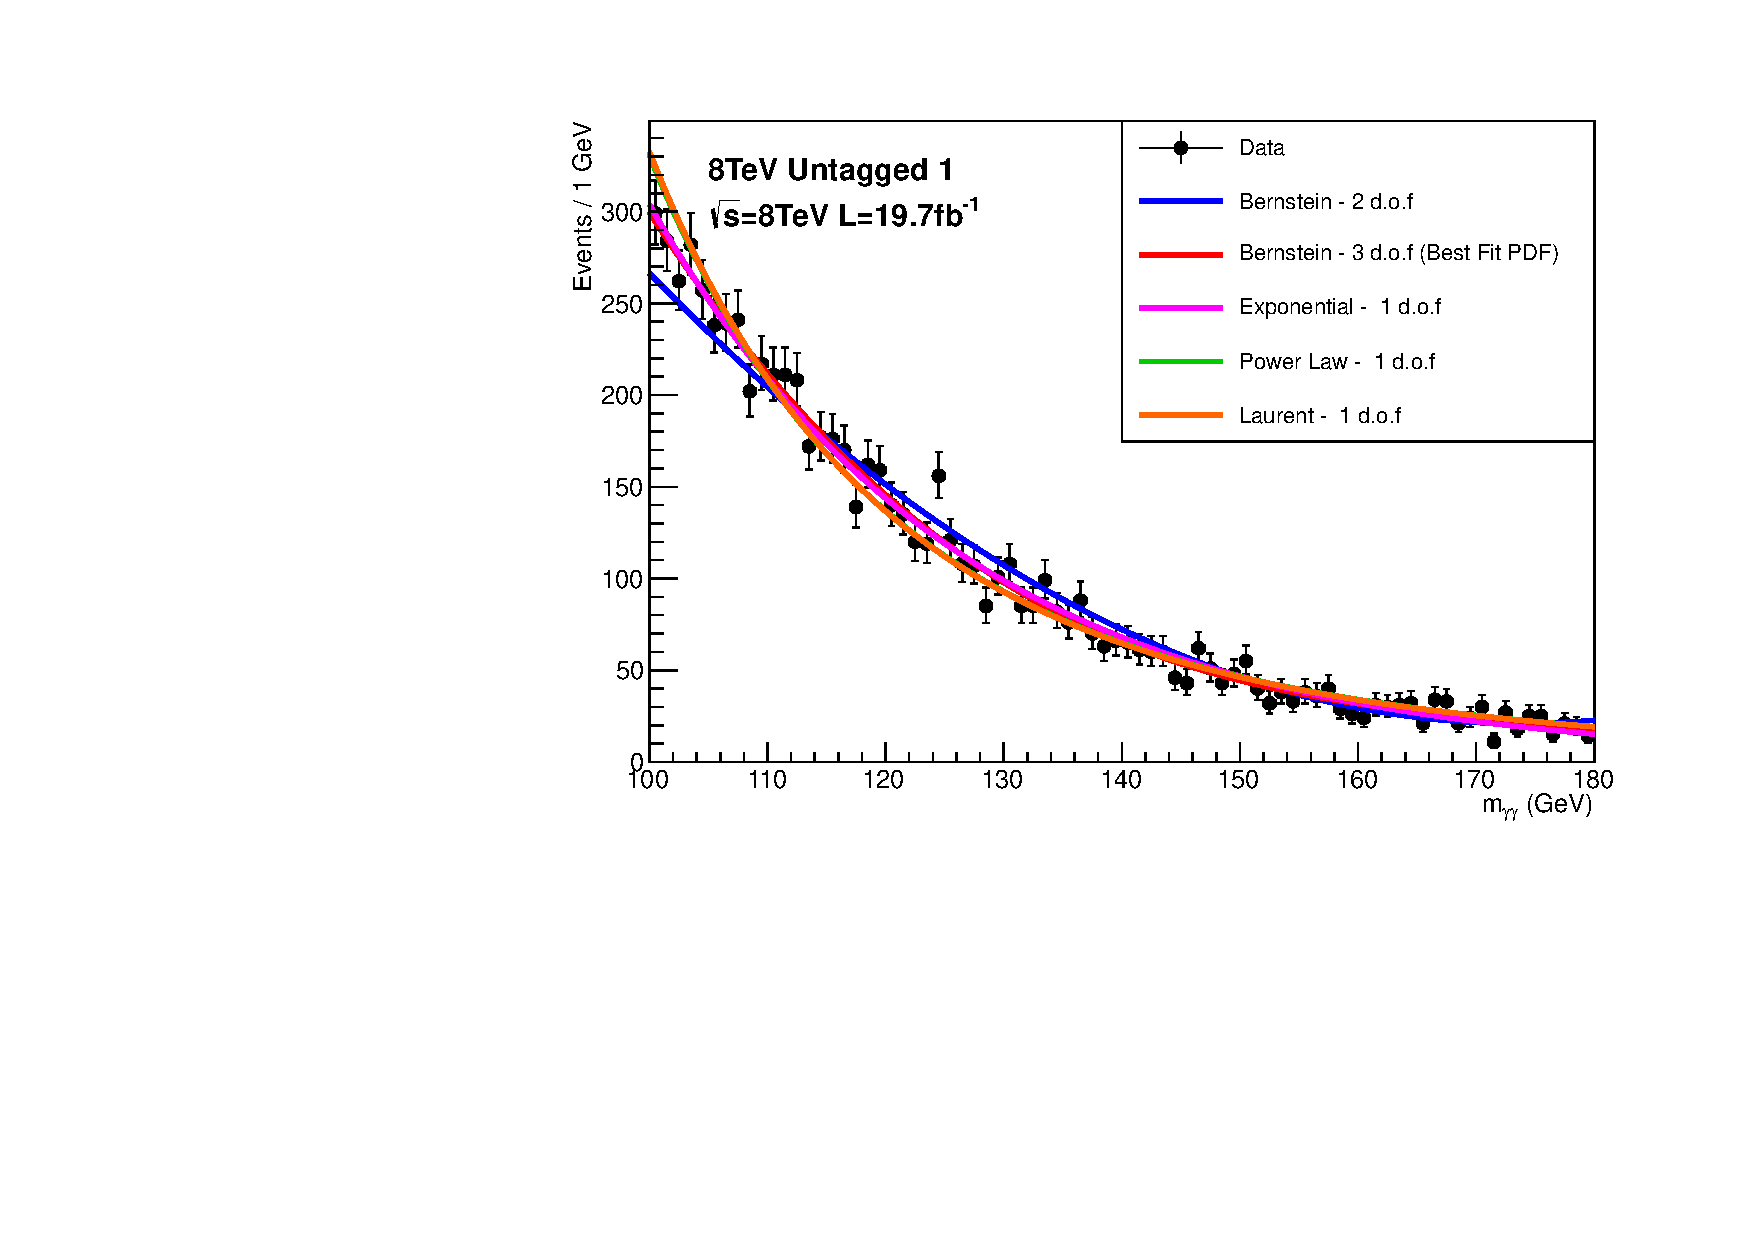
\includegraphics[width=0.49\textwidth]{analysis/plots/multipdf_plots/cat1_8TeV.pdf}\\
  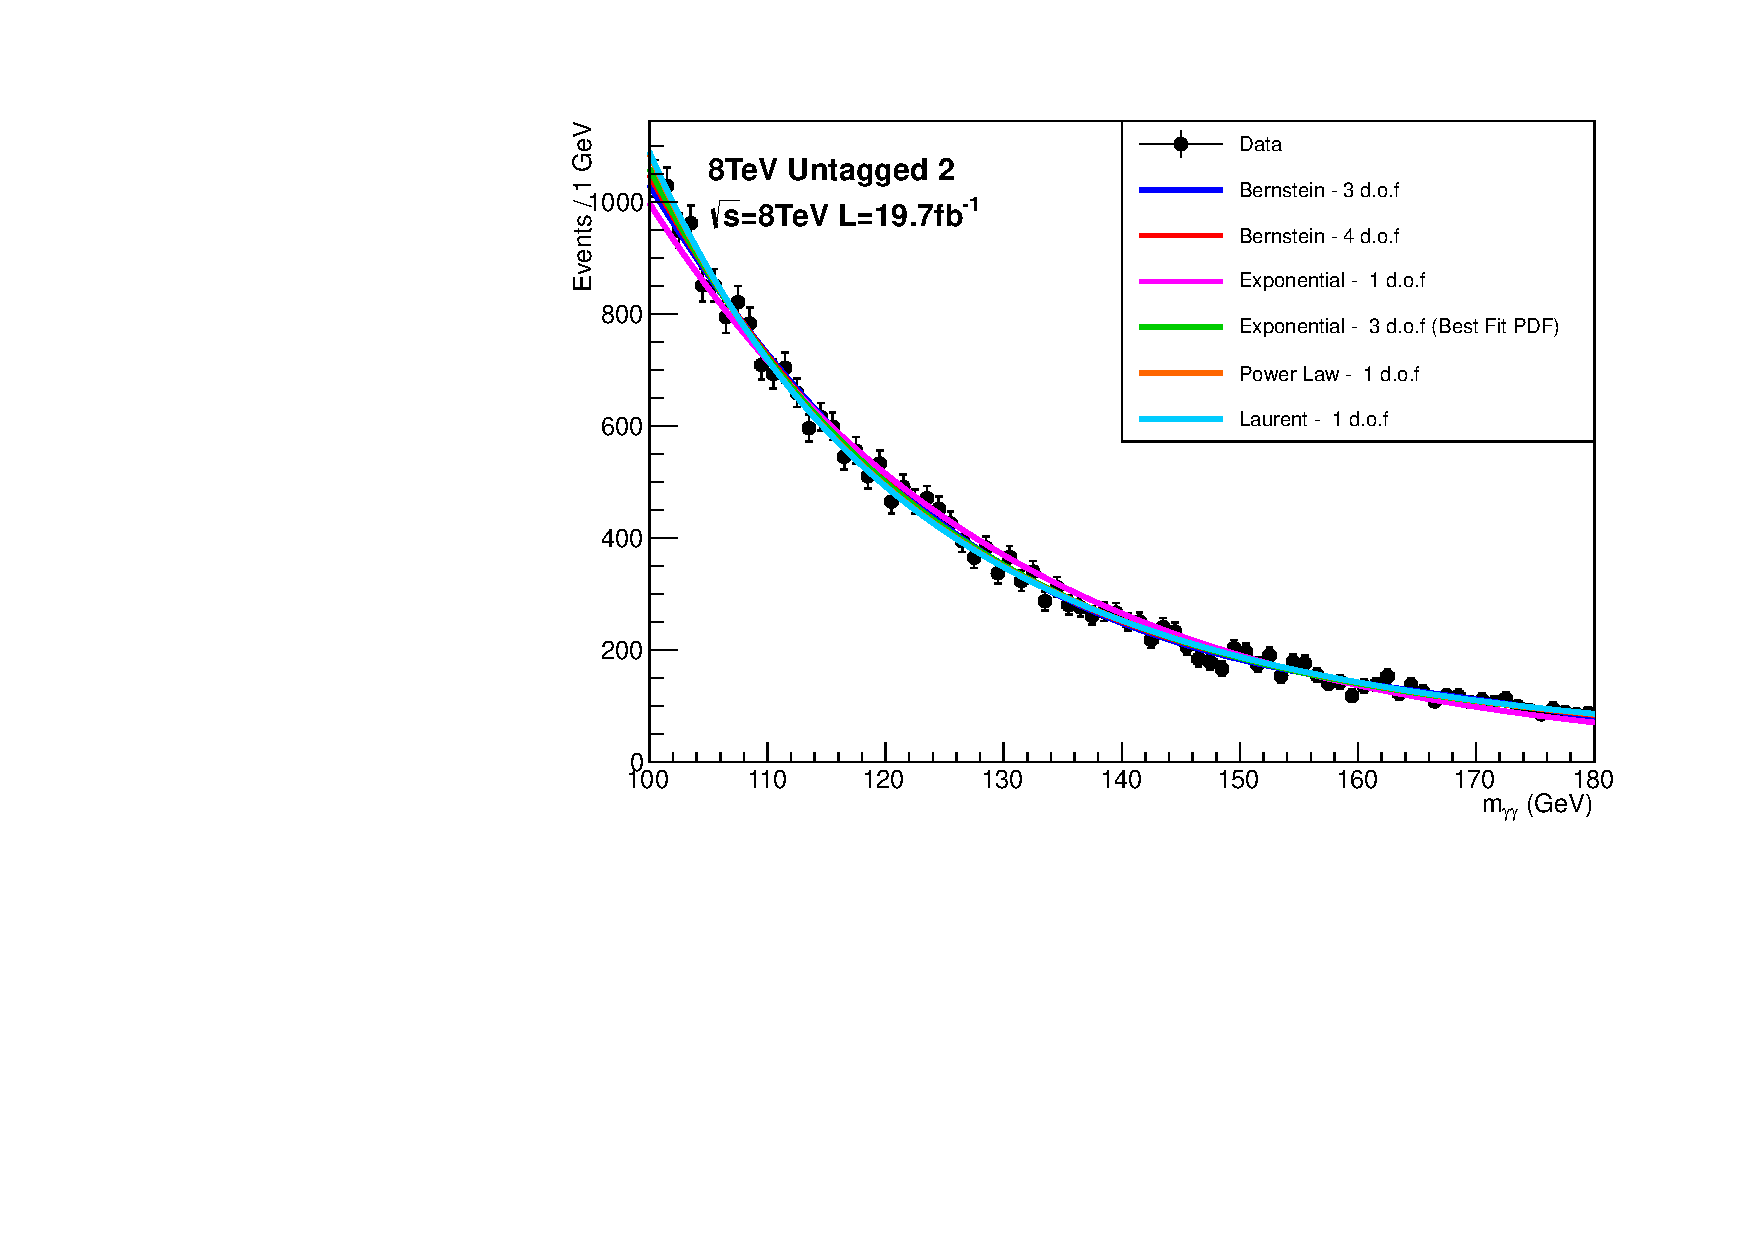
\includegraphics[width=0.49\textwidth]{analysis/plots/multipdf_plots/cat2_8TeV.pdf}
  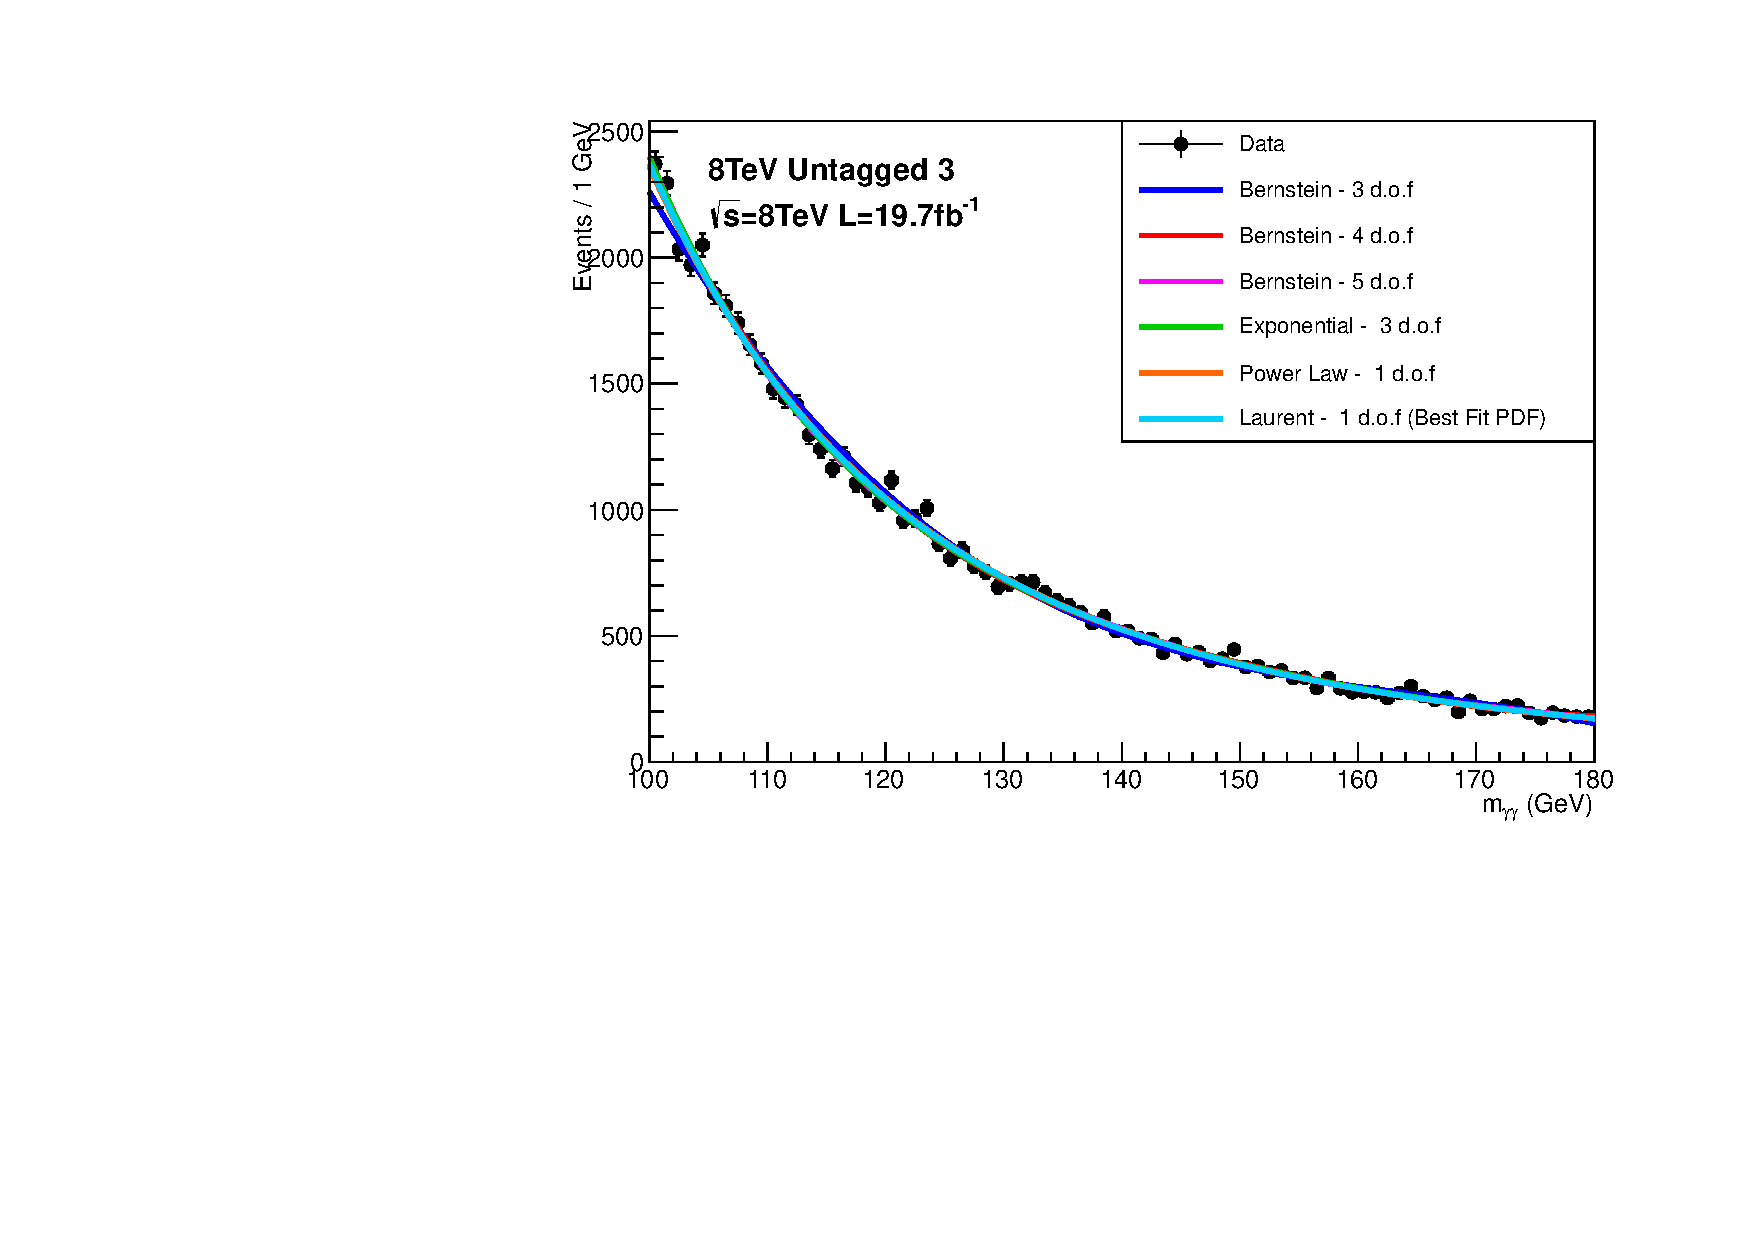
\includegraphics[width=0.49\textwidth]{analysis/plots/multipdf_plots/cat3_8TeV.pdf}\\
  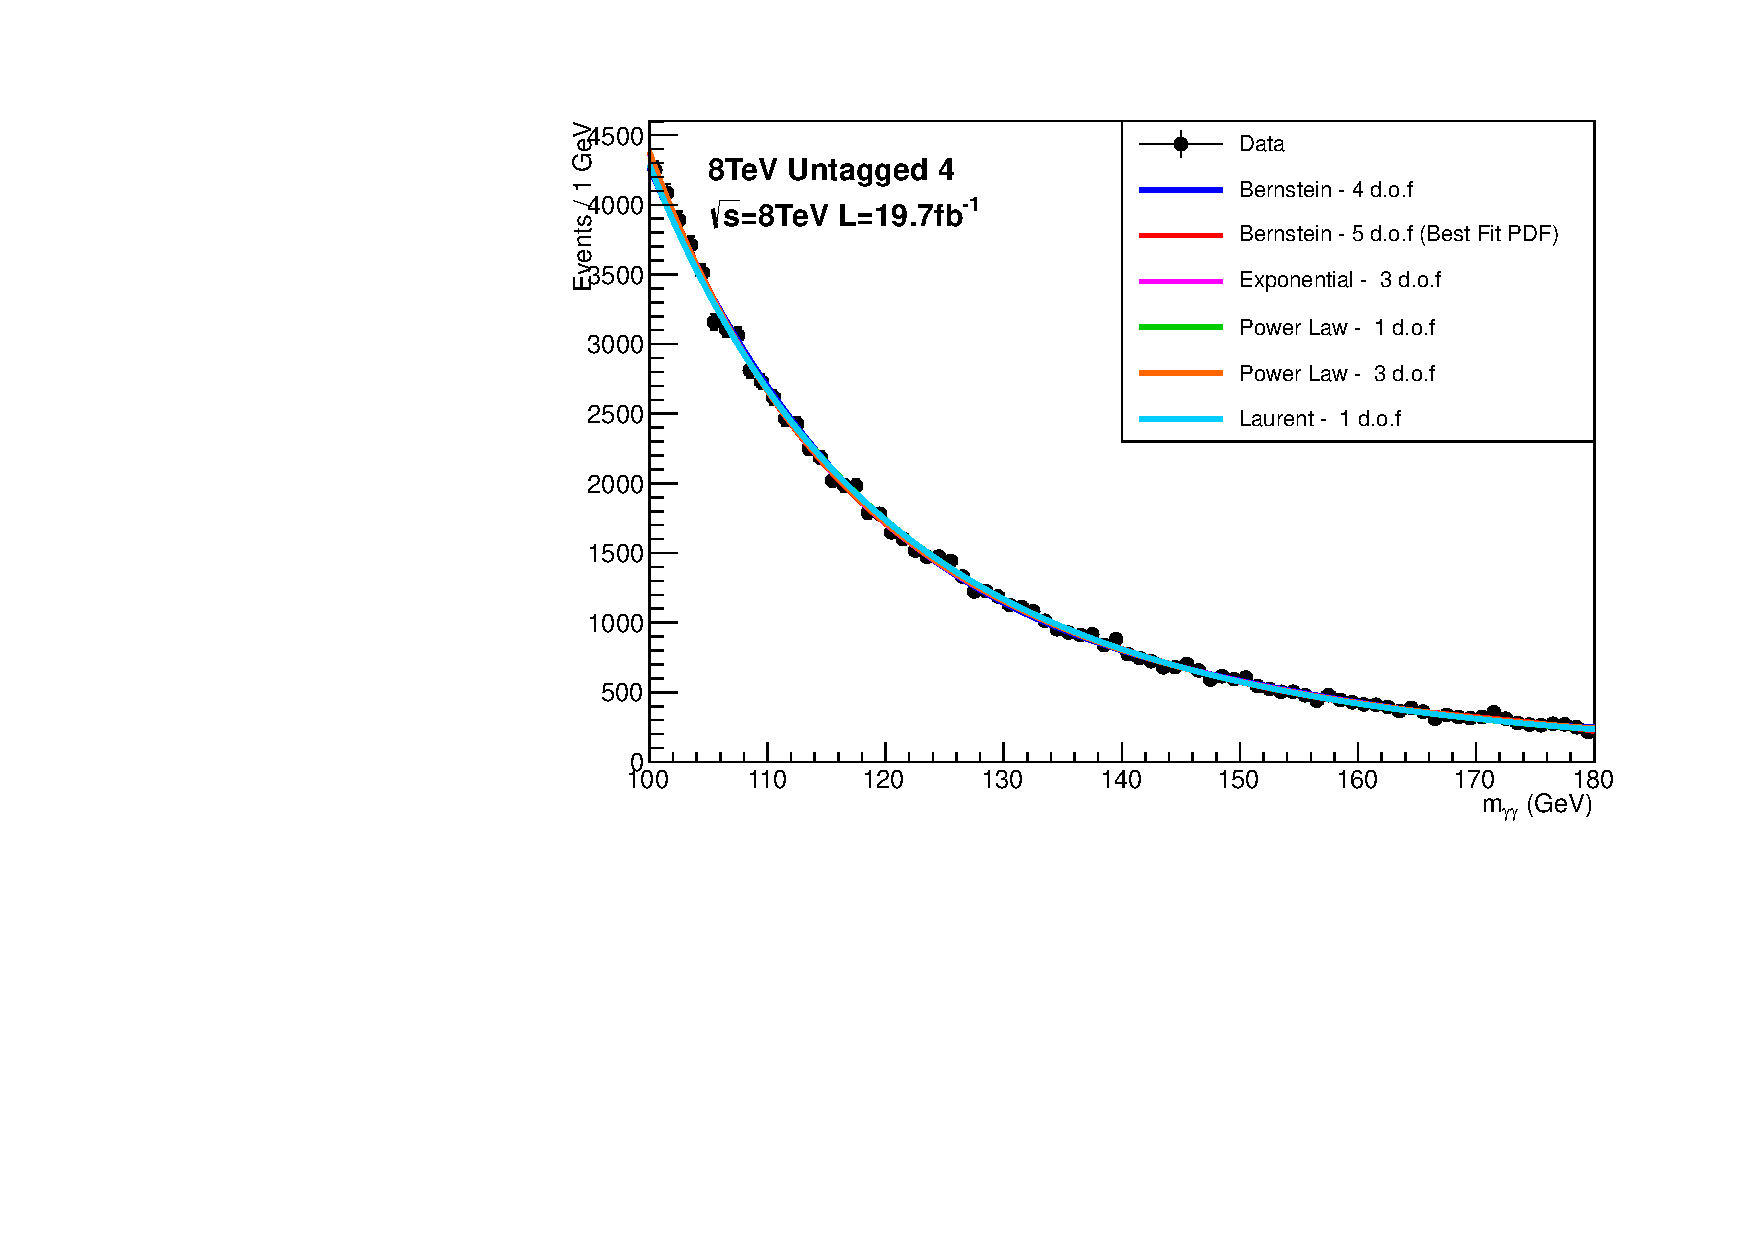
\includegraphics[width=0.49\textwidth]{analysis/plots/multipdf_plots/cat4_8TeV.pdf}
  \caption{The diphoton invariant mass distribution and the function choices for the background envelope for the inclusive categories in the 8~\TeV dataset.}
  \label{fig:multipdf4}
\end{figure}

\begin{figure}
  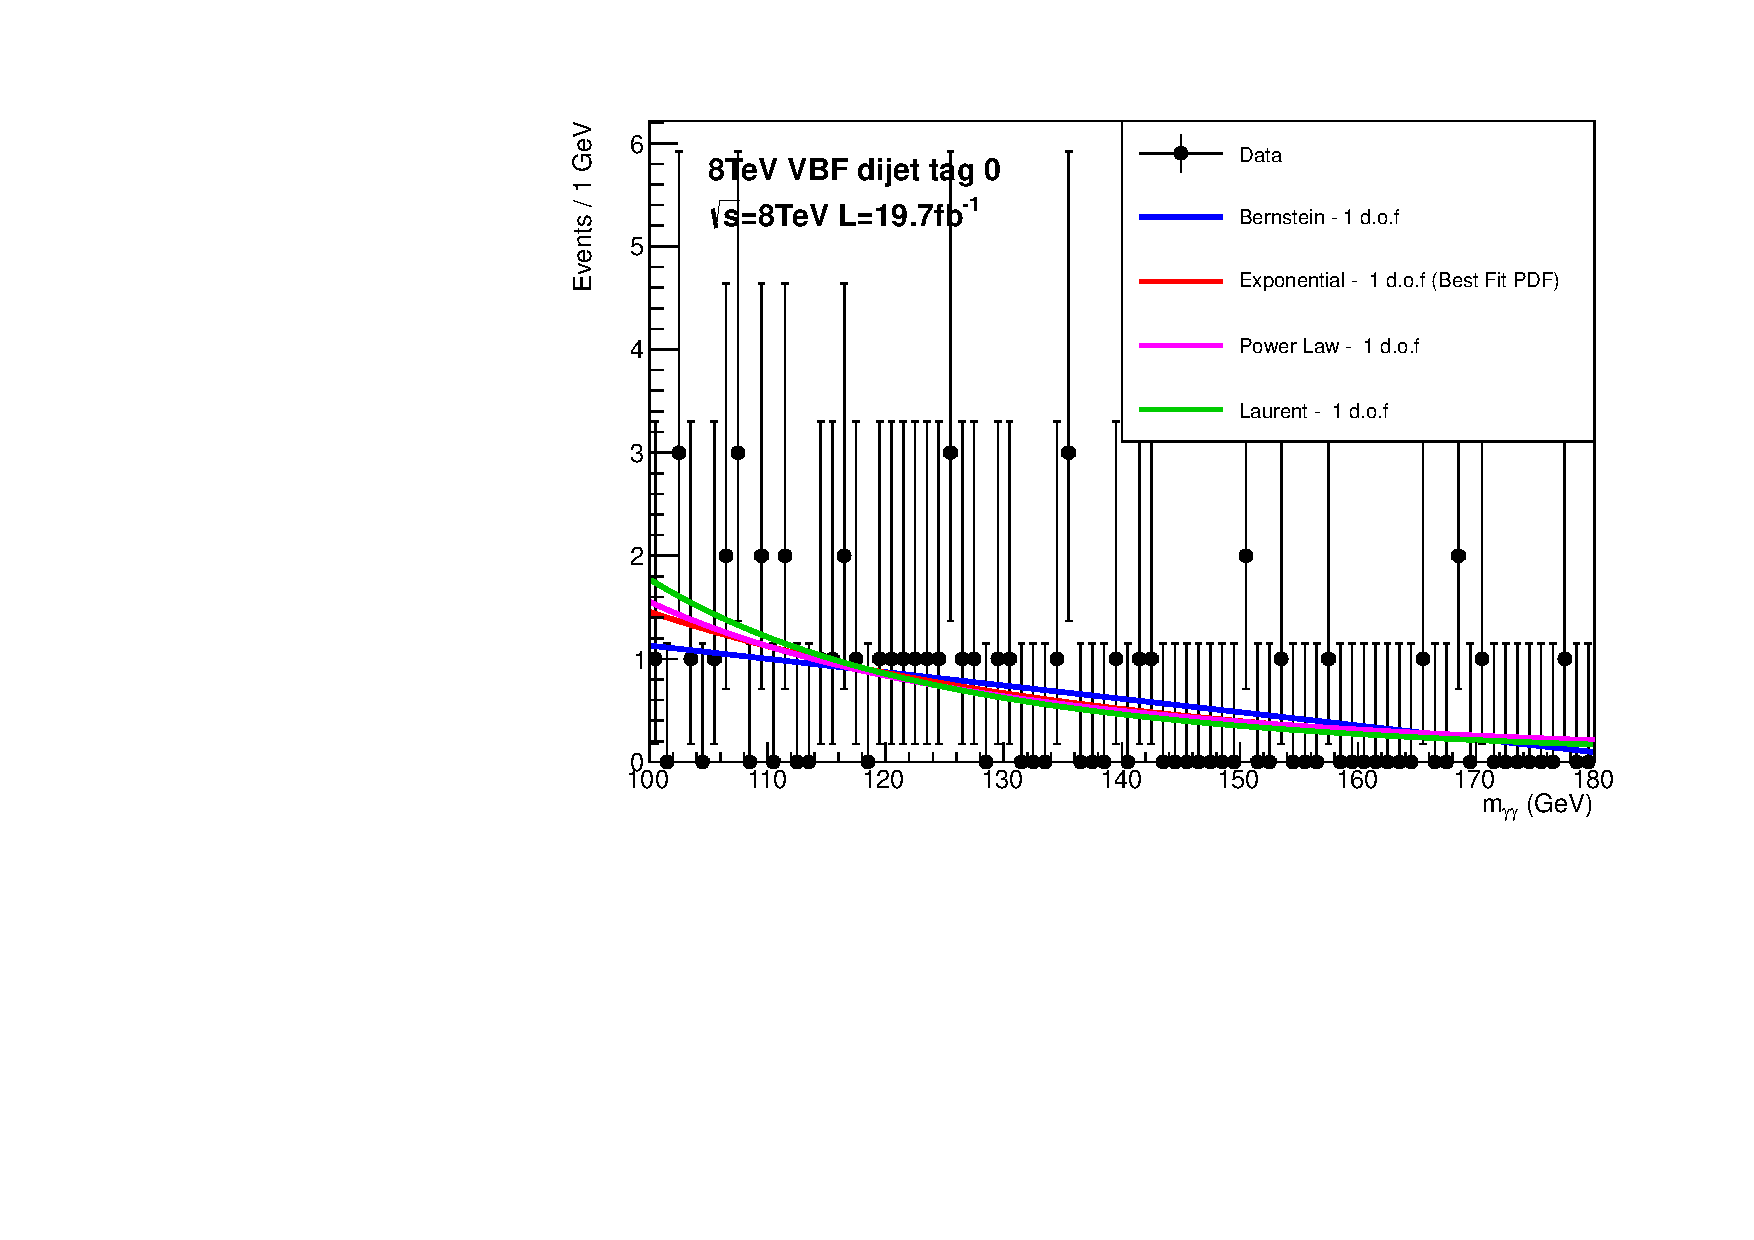
\includegraphics[width=0.49\textwidth]{analysis/plots/multipdf_plots/cat5_8TeV.pdf}
  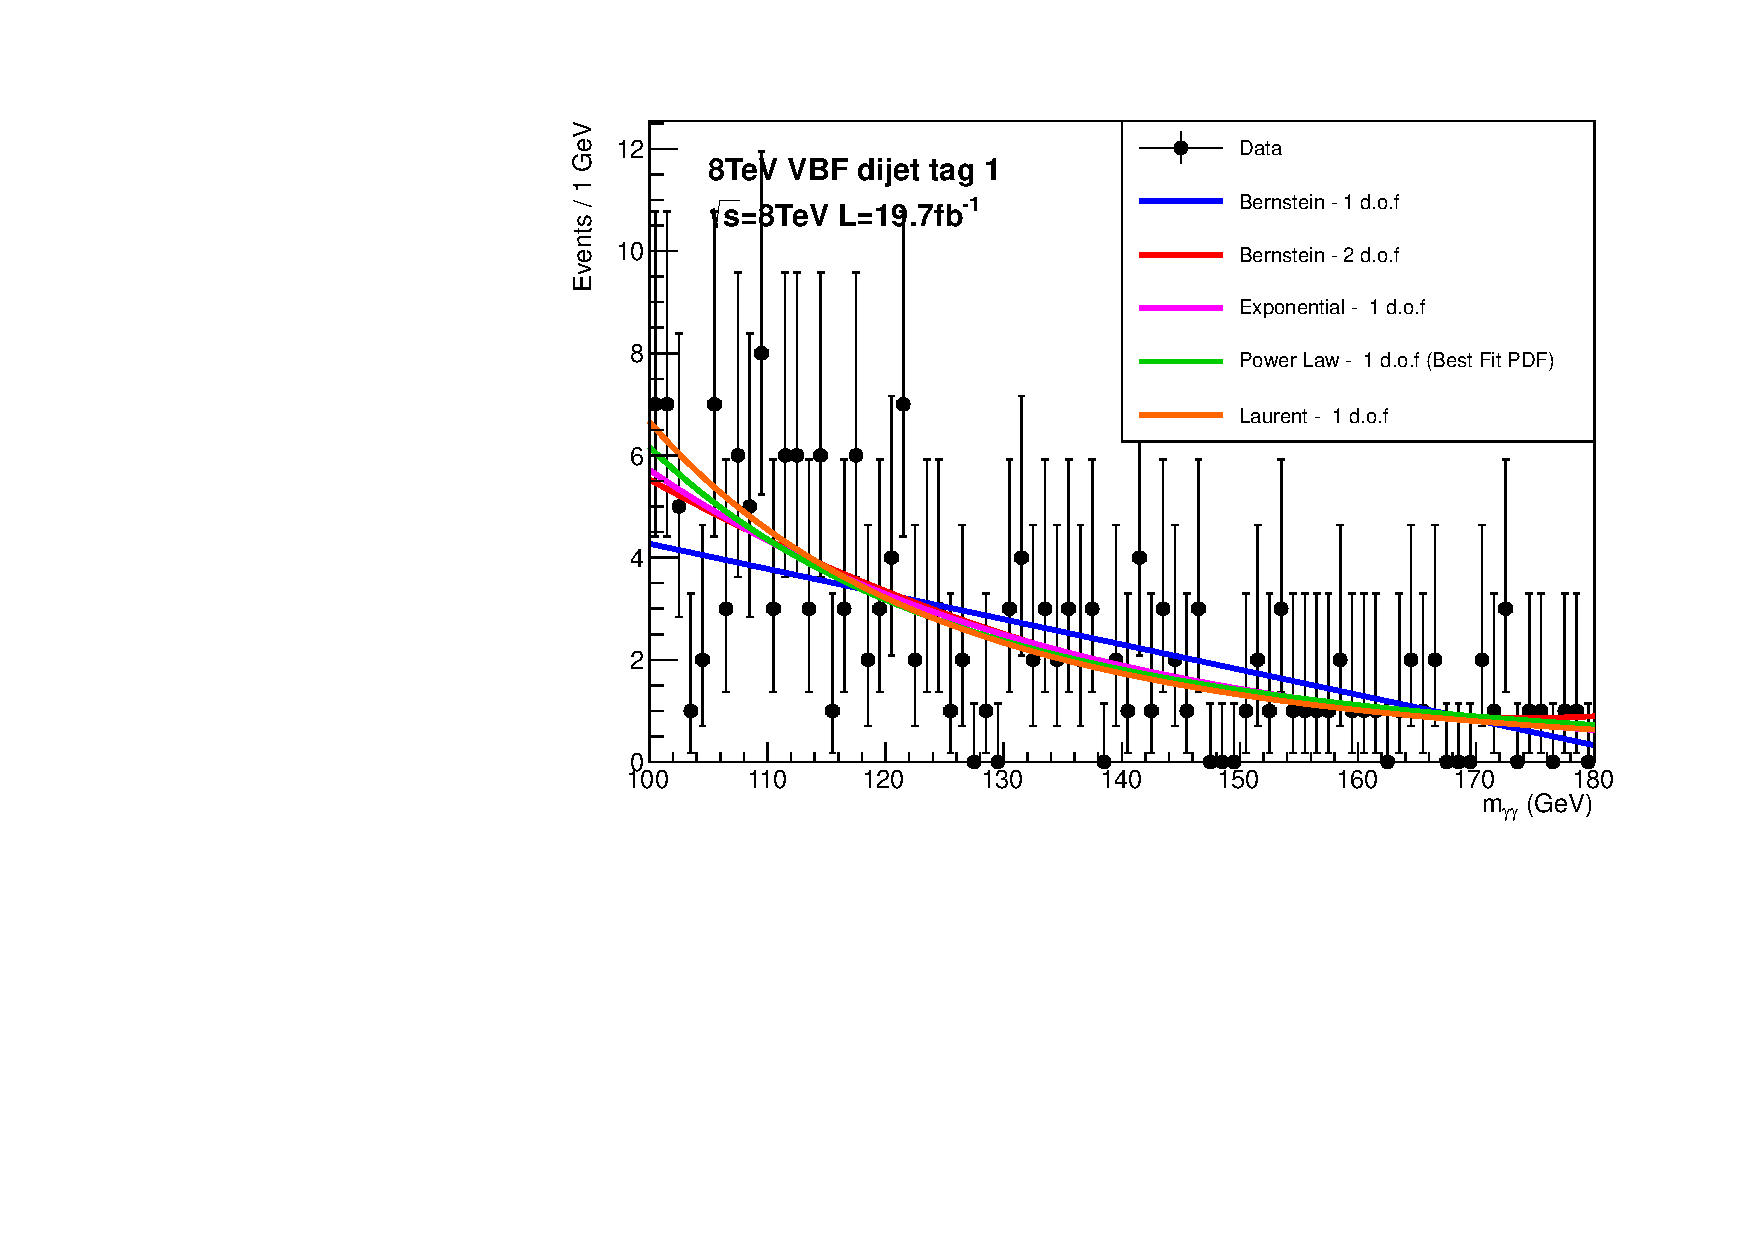
\includegraphics[width=0.49\textwidth]{analysis/plots/multipdf_plots/cat6_8TeV.pdf}\\
  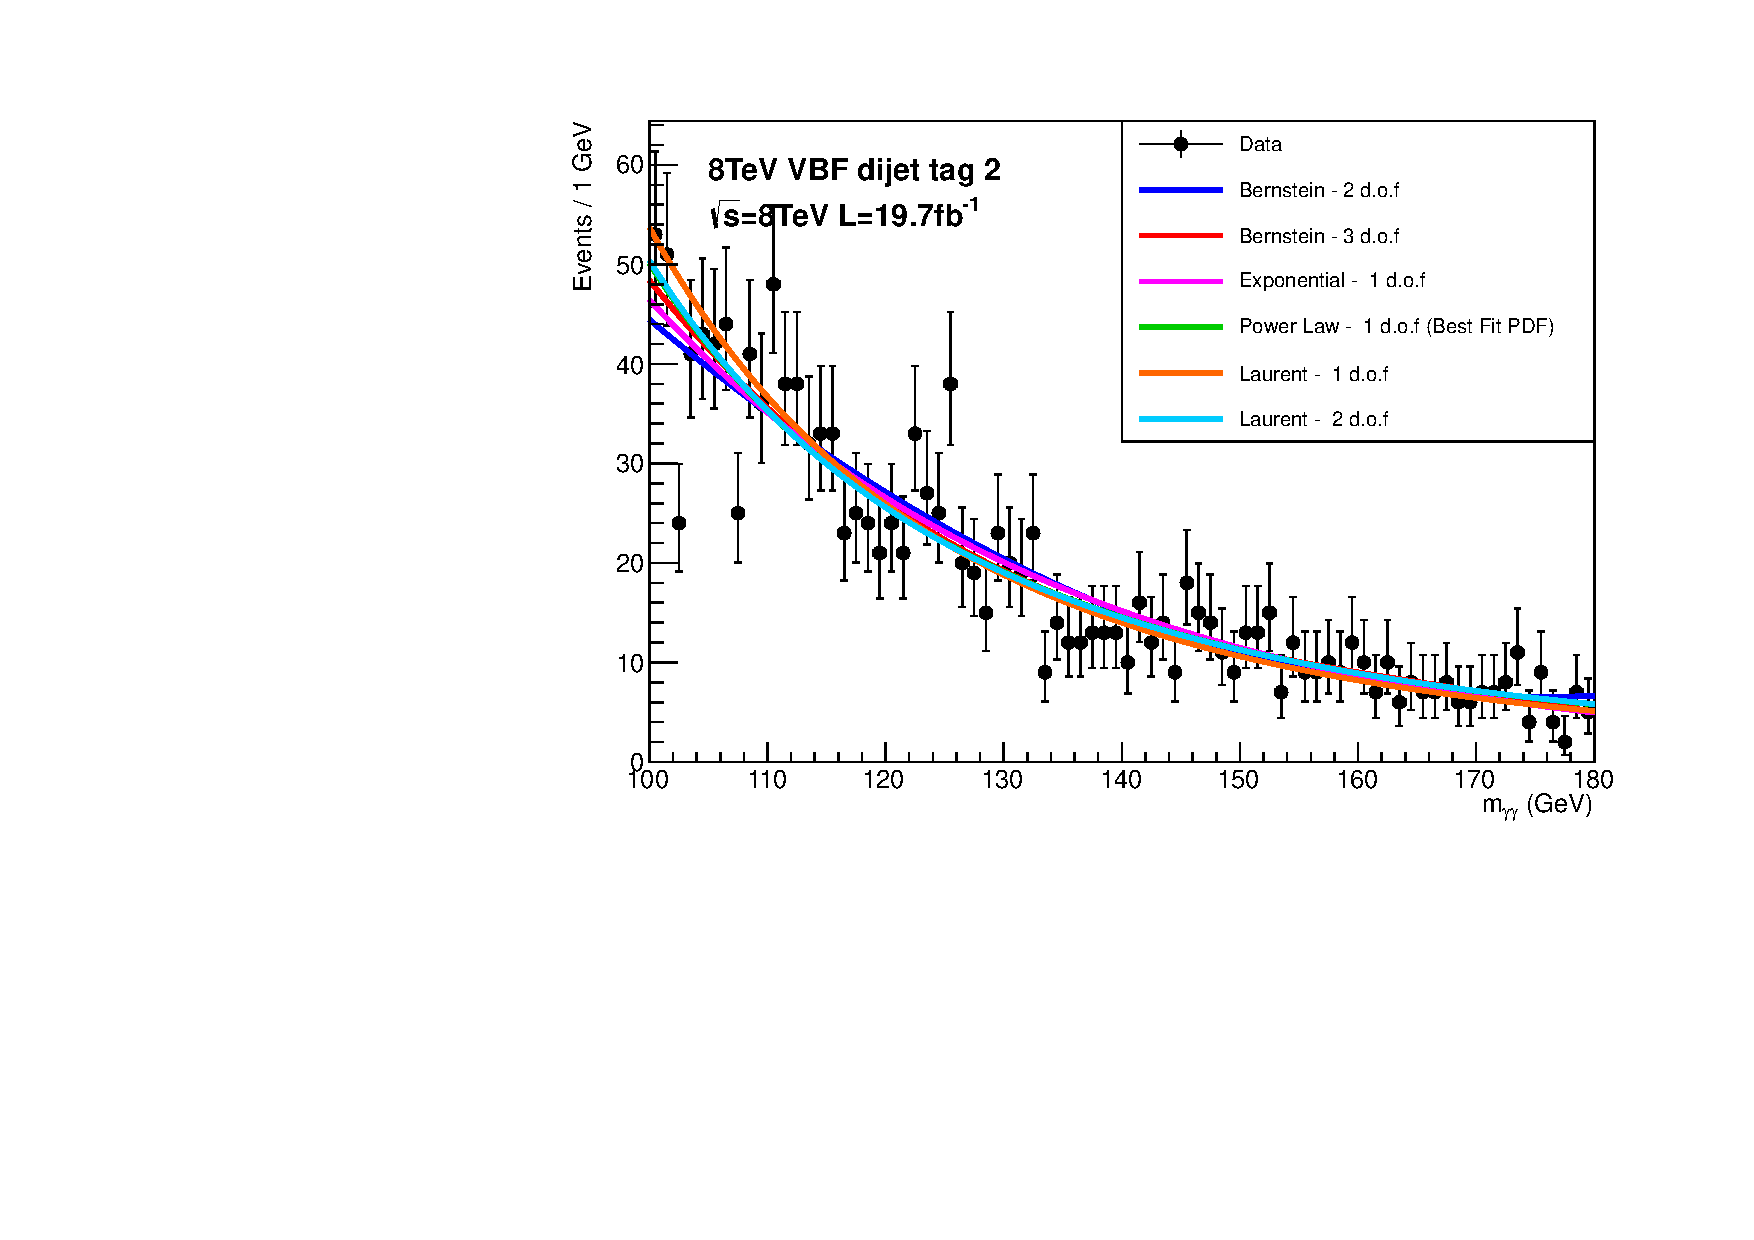
\includegraphics[width=0.49\textwidth]{analysis/plots/multipdf_plots/cat7_8TeV.pdf}
  \caption{The diphoton invariant mass distribution and the function choices for the background envelope for the dijet categories in the 8~\TeV dataset.}
  \label{fig:multipdf5}
\end{figure}

\begin{figure}
  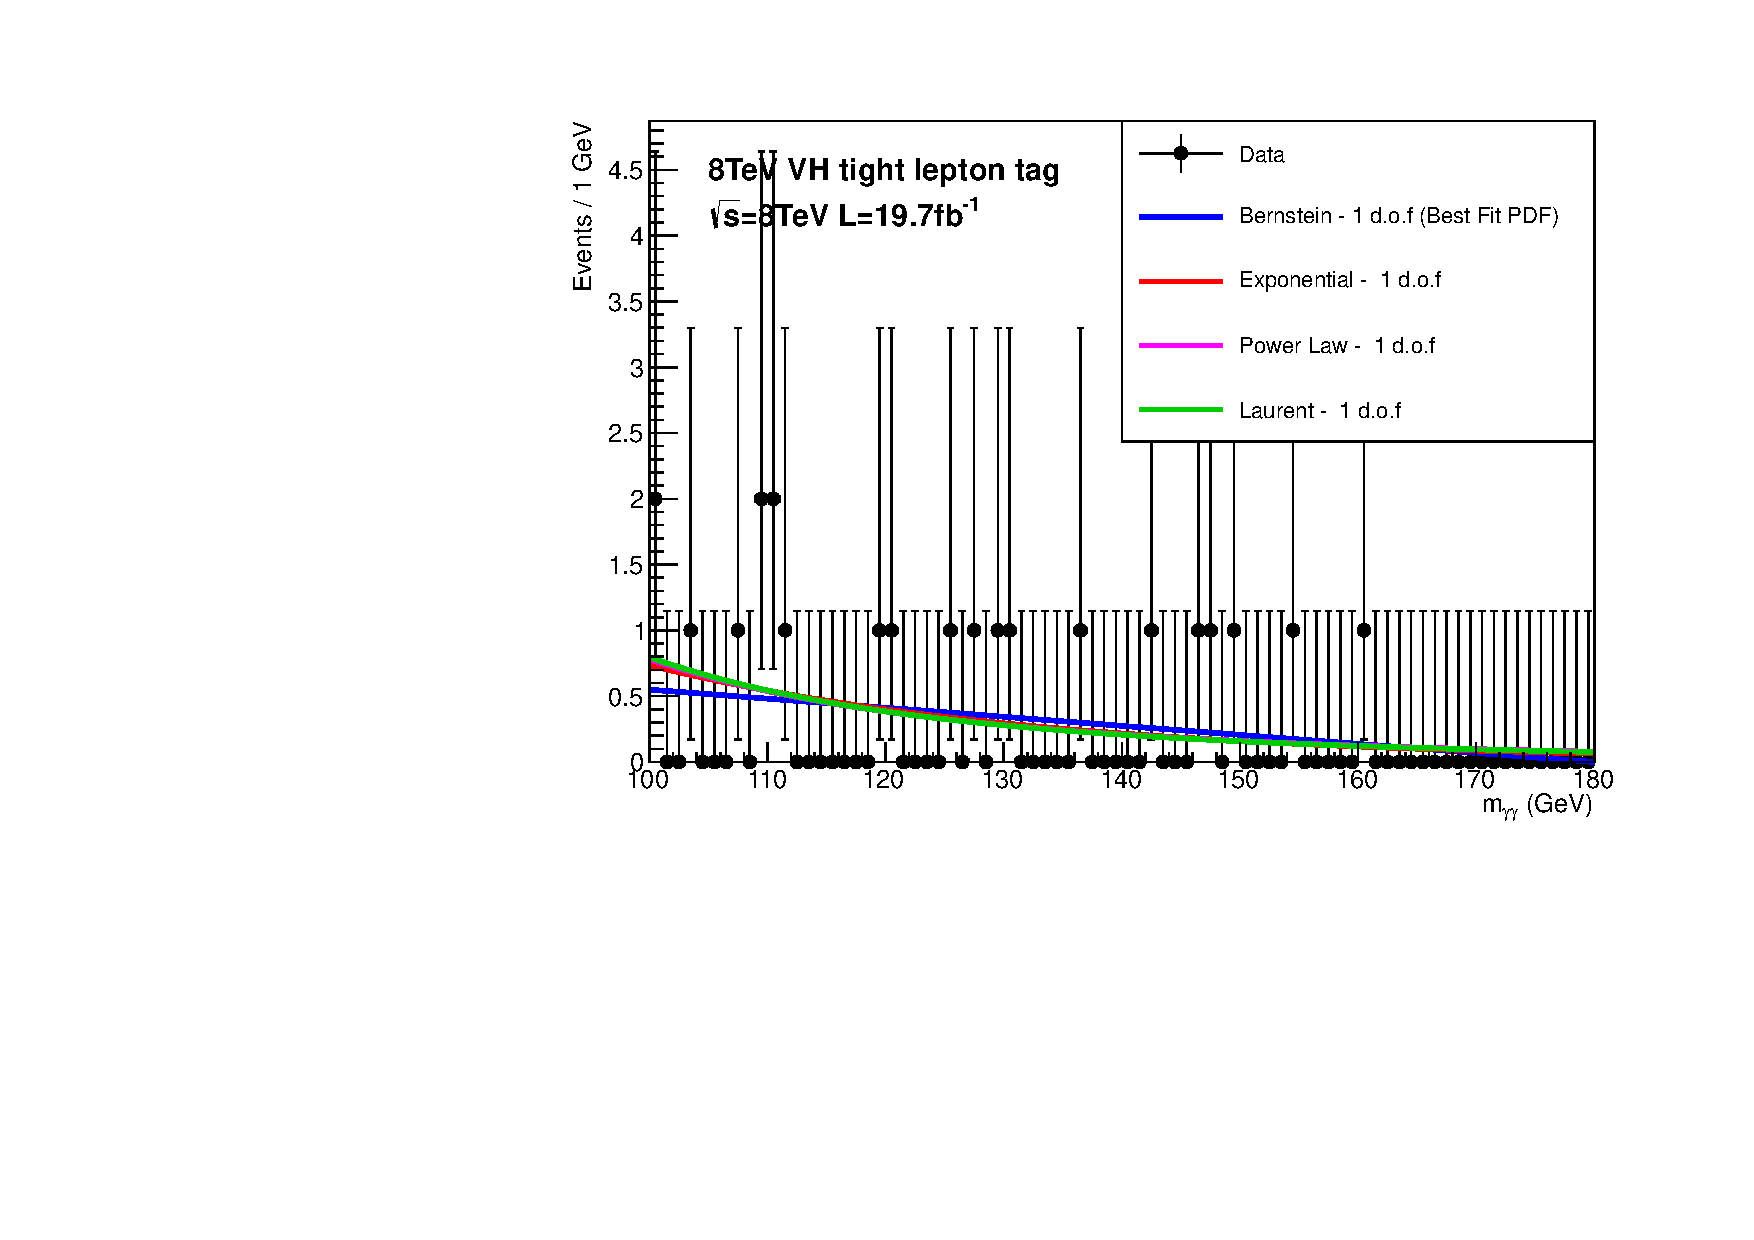
\includegraphics[width=0.49\textwidth]{analysis/plots/multipdf_plots/cat8_8TeV.pdf}
  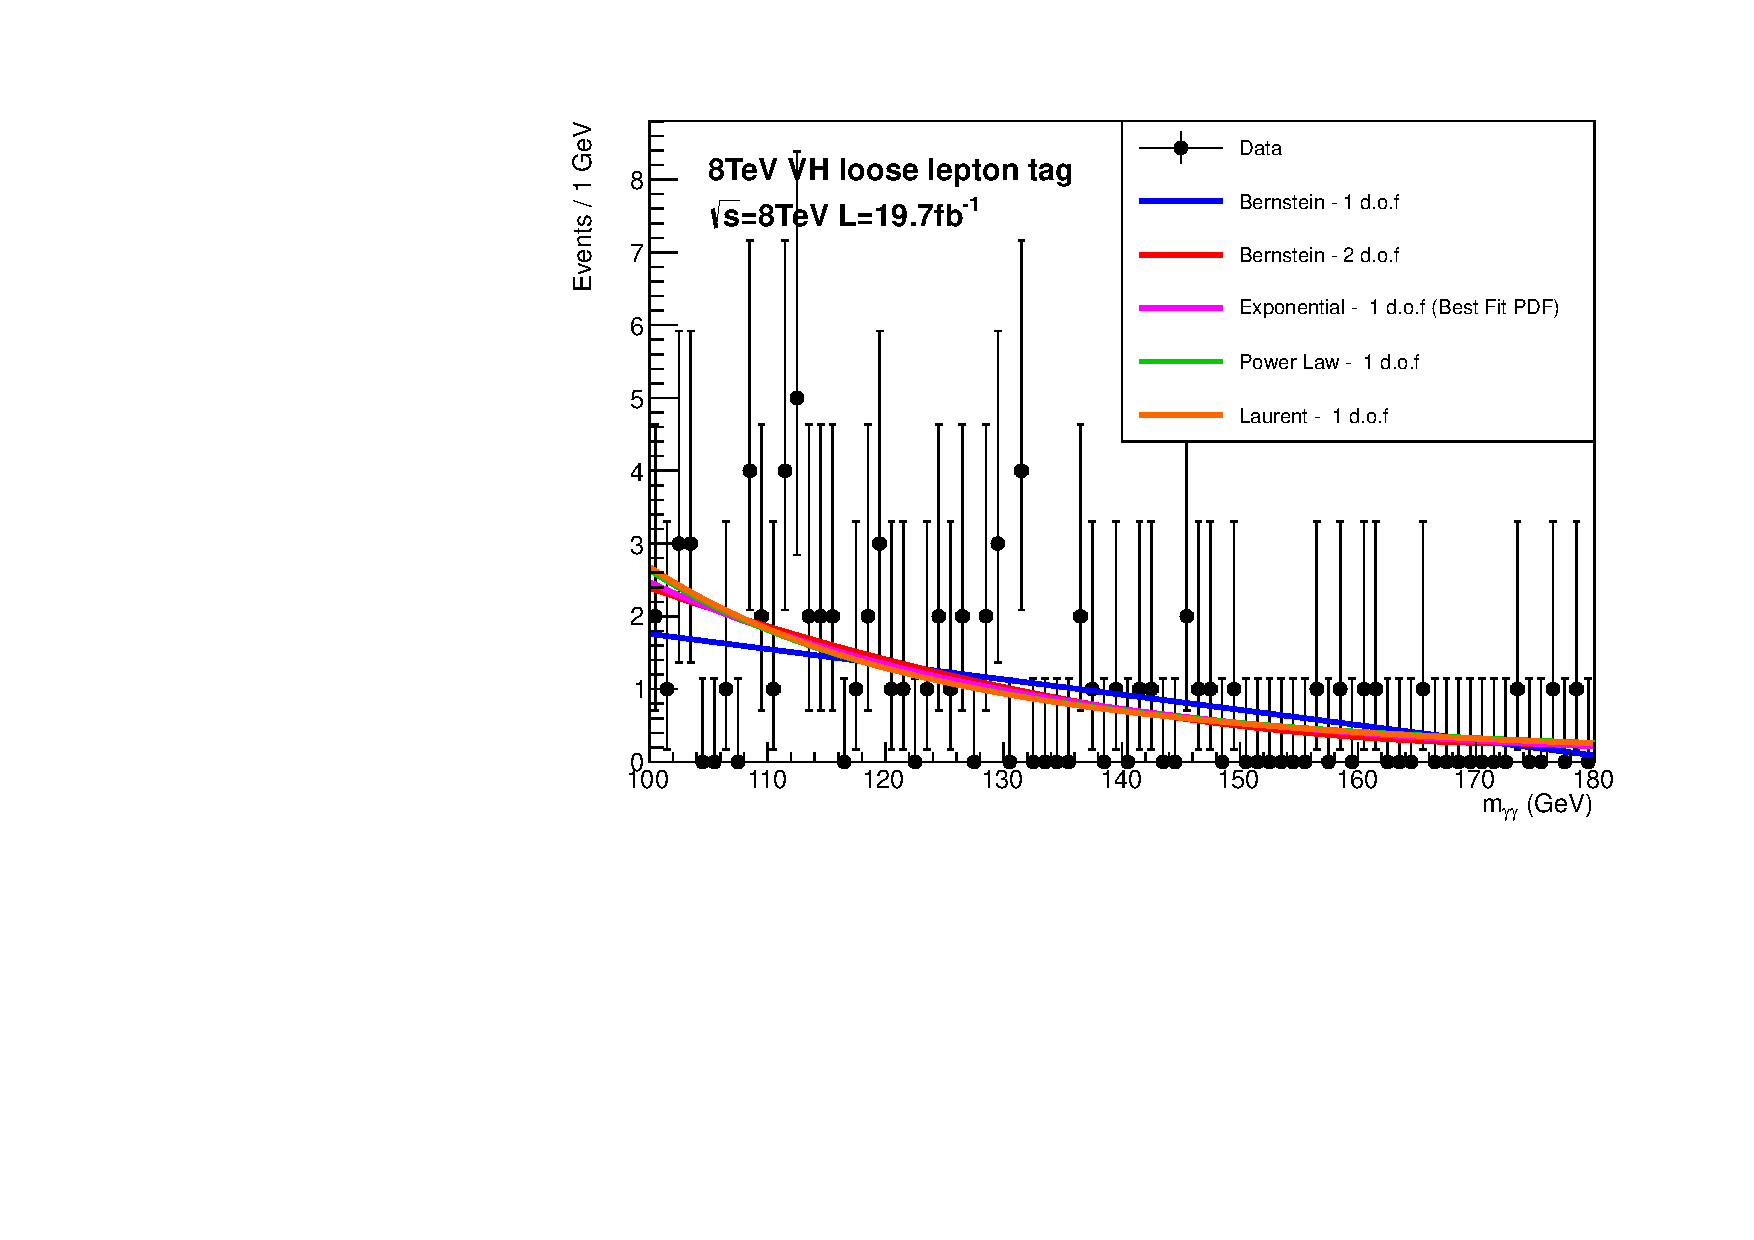
\includegraphics[width=0.49\textwidth]{analysis/plots/multipdf_plots/cat9_8TeV.pdf}\\
  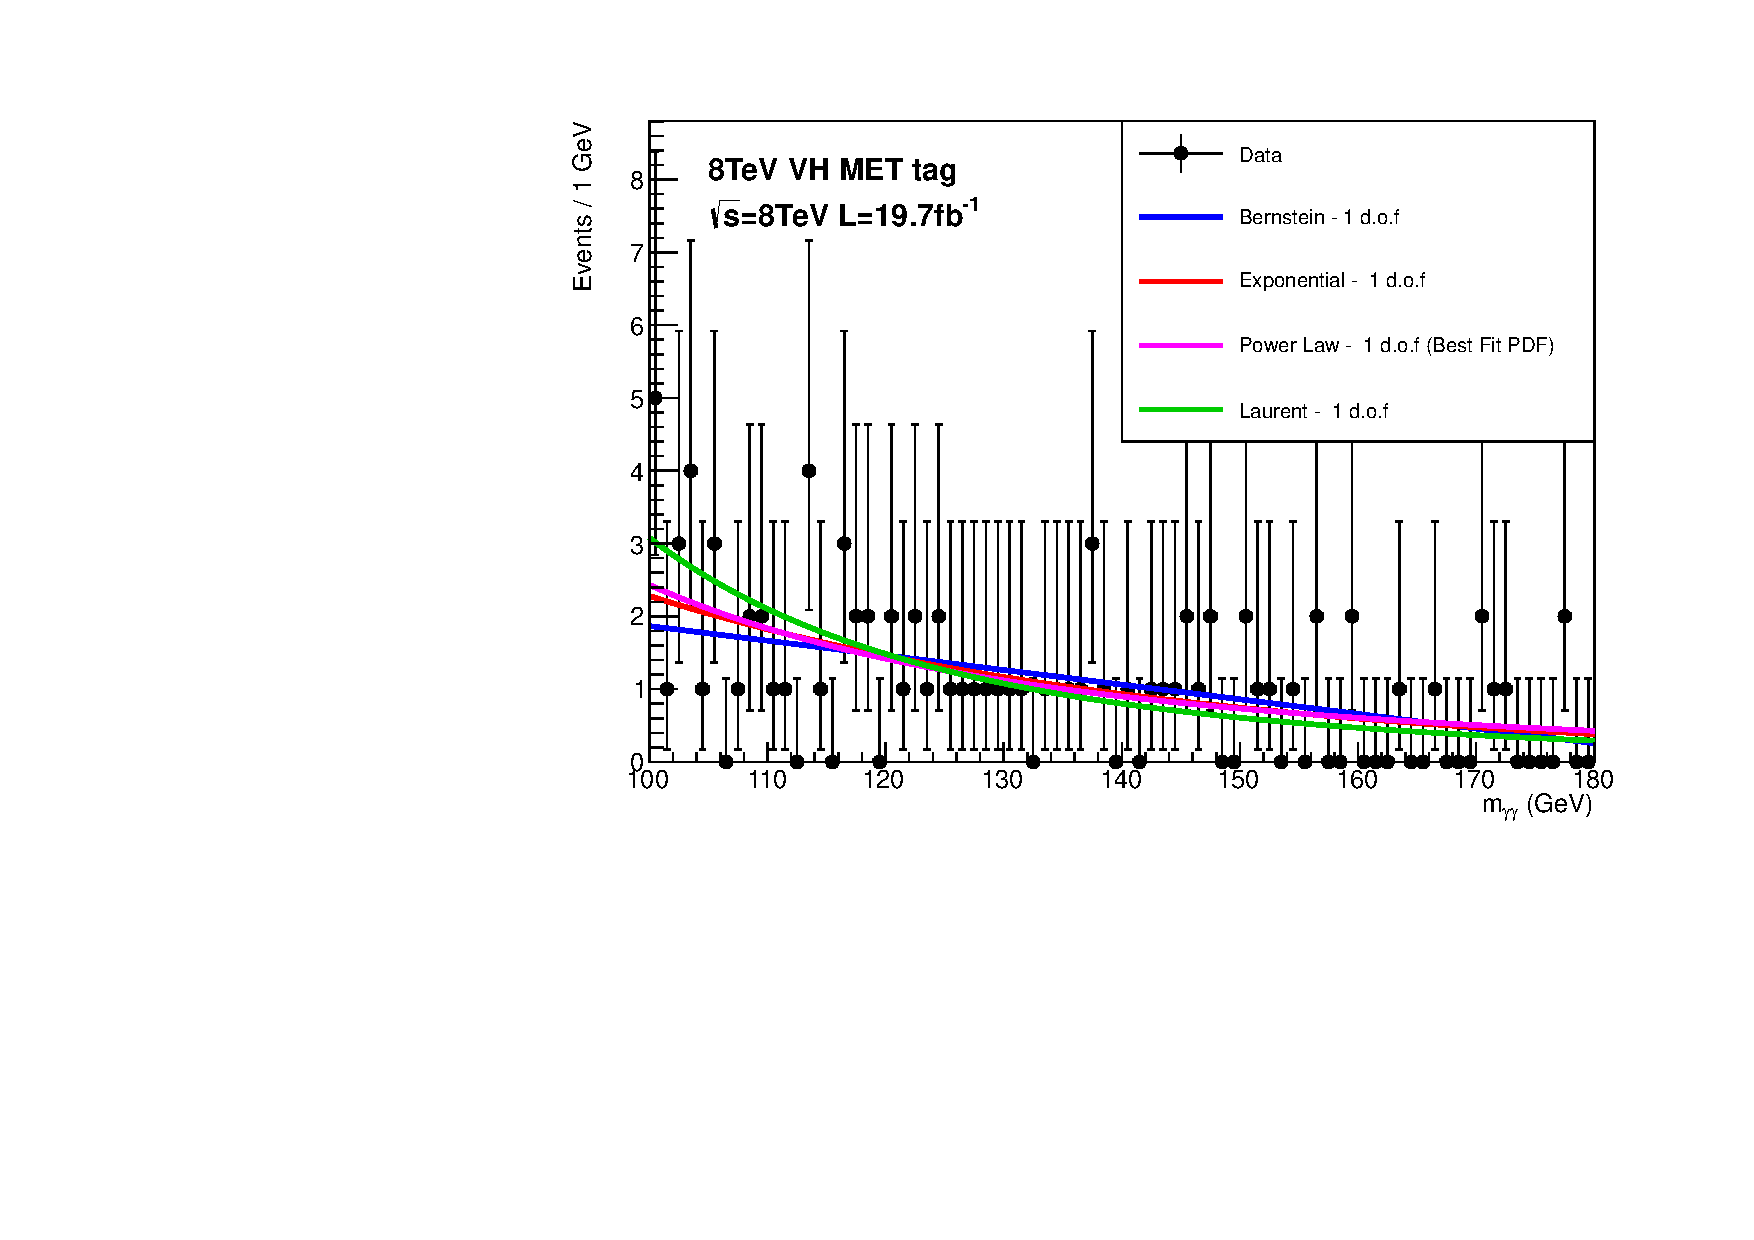
\includegraphics[width=0.49\textwidth]{analysis/plots/multipdf_plots/cat10_8TeV.pdf}
  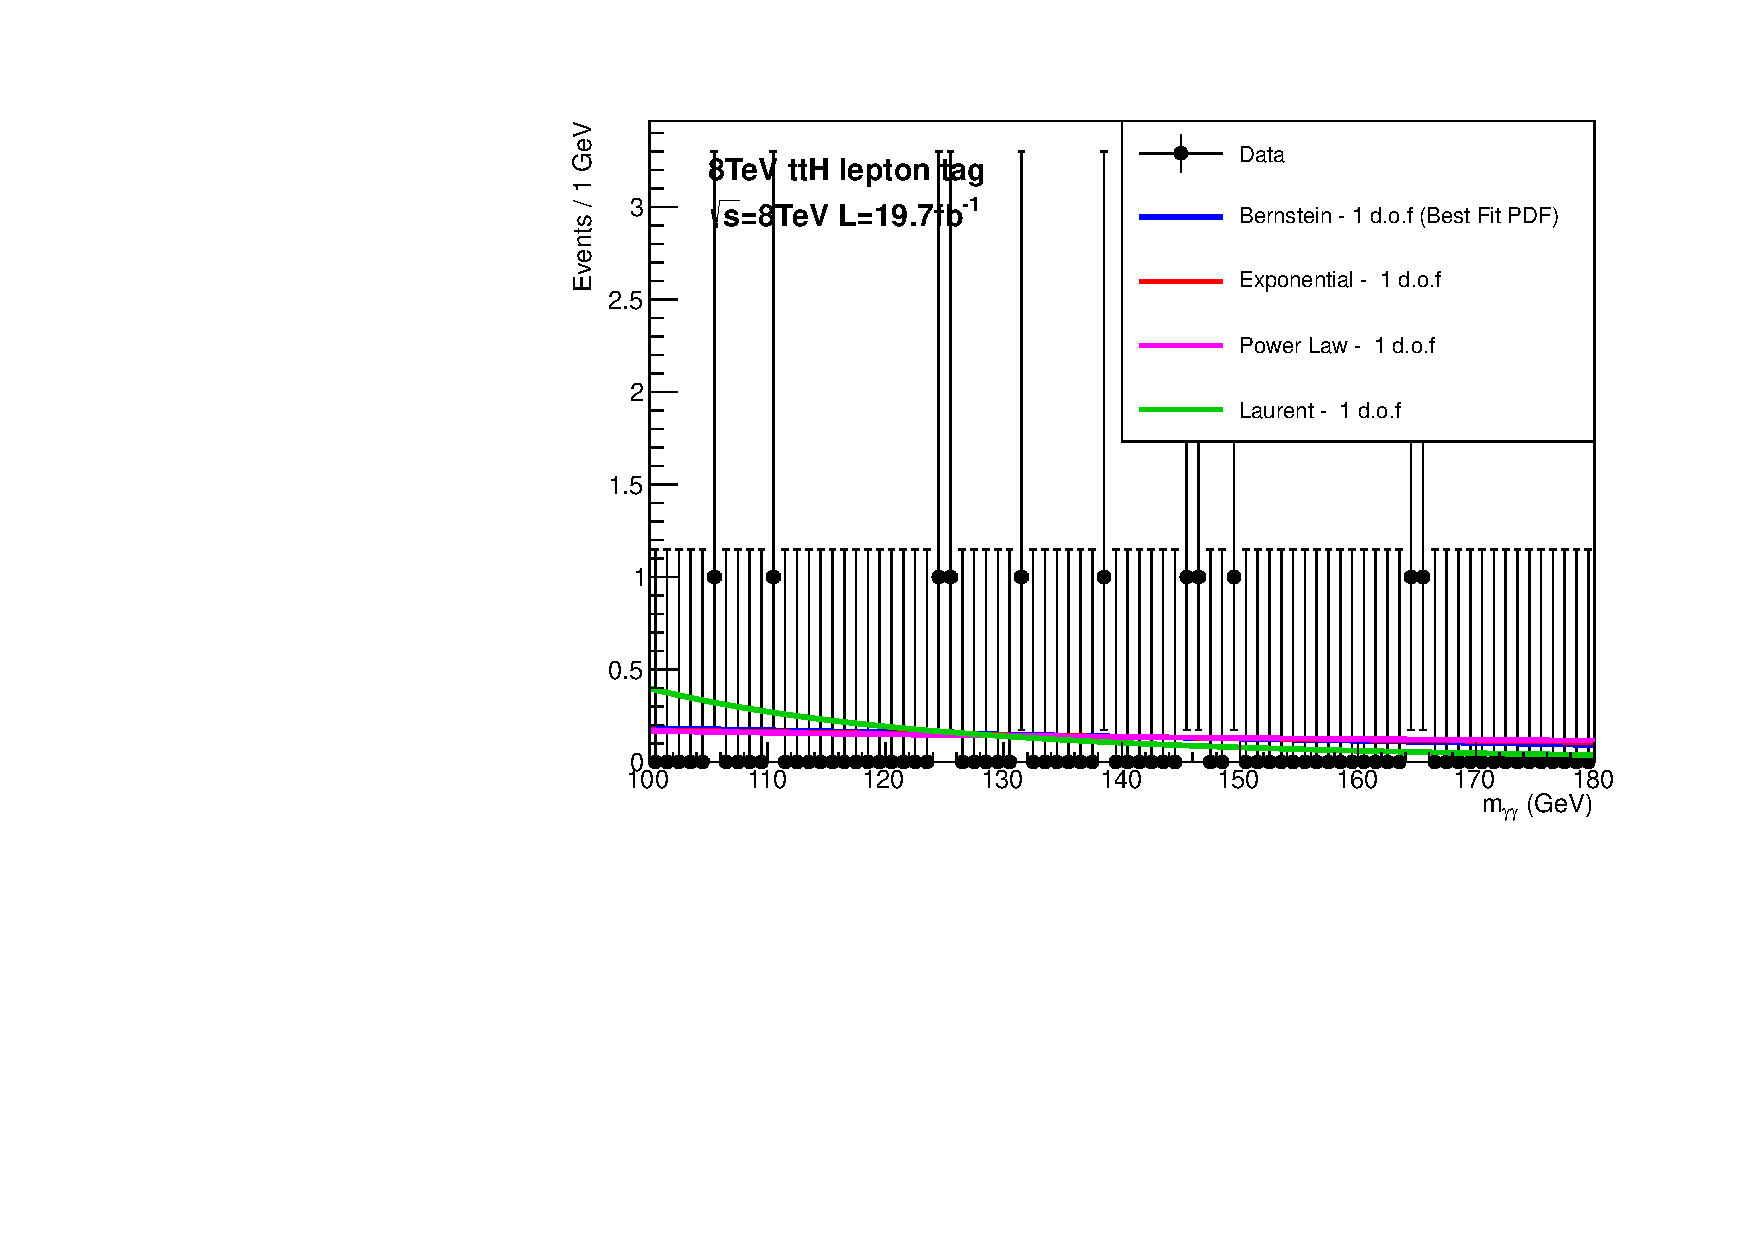
\includegraphics[width=0.49\textwidth]{analysis/plots/multipdf_plots/cat11_8TeV.pdf}\\
  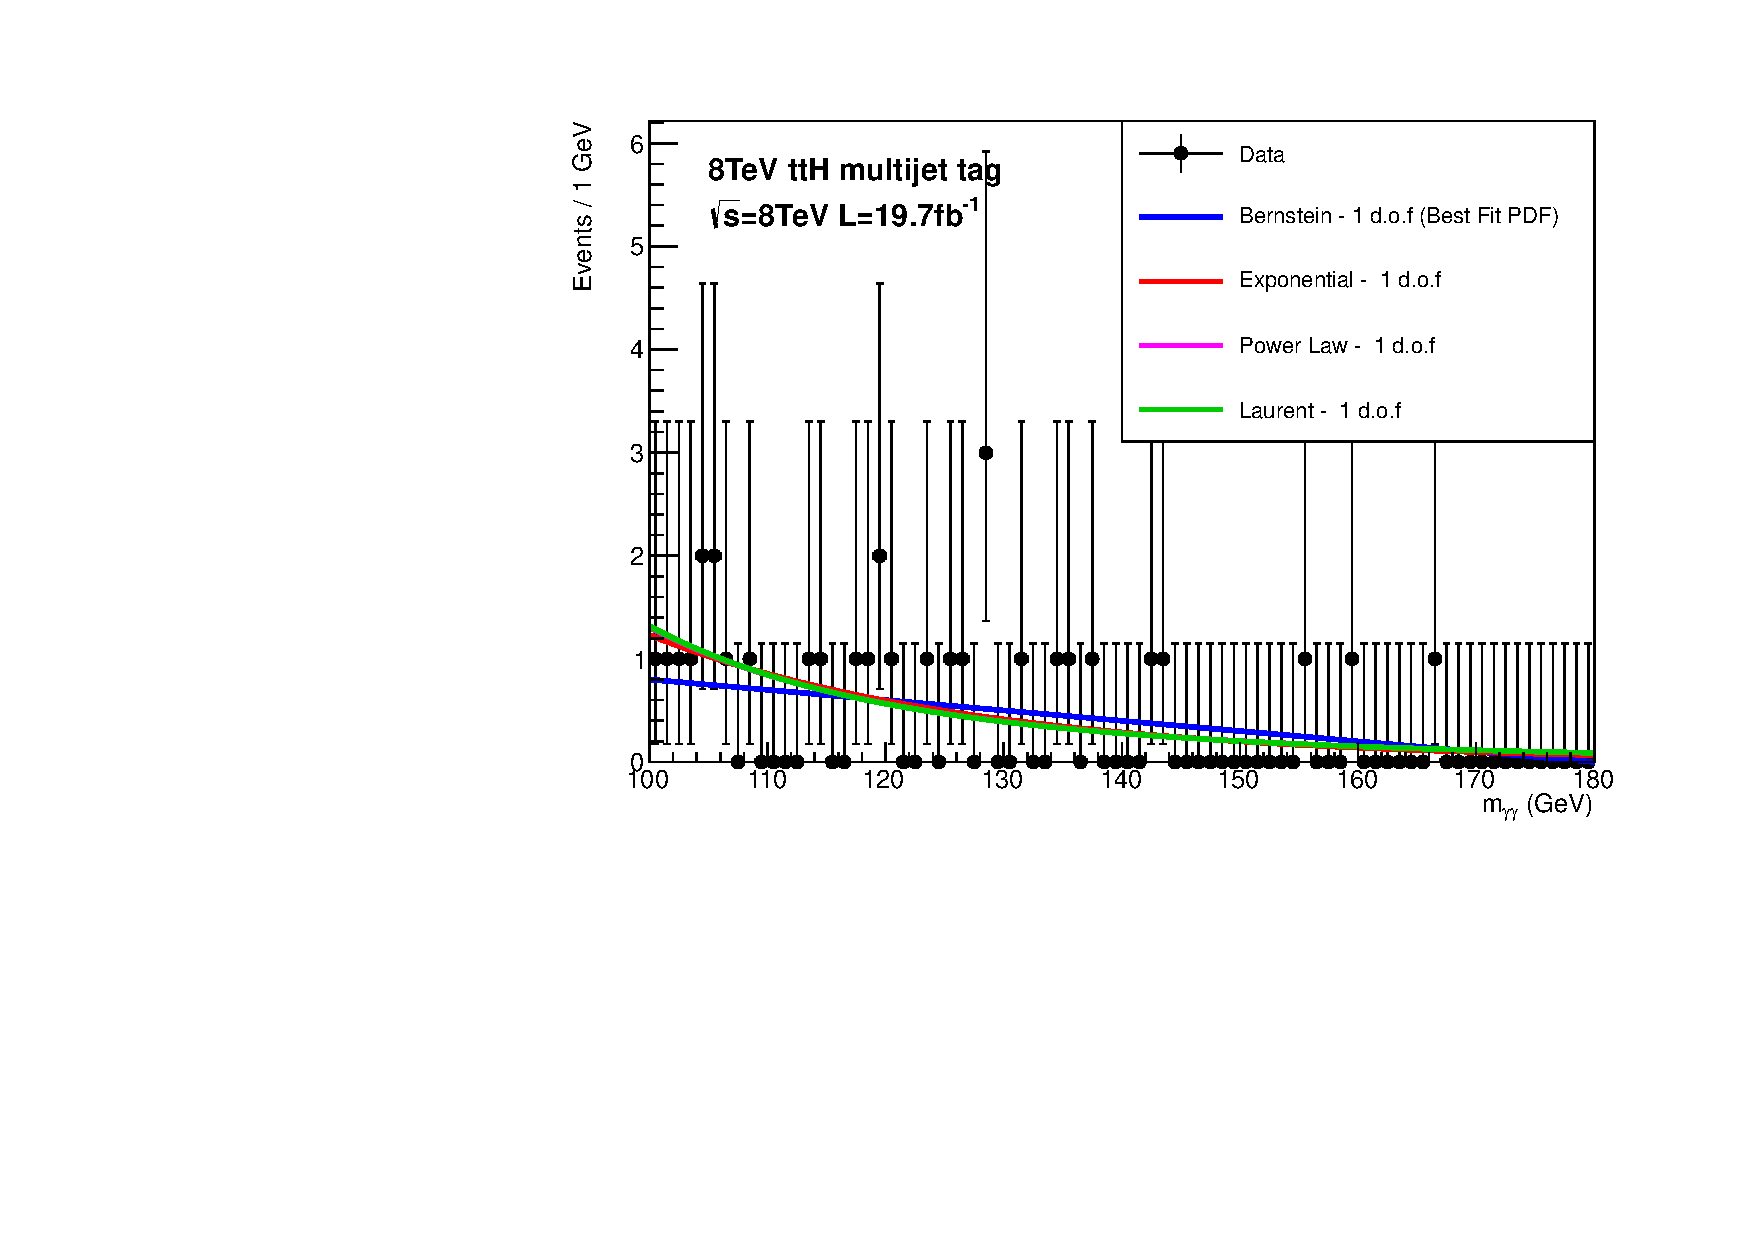
\includegraphics[width=0.49\textwidth]{analysis/plots/multipdf_plots/cat12_8TeV.pdf}
  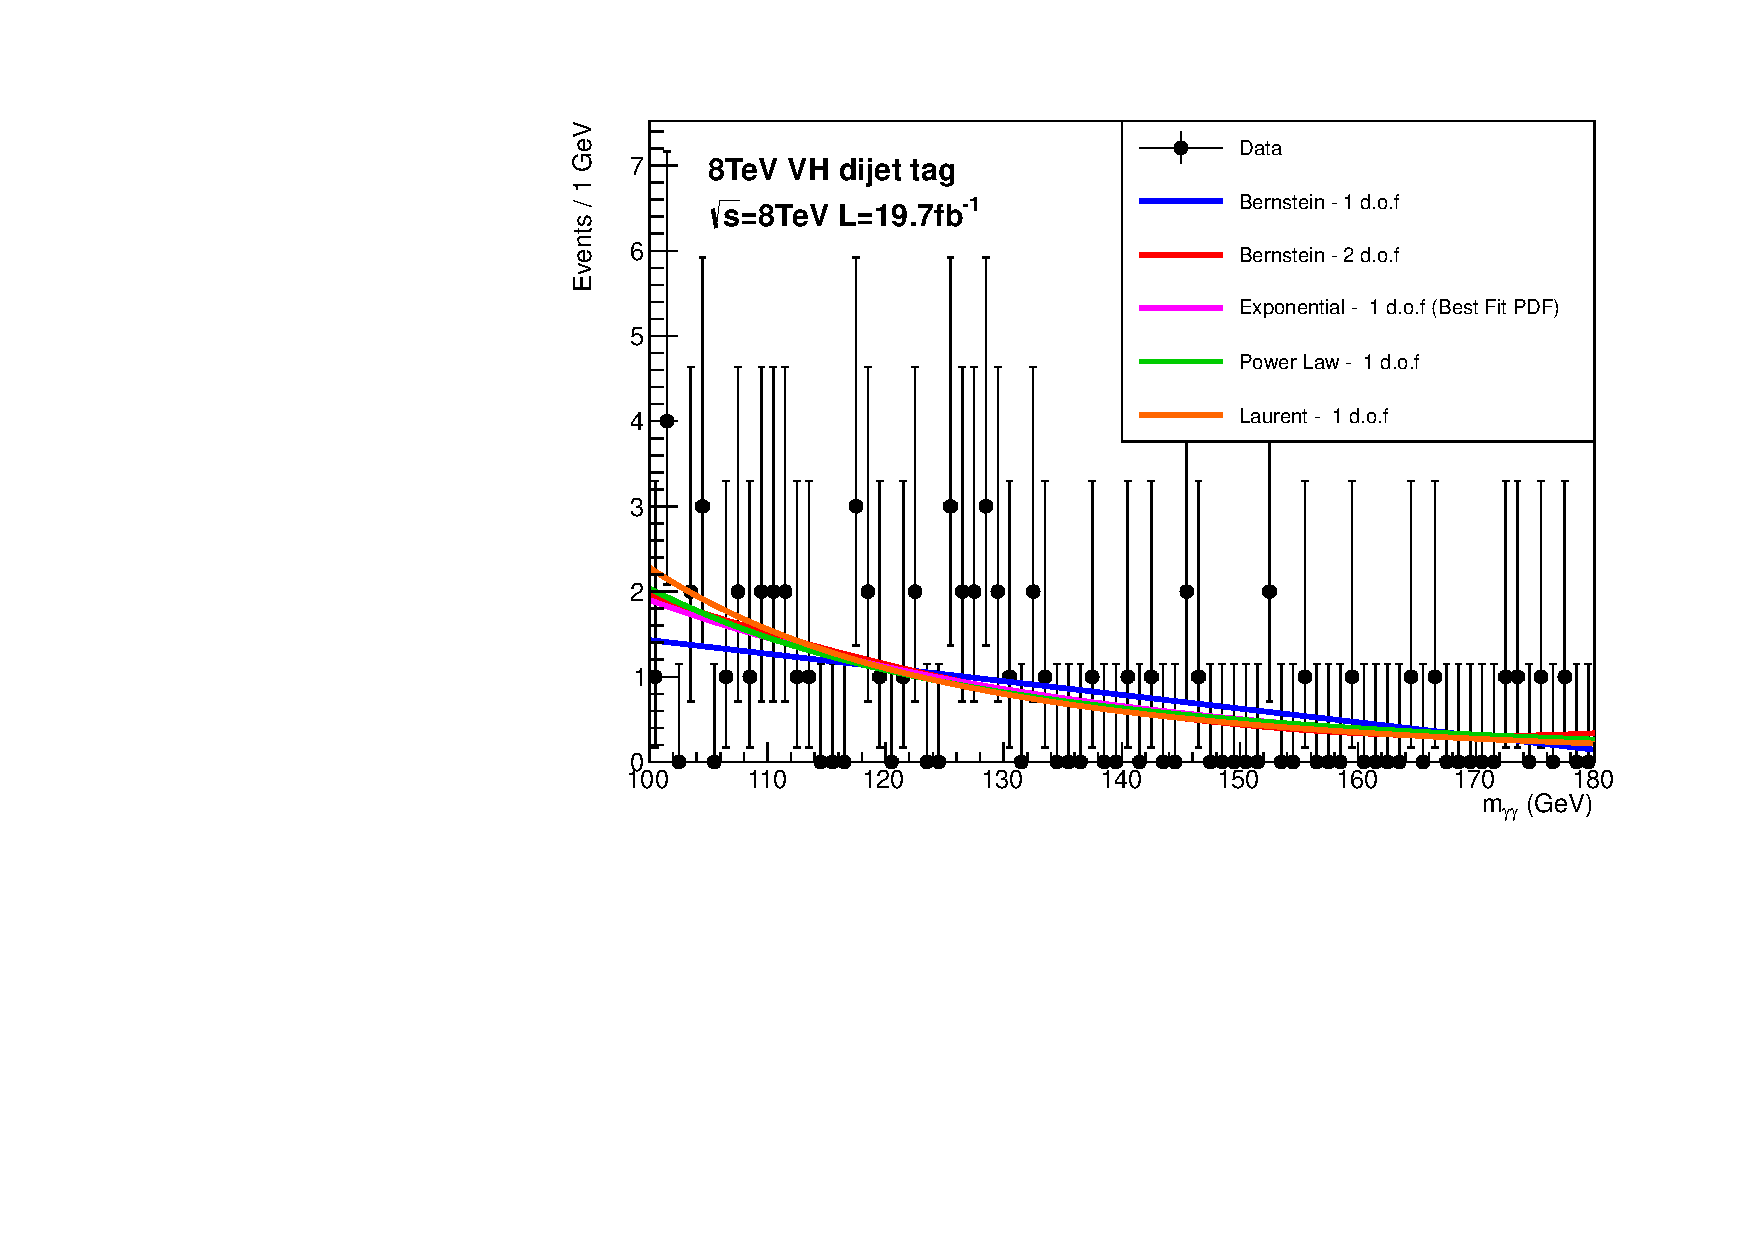
\includegraphics[width=0.49\textwidth]{analysis/plots/multipdf_plots/cat13_8TeV.pdf}\\
  \caption{The diphoton invariant mass distribution and the function choices for the background envelope for the \VH and \ttH categories in the 8~\TeV dataset.}
  \label{fig:multipdf6}
\end{figure}

\subsection{Sideband analysis}

In the sideband analysis the shape and normalisation of the background are obtained separately. The overall normalisation is extracted from a parametric fit of the entire invariant mass distribution excluding the $\pm$2\% signal window. The shape, which is to say the distribution of events in each analysis bin, is extracted from invariant mass sidebands. Each sideband is defined to have the equivalent width of $\pm$2\% relative to the invariant mass that corresponds to the centre of the sideband. For a \SM Higgs at 125~\GeV about 75\% of the signal is contained within the window. Consequently a sideband either side of the signal window is skipped and then three sidebands on either side of the hypothesised mass in question are used. Figure~\ref{fig:sideband_norm} shows the inclusive invariant mass distribution for the 8~\TeV dataset, the parametric function used to extract the normalisation of events in the window, the signal region (in red) and the six sidebands (in blue).

In order to avoid Drell-Yan contamination in the region of low invariant mass any sideband whose lower boundary is less than 100~\GeV is removed and an additional sideband is added to the high side of the signal region. Consequently any mass hypothesis in the range $111\leq\mH< 115.5$~GeV has two lower and four upper sidebands and any mass hypothesis in the range $100\leq\mH<111$~GeV has one lower and five upper sidebands.

\begin{figure}
  \begin{center}
    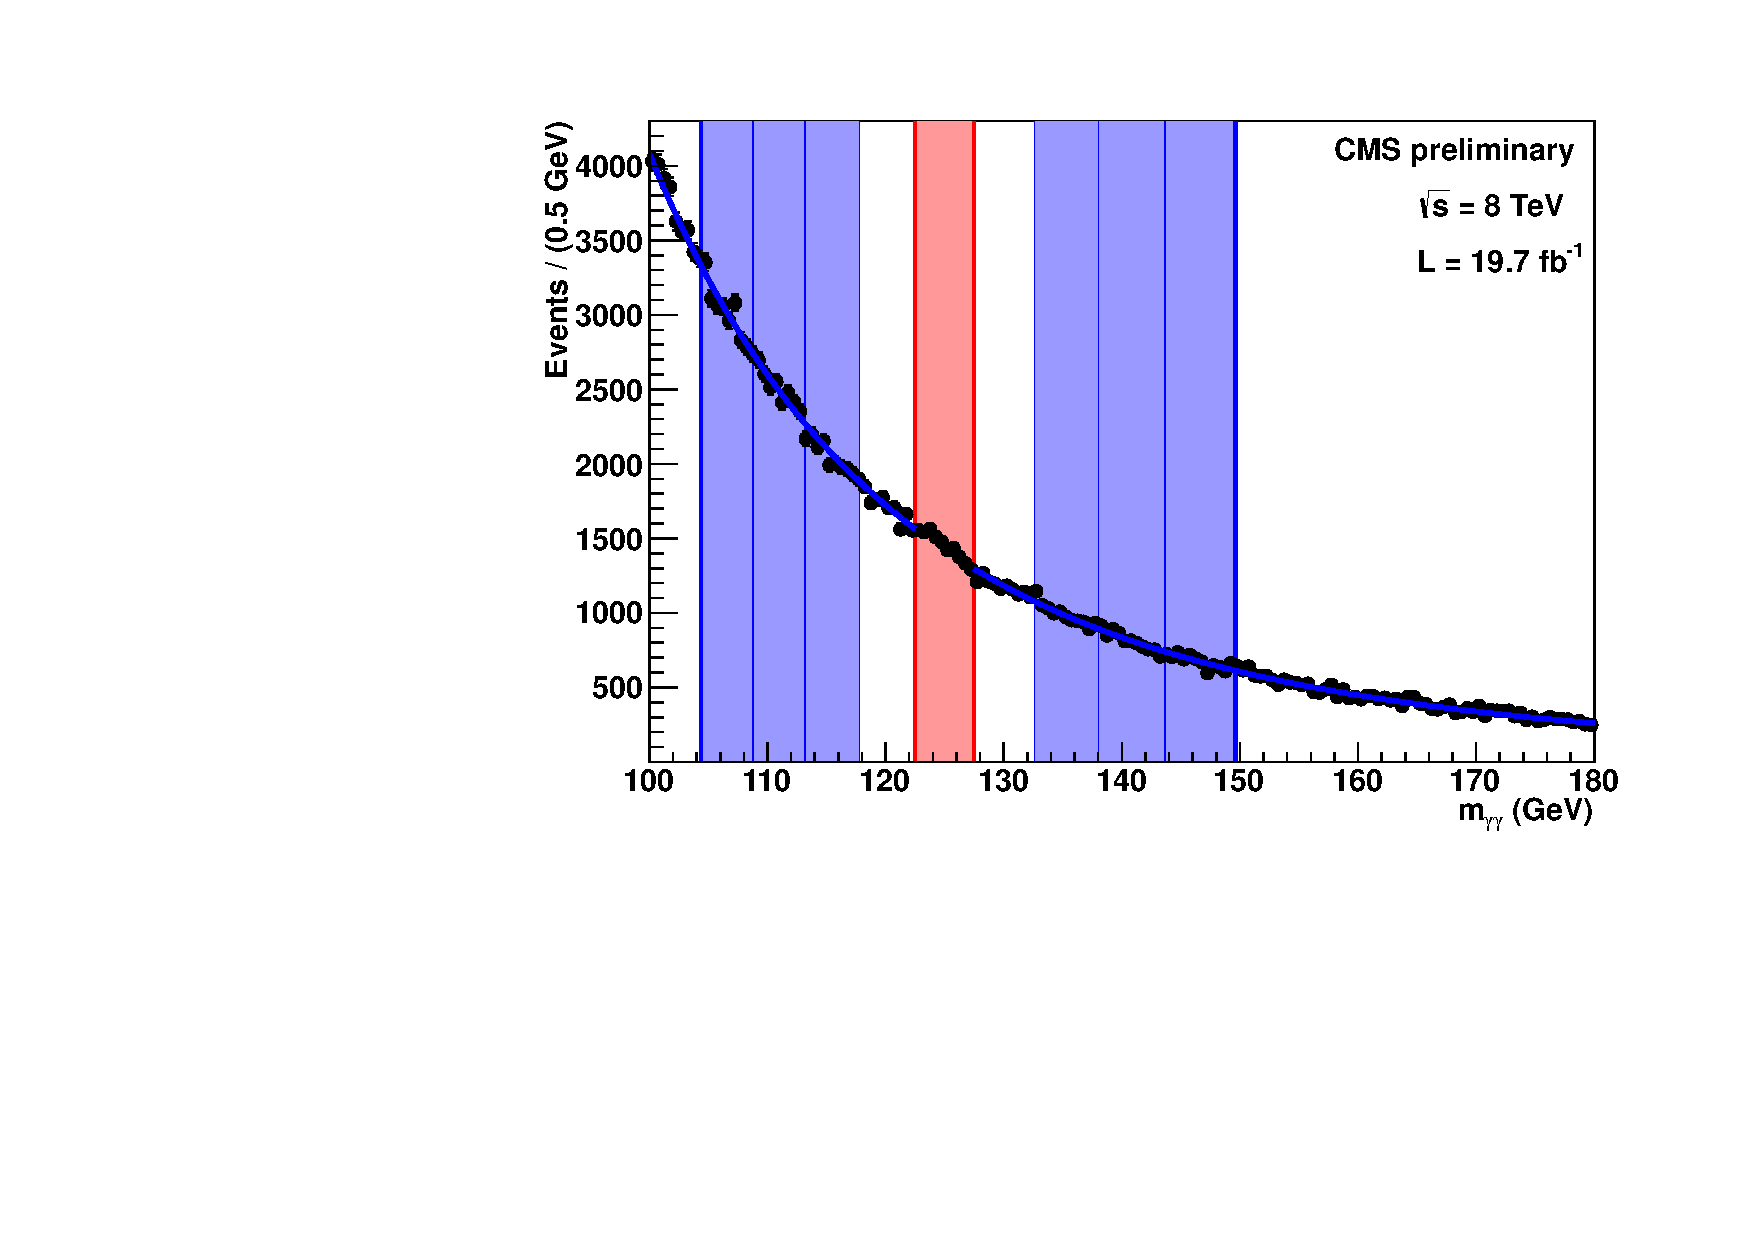
\includegraphics[width=0.85\textwidth]{analysis/plots/sideband/invmass.pdf}
    \caption[The invariant mass distribution for the 8~\TeV dataset]{The inclusive invariant mass distribution for the 8TeV dataset in data (black points). An illustration of the signal region (red) and the sidebands (blue) used for the mass hypothesis \mH=125~\GeV is shown. The parametric function used to obtain the normalisation in the signal region is shown as the blue line.}
    \label{fig:sideband_norm}
  \end{center}
\end{figure}

The parametric form used to obtain the normalisation is a single term power law (one degree of freedom) for the 8~\TeV dataset and a two term Laurent series (one degree of freedom) for the 7~\TeV dataset. The functions are defined identically to those described for the envelope method in Sec.~\ref{sec:envelope}. These functions are chosen because they give the smallest uncertainty when accounting for biases incurred by picking the wrong functional form. A systematic uncertainty is applied to the normalisation term of which there are more details in Sec.~\ref{sec:systematics}.

The estimated number of background events in the signal region is obtained from the data in the sidebands. It is assumed that the fraction of events in each bin varies linearly with invariant mass (i.e.~across sidebands) and that there is negligible signal contamination in the sidebands. For each bin, $b$, the fraction of events for a given mass is taken to be,
\begin{equation}
  f_{b} = p_{0b} + p_{1b}(m-m_{H}),
\end{equation}
where $p_{0b}$ and $p_{1b}$ are the Taylor expansion coefficients for bin $b$. Since the fractions must sum to unity for any given mass (the normalisation is extracted elsewhere) then for $N$ bins there are $2(N-1)$ coefficiets. These coefficients are determined by fitting a straight line across the sidebands in each bin, with the constraint that the fraction in each sideband must sum to 1 across all the bins. An example of ones of these fits is shown in Fig.~\ref{fig:sideband_shape}.

\begin{figure}
  \begin{center}
    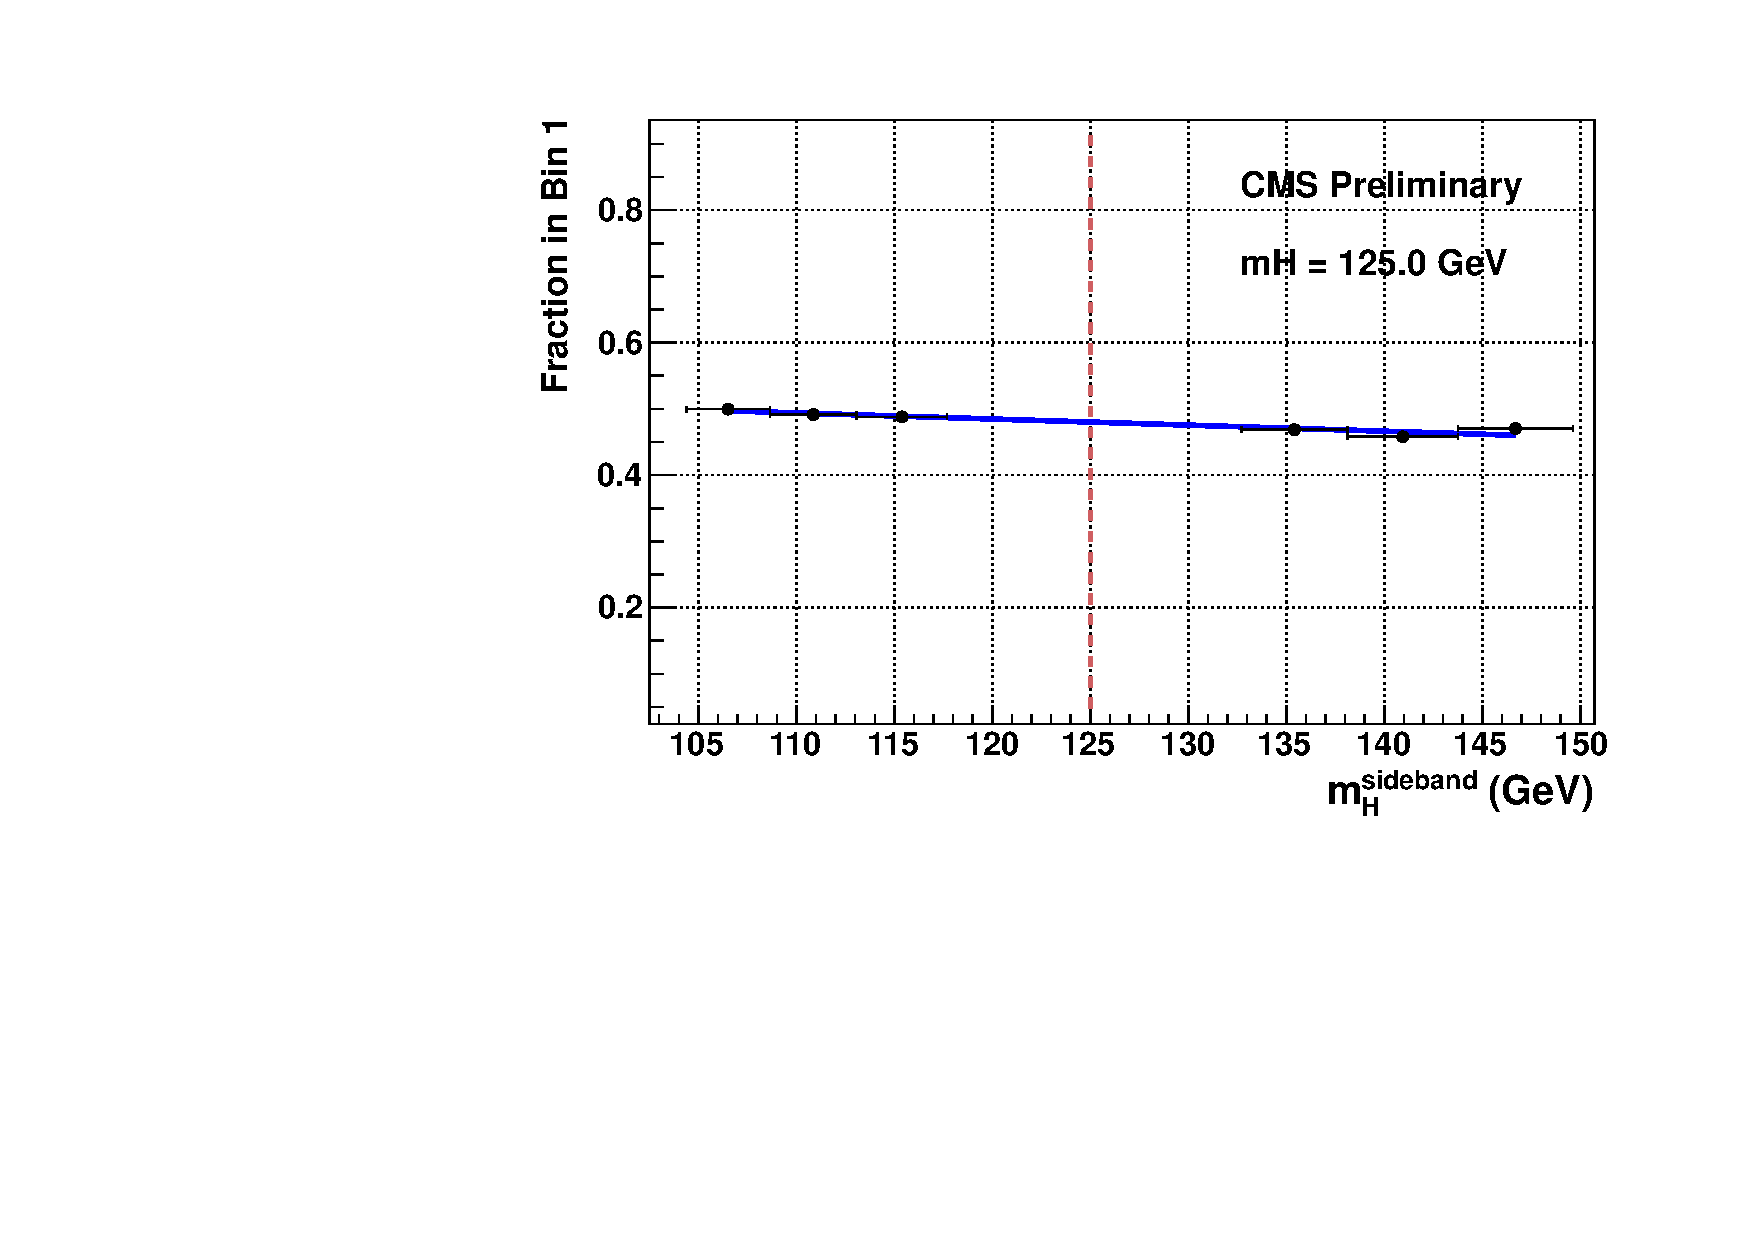
\includegraphics[width=0.85\textwidth]{analysis/plots/sideband/sideband_fit.pdf}
    \caption[An example of one of the sideband fits for the \SMVA]{The fraction of data events in a single analysis bin in each of the sidebands surrounding the signal window at \mH=125~\GeV (black points). The blue line show the straight line fit for this bin. In the 8~\TeV dataset there are 10 inclusive analysis bins and 9 exclusive analysis bins. Consequently there are 19 of these straight line fits at each \mH but only 18 of them are independent as the fractions must sum to unity.}
    \label{fig:sideband_shape}
  \end{center}
\end{figure}

The distribution for the data, background (along with the $\pm1\sigma$ and $\pm2\sigma$ errors) and signal for each of the sideband analysis bins are shown in Fig.~\ref{fig:sideband_output} for the mass hypothesis, \mH=124.7~\GeV.

\begin{figure}
  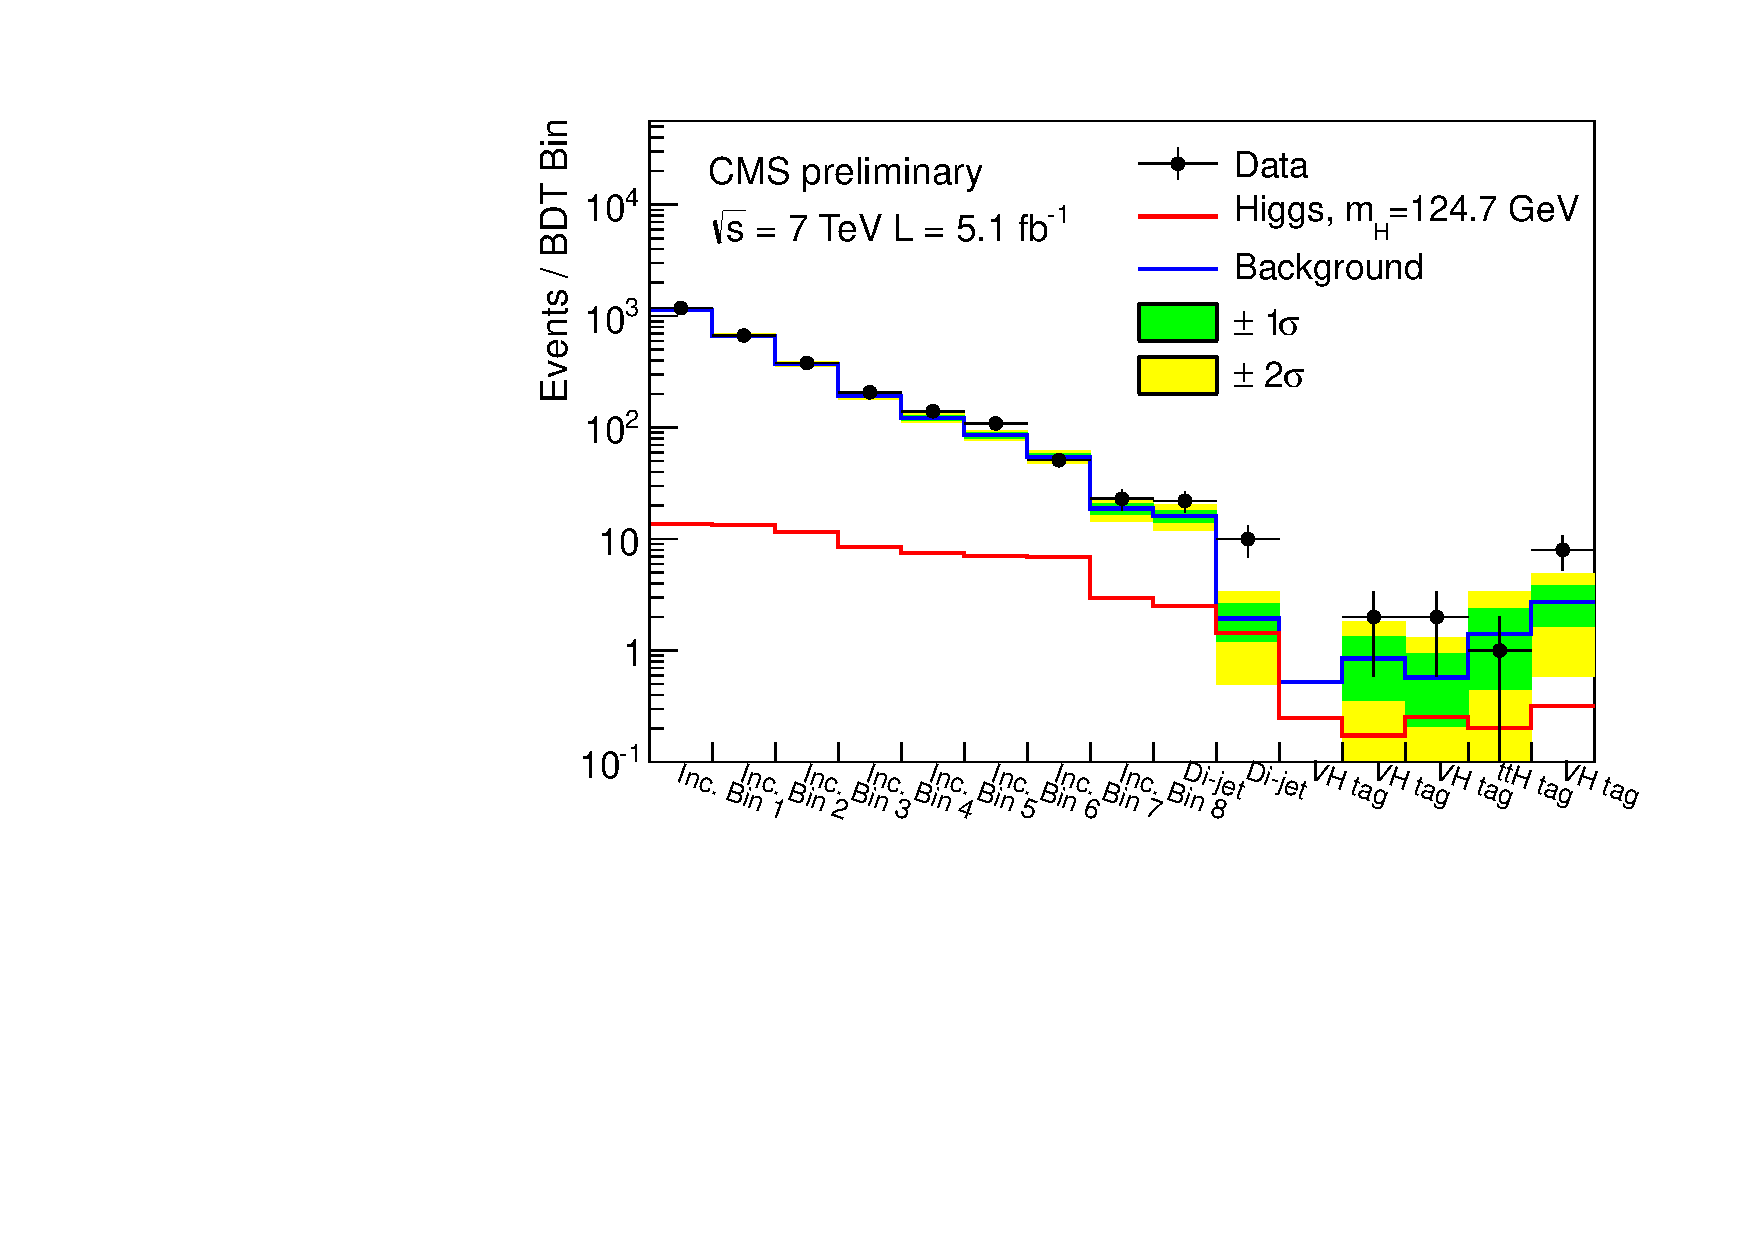
\includegraphics[width=0.48\textwidth]{{analysis/plots/sideband/model_7TeV_m124.7}.pdf}
  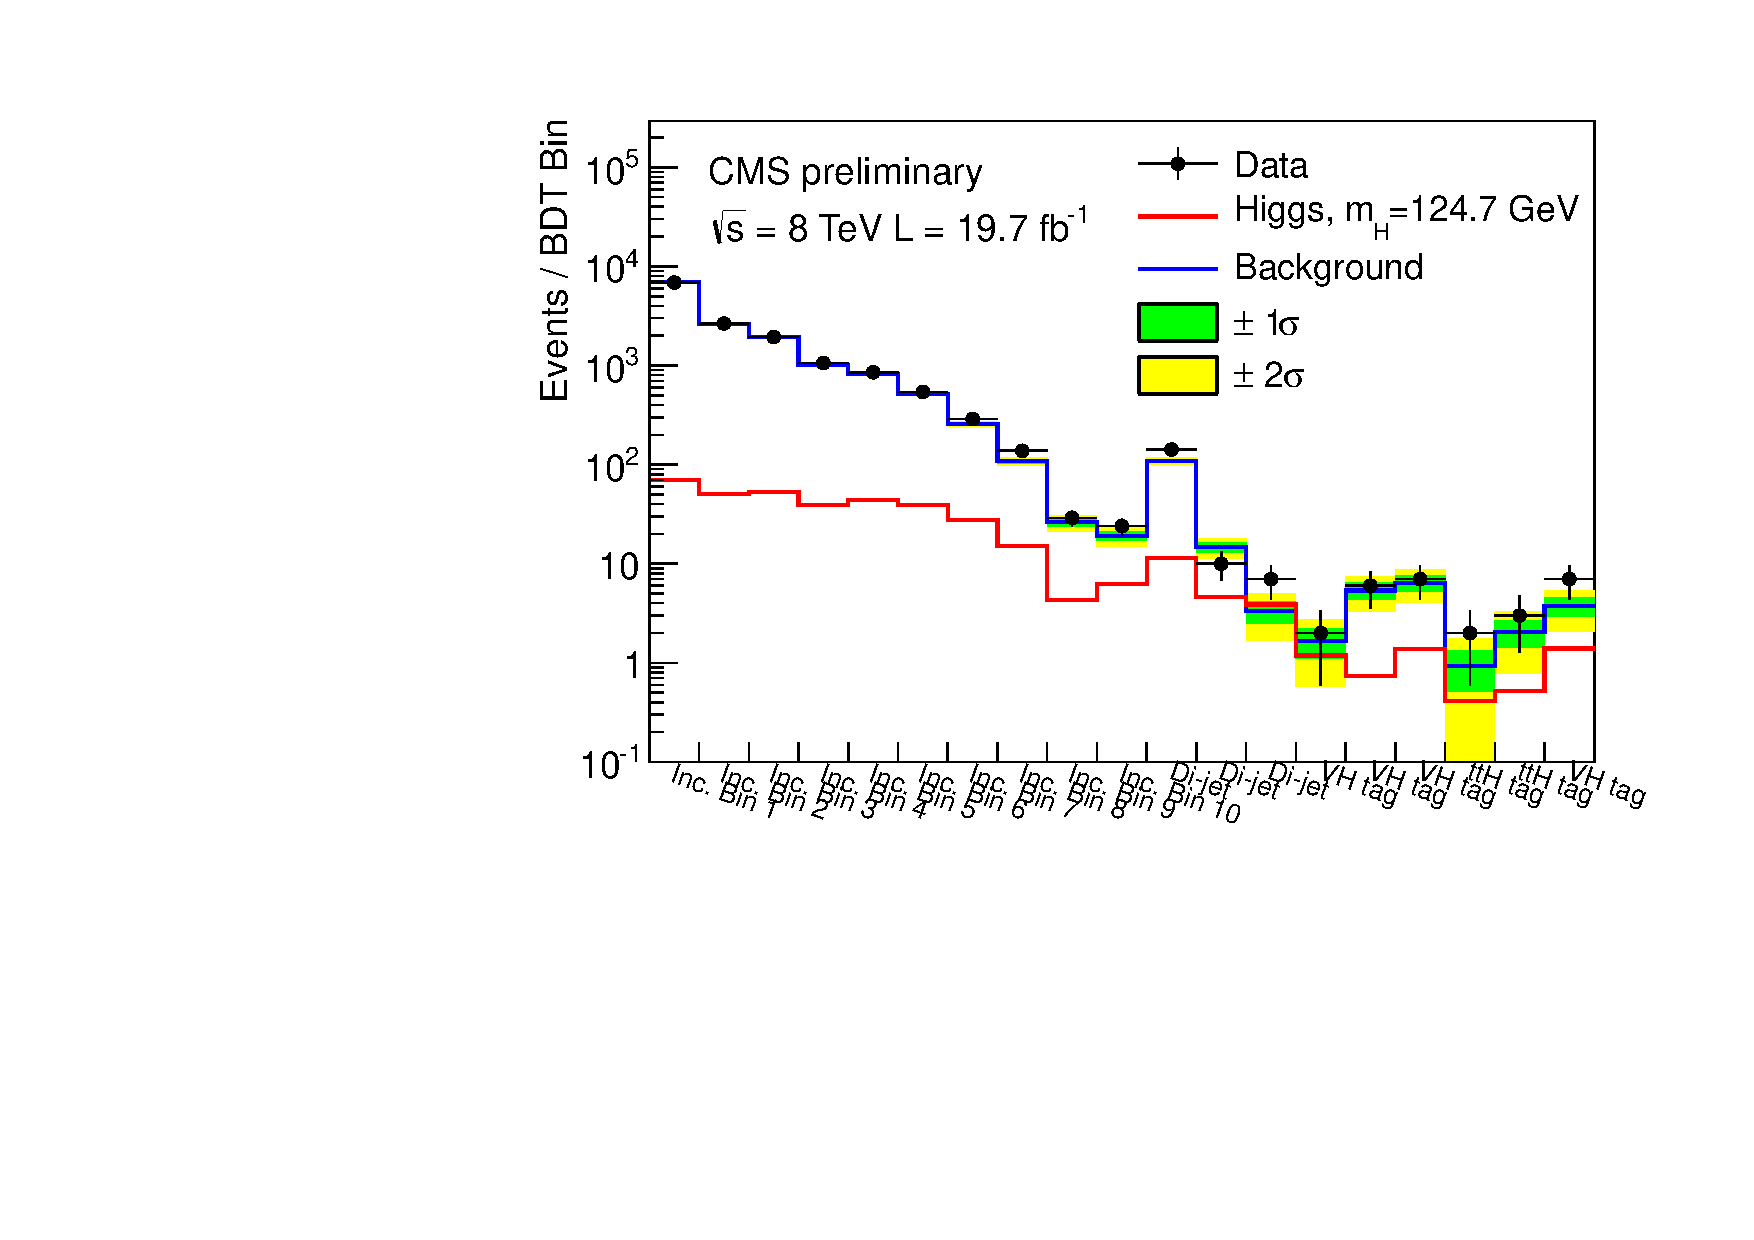
\includegraphics[width=0.48\textwidth]{{analysis/plots/sideband/model_8TeV_m124.7}.pdf}\\
  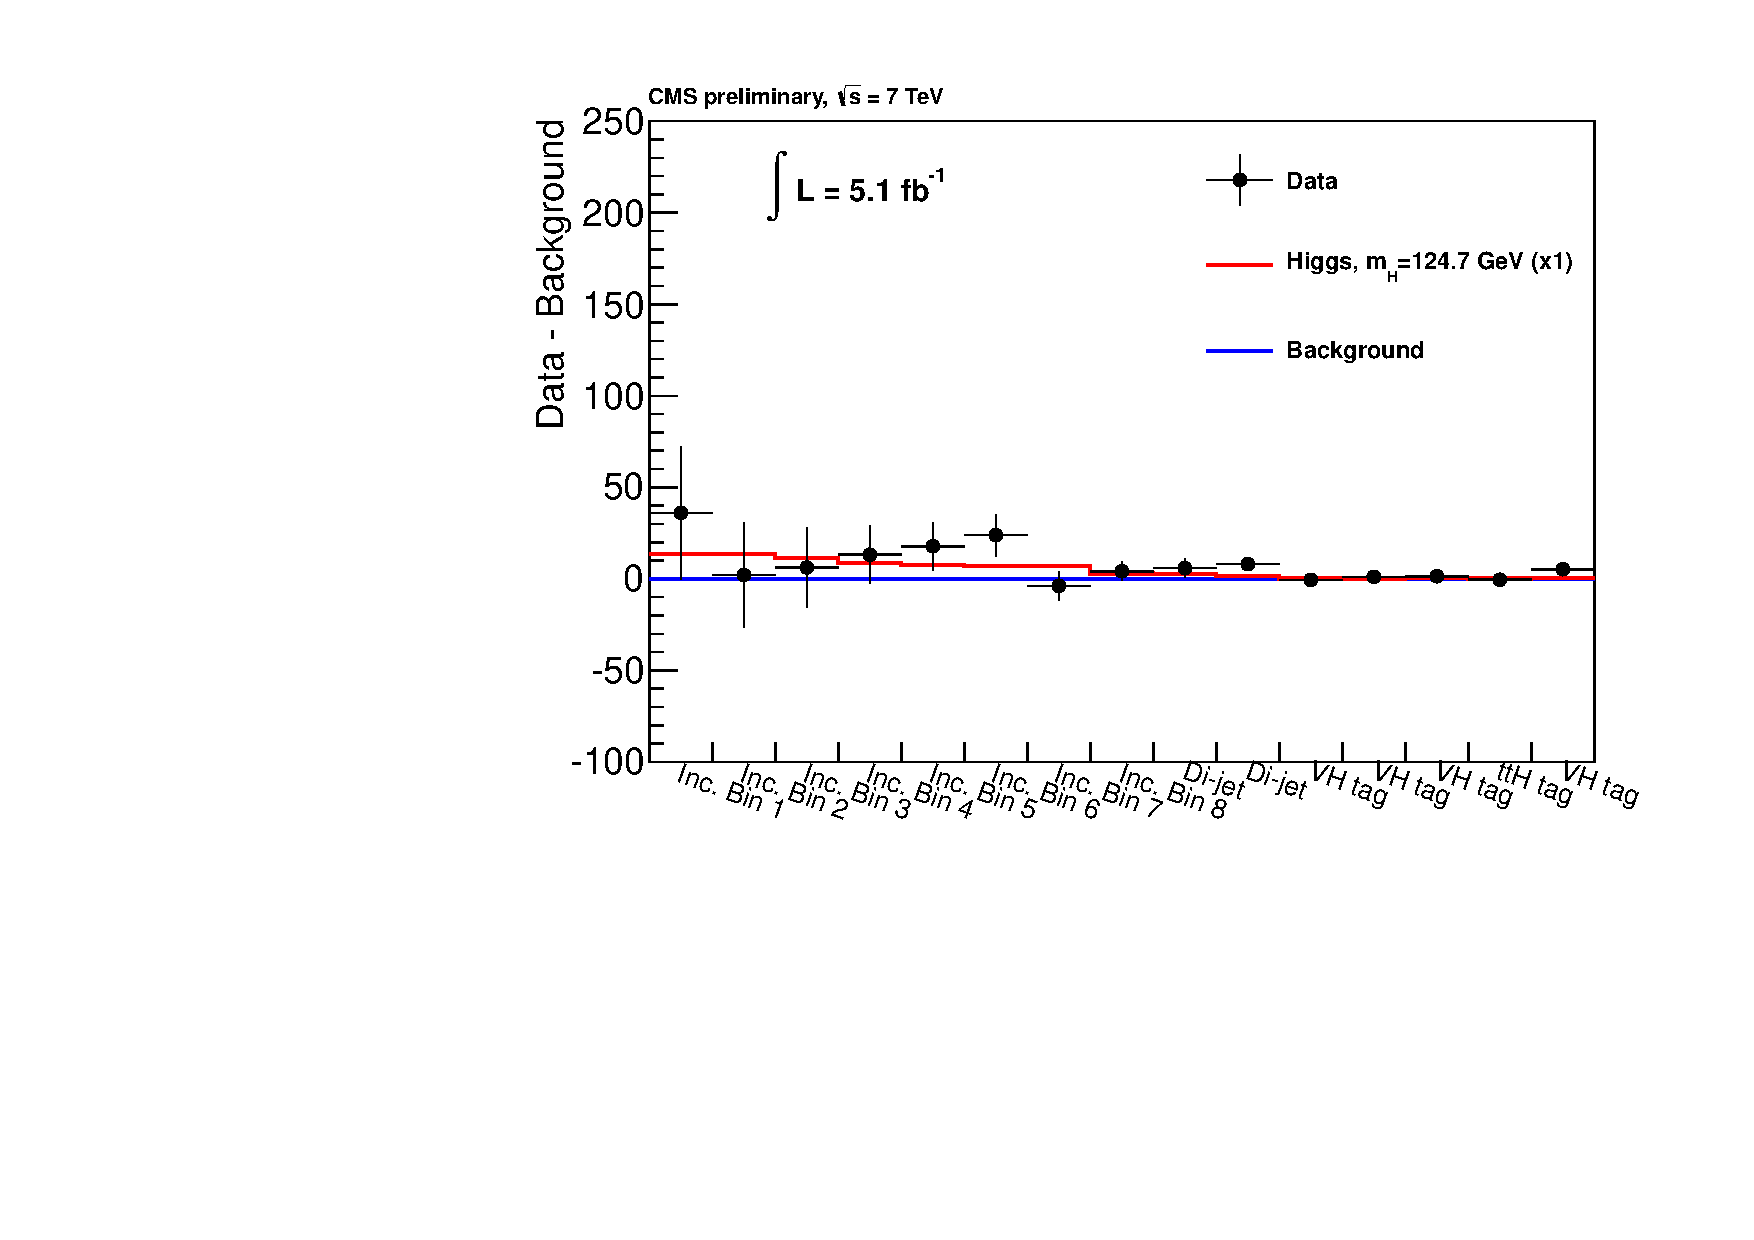
\includegraphics[width=0.48\textwidth]{{analysis/plots/sideband/diff_model_7TeV_m124.7}.pdf}
  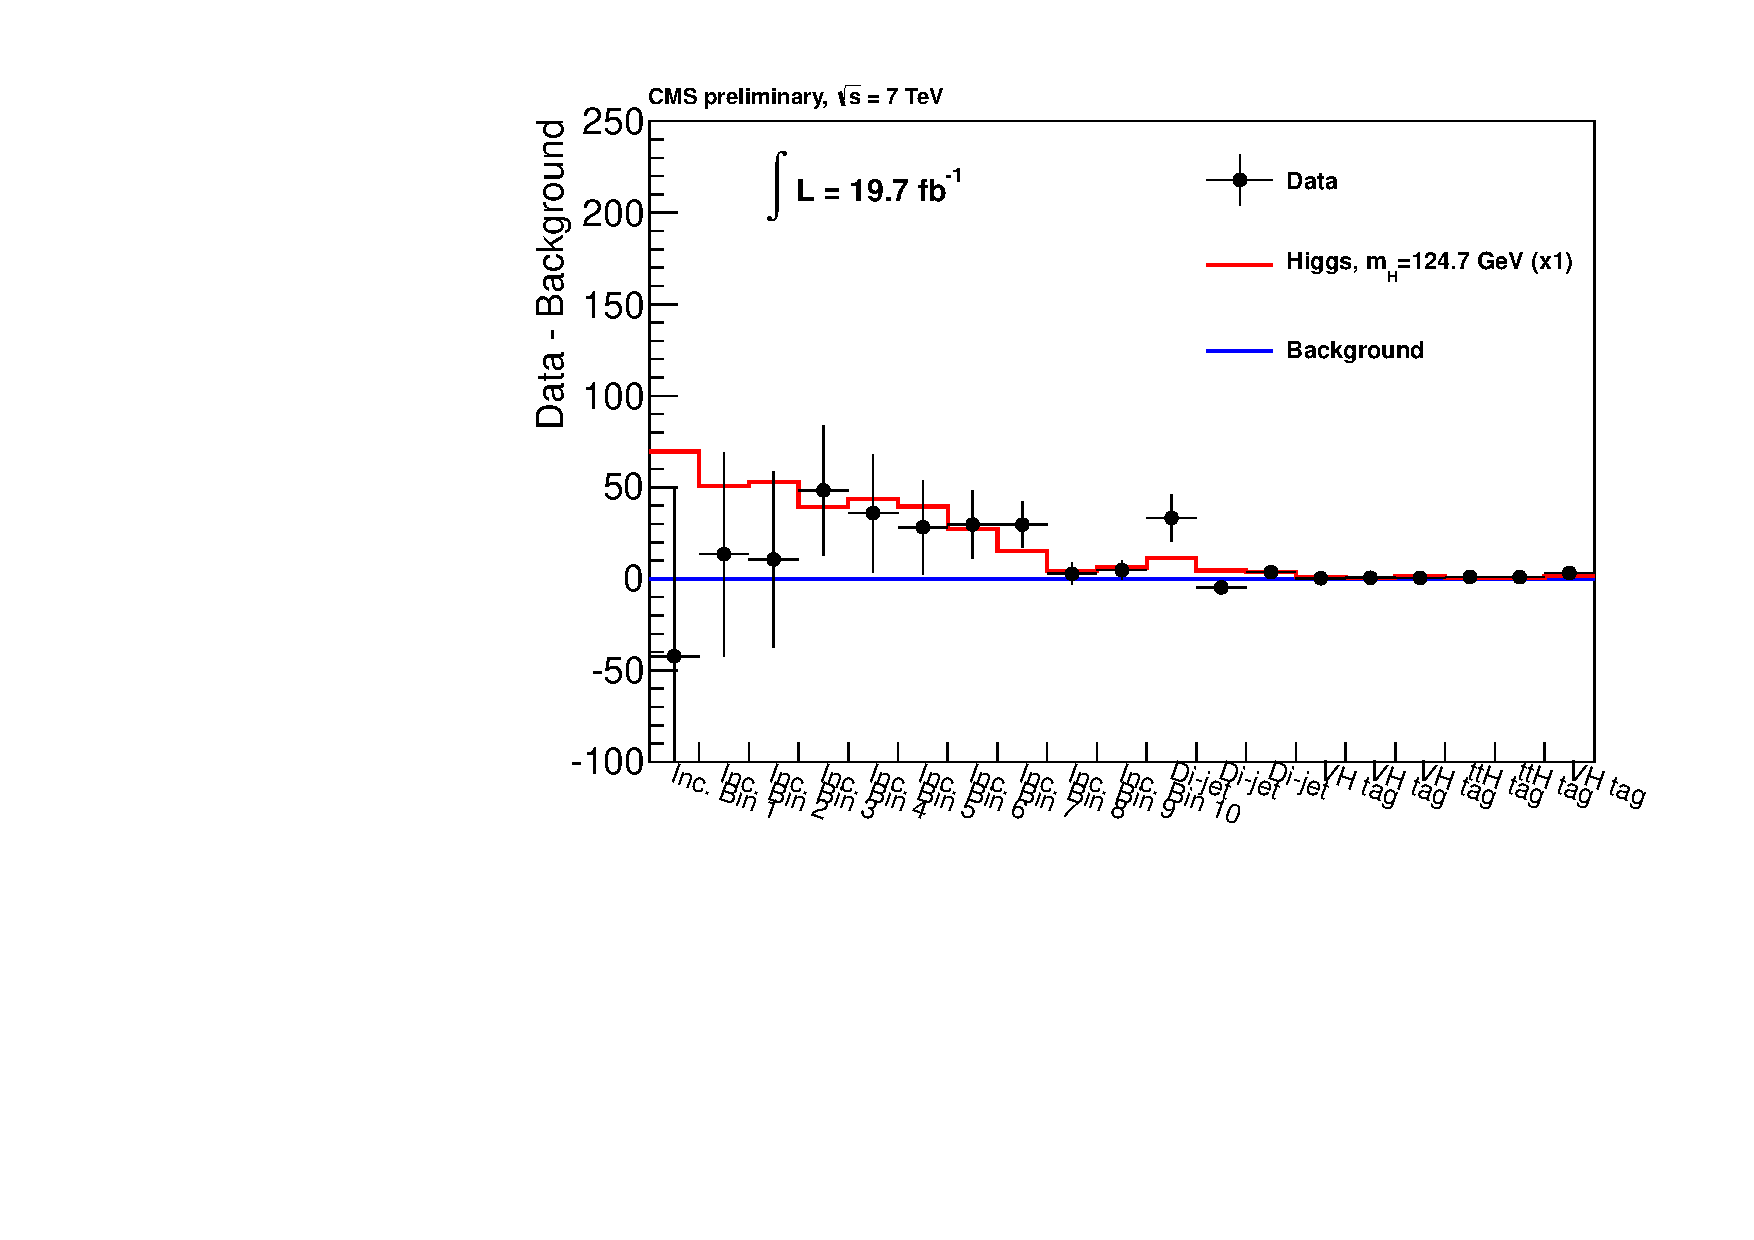
\includegraphics[width=0.48\textwidth]{{analysis/plots/sideband/diff_model_8TeV_m124.7}.pdf}
  \caption[The distribution of data, background and signal for the \SMVA]{The distribution in sideband analysis bins for the data (black points), the background (blue line), the error on the background (green and yellow bands) and the signal (red line) for the mass hypothesis at \mH=124.7~\GeV. The top row shows the expected number of events of each type for the 7~\TeV (left) and 8~\TeV (right) datasets. The bottom row shows the background subtracted plot for data (black points) and signal (red line).}
  \label{fig:sideband_output}
\end{figure}


% ---- SECTION ----
\section{Systematic Uncertainties}
\label{sec:systematics}

There are several sources of systematic uncertainty in the analysis and these are described in the following section. Nearly all of these affect the signal model, although there is an uncertainty associated to the ``envelope" background method, discussed in Sec.~\ref{sec:envelope}, for the \MFM and there are two uncertainties to the background for the \SMVA discussed separately below. The signal systematics come in three broad categories; those associated to individual photons, those associated to individual events and those associated to specific tagged event classes. The systematics get applied to the model in different ways depending on the level of correlation required between them. The \MFM analysis has a more precise correlation model between photon energy uncertainties and the mass shape, predominately because this is used for the main result and is required to provide a measurement of the observed bosons' mass. For the \SMVA this is somewhat simplified as the analysis only serves as a cross check of the categorisation and background estimation for which the important systematics are on the overall signal yield and not so much its shape or position. The way the systematics are implemented in the two analyses is explained below afterwhich there is a description of the individual uncertainties used. Their is a summary of the main groups of systematic uncertainty and their contribution to the uncertainty on the signal strength, $\sigma/\sigma_{\mathrm{SM}}$, in Table~\ref{tab:systematics_mu} and their contribution to the uncertainty on the mass measurement, \mH, in Table~\ref{tab:systematics_mh}, at the end of the section.

\subsection{Implementation of the systematic uncertainties}

\subsubsection{Mass Factorised Analysis}

In the \MFM uncertainties are implemented in two different ways. The first type are generally associated to the photon energy scale and resolution and the diffrences between photons and electrons. These are implemented as Gaussian nuisance parameters which affect the position, shape and normalisation of the signal probability distribution function. The second type are uncertainties which result in events being misclassified or cut out of the analysis. These are implemented as log normal nuisance parameters which affect the normalisation of the signal and the relative signal yield in each event class. Log normal constraints are chosen for the latter so that the nuisance term cannot go negative. These unceratinties are somewhat easier to understand as they simply dictate that events can migrate between categories and that the overall normalisation of the signal can vary due to the theoretical cross section, luminosity measurement etc. The former type is perhaps slightly harder to understand as these uncertainties are applied to individual photons and their effect is propagated through to the invariant mass shape and normalization of the signal for each production process and event class. The methodology for this is as follows,

\begin{itemize}
  \item Each uncertainty is designed to address a specific class of photons with similar properties. For example one uncertainty might be the energy scale uncertainty for unconverted photons in the barrel. We can label this class $c$ and the uncertainty for this class $\theta_{c}$ which is the nuisance parameter that enters the signal model.
  \item Within the class $c$ there may be several sub groups of photons which have different uncertainties. For example photons in the central barrel and outer barrel. We will label this uncertainty as $\sigma_{s}$.
  \item The full analysis is run through where each photon in class $c$ has its scale altered acorrding to a random Gaussian number centered on its nominal value with a width of its individual uncertainty $\sigma_{s}$ and all other photons left alone. 
  \item The distribution of the diphoton invariant mass shape for the signal is compared when the random shift above is applied and when it is not. The relative difference between the mean, effective width and overall rate of these two shapes is calculated, labelled $k_{\mu}$, $k_{\sigma}$ and $k_{r}$ respectively, for each signal process and analysis event class separately. This then provides a measure of the $1\sigma$ systematic effect on the signal mass shape of the uncertainty $\theta_{c}$.
  \item Given there are several nuisance parameters $\theta$ for which this is done, the signal model Gaussian parameters then get reparametrised as follows;
    \begin{flalign}
      & \mbox{Gaussian mean:} \;\;\;\;\; \mu(\mH) = \hat{\mu}(\mH)\Biggl(1+\displaystyle\sum_{c}k_{\mu c}\theta_{c}\Biggr) & \\
      & \mbox{Gaussian sigma:} \;\;\;\; \sigma(\mH) = \hat{\sigma}(\mH)\Biggl(1+\sqrt{\displaystyle\sum_{c}k_{\sigma c}^{2}\theta_{c}^{2}}\Biggr) & \\
      & \mbox{Signal rate:} \;\;\;\;\;\;\;\;\;\;\; r(\mH) = \sigma_{\mathrm{xs}}\cdot BR \cdot \epsilon\cdot\alpha \cdot L\Biggl(1+\displaystyle\sum_{c}k_{r}\theta_{c}\Biggr) &
    \end{flalign}
\end{itemize}

where $\hat{\mu}$ and $\hat{\sigma}$ represented the nominal fitted values of the Gaussians means and widths in the \MC.
The final event classes contain mixtures of photons from several different regions (in \eta and \rnine) which all have different associated uncertainties. Using this method the full correlation between the individual photon uncertainties is completey mapped onto the final invariant mass signal shape of each analysis category. 

\subsubsection{Sideband Analysis}

As the sideband analysis is simply a cut and count experiment across 15 (19) bins in the 7 (8)~\TeV datasets the uncertainties are just implemented as normalisation errors effecting the yield in each bin. These can arise from the energy scale, resolution, reconstruction efficiency etc.~and result in event migrations between bins or arise from the theoretical cross section, luminosity measurement etc.~and effect the overall signal normalisation. There are two systematics in the \SMVA associated to the background estimation from the sidebands. The first arises from the assumption that the background varies linearly across sidebands, although this has a neglible impact on the overall signal yield error. The second arises from the assumed shape used to extract the background normalisation. This is the dominant systematic in the analysis and is extracted using a bias study similar to the one described for the envelope method in Sec.~\ref{sec:envelope}. The size of this uncertainty is X\% (X\%) on the background rate in the 7 (8)~\TeV dataset.

\subsection{Systematic uncertainties related to individual photons}

\subsubsection{Photon energy scale}
In Section~\ref{sec:photon_energy} a method for correcting the photon energy using \Zee decays was described. Although the statistical uncertainties on these corrections is small, there are some data/\MC discrepancies that gives rise to a systematic uncertainty. This uncertainty is individually calculated for the 8 categories (4 in \eta and 2 in \rnine) for which the energy scale correction is applied. There are four nuisance parameters for each of the 7 and 8~\TeV datasets propagated to the signal model representing the energy scale uncertainty for barrel/endcap, converted/unconverted photons.

\subsubsection{Photon energy resolution}
Section~\ref{sec:photon_energy} also describes the method used to smear the \MC such that the energy resolution matches that observed in data using the \Zee control sample. As above there are four nuisance parameters representing the stocastic smearing uncertainty for each of the 7 and 8~\TeV datasets for barrel/endcap, converted/uncoverted photons. Additionally for converted/unconverted photons in the barrel there is an additional pair of uncertainties for the constant smearing term.

\subsubsection{Energy scale uncertainty due to differences between electron and photon reconstruction}
As the uncertainties, and the corresponding corrections, to the energy scale and resolution described above are derived from the \Zee decay an important source of systematic uncertainty arises from differences between electrons and photons which are not well modelled by the \MC. The effect which is most significant is due to an imperfect description of the tracker and servicing material between the beampipe and the \ECAL in the simulation. Studies of photon conversions, electron bremstraulung and pion scattering suggest a material defecit in the simulation of up to 10\% in some areas of the \ECAL. The uncertainty on the energy scale is assessed by using specialised \MC samples in which the tracking material budget is increased by 10\% and 20\% in 8 categories (4 in \eta and 2 in \rnine). Two nuisance parameters, which get correlated across the 7 and 8~\TeV datasets, are implemented representing the energy scale uncertainty due to the material mismodelling in the central barrel, $|\eta|<1$, and the rest of the barrel.

A futher difference between electron and photons which is not modelled in the simulation is the variation in the amount of scintillation light which reaches the photodetector given the longitudinal position in the crystal at which the light is emitted. Typically the peak position of the amount of scintillation light for electron showers is earlier in the crystal than photon showers and this is assumed as uniform in the simulation. A single correlated nuisance parameter is applied to account for this effect.

Finally one further systematic is applied to account for improvements made in more recent versions of the simulation which model electron bremstraulung at low \pT and photon conversion at high \pT much better. An additional correlated nuisance parameter is applied to account for this effect.

\subsubsection{Photon preselection efficiency}

The efficiency of the preselection described in Sec.~\ref{sec:photon_presel} is measured using \Zee decays in data and \MC. The \MC efficiency is then corrected such that it matches the data and this incurs a systematic uncertainty which gets applied as an overall normalization on the expected signal event yield in each analysis category. 

\subsubsection{Photon identification BDT}

The photon identification BDT output (described in Sec.~\ref{sec:pho_id_mva}) is an important input to the diphoton BDT which is used to classify events. A shift in the photon ID BDT output, due to inaccurate simulation in the training samples, can have a direct effect on the ouput of the diphoton event BDT which in turn will lead to an event being misclassified; either it will fail the lower edge cut or it will go into a different analysis category. By examining the variation in the photon ID output for \Zee electrons, \Zmumugamma photons and diphoton events in data with \mgg>160~\GeV it is found that applying a systematic shift of 0.01 to the output covers any discrepancies between data and \MC. This shift is applied and then propagated through to the diphoton \BDT which in turn results in an uncertainty implemented as relative yield change across event class (in other words a category migration).

\subsubsection{Photon resolution estimate}

The most imporant input to the diphoton BDT, the variable with the most discriminating power, is the photon energy resolution estimate. As for the photon ID systematic above the differences between data and \MC are studied for \Zee decays, \Zmumugamma decays and high \pT photons and a systematic variation of $\pm10$\% of the nominal value adequately covers any discrepancy. This variation is applied to photons and then propagated through to the diphoton \BDT and as above is implemented as an event migration uncertainty.

\subsection{Systematic uncertainties related to diphoton events}

\subsubsection{Vertex efficiency}

The vertex efficiency in \MC is corrected by a scale factor obtained from the vertex efficiency ratio between data and \MC as measured in \Zmumu events where the muon tracks are ignored (to replicate the situation with photons). The uncertainty associated to this is implemented by changing the relative fraction of the right/wrong vertex signal shape. 

\subsubsection{Trigger efficiency}

The trigger efficiency in \MC is corrected to match the data using \Zee events with a tag and probe technique~\cite{tag_and_probe}. The uncertainty associated to this is implemented as an overall normalisation change in each category.

\subsubsection{Mass scale non-linearity}

Another important consideration when using the \Zee decay as a calibration and control tool in the analysis is not only the differences between electrons and photons but also the difference in the mass scale between the $Z$ ($m_{Z}=91.2$~\GeV~\cite{pdf}) and a Higgs boson at \mH=125~\GeV. Although the absolute difference is not imporant, the respective differences between data and \MC are. This effect is measured by comparing the energy measured from the eleromagnetic shower alone and the \pT from the tracker of electrons as a function of the scalar \ET sum of the two electrons in \Zee decays. This uncertainty is applied as global mass shift, independently in the 7 and 8~\TeV datasets, which has a correlated effect on the signal position in each category.

\subsubsection{Luminosity measurement}

The luminosity measurement and its uncertainty is a \CMS universal value and described in Refs.~\cite{lumi1,lumi2}.

\subsubsection{Theoretical cross section and branching ratio}

The uncertainties on the theoretically predicted \SM Higgs cross section and its branching fraction to two photons are implemented following the recommendations of the LHC Higgs Cross Section Working Group~\cite{LHCHiggsCrossSectionWorkingGroup3}. 

\subsection{Systematic uncertainties related to production mode tagged classes}

\subsubsection{Jet tagging efficiency}

One of the largest uncertainties for measurement of the respective couplings to fermions and bosons of the Higgs boson originates from the complexity in isolating events produced by gluon fusion and those produced by vector boson fusion. As described in Sec.~\ref{sec:exclusive_tags} this is done by tagging jets characteristc of \VBF Higgs decays however there is a large uncertainty involved when additional jets are produced by gluon fusion induced Higgs decays. Using the Stewart-Tackmann procedure~\cite{vbf_syst} the uncertainty on the yield of gluon fusion events in the \VBF tagged event classes is calculated and implemented as a category migration systematic. There are futher effects from the jet energy scale, jet id efficiency and the efficiency of rejecting pile up jets from geniune particles which are taken from Refs.~\cite{jet_energy_corrections,jet_energy_corrs2}. These effect the relative yields of the signal expectation between the \VBF categories and also from the \VBF categories as a whole to the inclusive categories.  

\subsubsection{Lepton, \MET and $b$-tagging efficiency}
Additional normalisation uncertainties are applied to the exclusive mode categories which account for the efficiency of reconstructing and tagging leptons, \MET and $b$-jets.

\subsection{Summary}

\begin{table}[htbp]
\caption[Magnitude of the uncertainty on the signal strength, $\musm$, induced by the systematic uncertainties on the signal]{Magnitude of the uncertainty on the signal strength, $\musm$, induced by the systematic uncertainties on the signal. These are not final numbers. Would also be nice to have plot of asimov likelihood curve of expected signal strength when adding different components in.}
\begin{center}
\begin{tabular}{ l c }
\hline
\multirow{2}{*}{\textbf{Systematic uncertainty}} & \textbf{Uncertainty} \\
 &  \textbf{on $\musm$} \\
\hline
\hline
%%%%%% per photon ----------------
Energy resolution, scale and resolution estimation & 0.04\\
\hline
Trigger, photon preselection, and vertex finding efficiencies& 0.02\\
\hline
Uncertainties specific to tagged classes & 0.02\\
\hline
Production cross sections, branching fractions, and integrated luminosity & 0.12\\
\hline
\hline
All systematic uncertainties on signal model & 0.15 \\
\hline
\end{tabular}
\end{center}
\label{tab:systematics_mu}
\end{table}

\begin{table}[htbp]
\caption[Magnitude of the uncertainty on the signal position, $\mH$, induced by the systematic uncertainties on the signal]{Magnitude of the uncertainty on the signal position, $\mH$, induced by the systematic uncertainties on the signal. These are not final numbers. Would also be nice to have plot of asimov likelihood curve of expected signal strength when adding different components in.}
\begin{center}
\begin{tabular}{ l c }
\hline
\multirow{2}{*}{\textbf{Systematic uncertainty}} & \textbf{Uncertainty} \\
 &  \textbf{on $\mH$} \\
\hline
\hline
%%%%%% per photon ----------------
Energy resolution, scale and resolution estimation & 0.02\% \\
\hline
Non linearity extrapolation from $Z$-boson scale to Higgs scale & 0.07\% \\
\hline
Differences between electrons and photons & 0.08\% \\
\hline
\hline
All systematic uncertainties on signal model & 0.12\% \\
\hline
\end{tabular}
\end{center}
\label{tab:systematics_mh}
\end{table}

\section{Statistical interpretation of the data}
\label{sec:stats}
To aid with statistical interpretation of the data it is useful to define two hypotheses to which the data can be compared. These are the background only model and the signal plus background model known as the null hypothesis, $H_{0}$, and the alternate hypothesis, $H_{1}$, respectively. The background model is obtained from the data by profiling the different parametrisation choices, as per the ``envelope" method described in Sec.~\ref{sec:envelope}. The benchmark used for the signal model is the \SM Higgs expectation as described in Sec.~\ref{sec:signal_model} which can be expressed in terms of the two physical parameters of interest; the signal strength relative to the \SM expectation, $\mu=\musm$, and the signal position or Higgs mass, \mH. The likelihood function for statiscal interpretation can be written as,
\begin{equation}
  \mathcal{L}(\mu,\mH;\theta,\theta_{d}|\mgg) = \mu\cdot\mathbf{S}(\mgg|\mu,\mH;\theta) + \mathbf{B}(\mgg|\theta_{d}),
  \label{eq:likelihood}
\end{equation}
where \mgg is the diphoton invariant mass, $\theta$ are continuous nuisance parameters effecting the signal model, $\theta_{d}$ are discrete nuisance parameters effecting the background model and $\mathbf{S}$ and $\mathbf{B}$ are the probability distribution functions for the signal and background repsectively. In the case of the \SMVA there is no dependence on \mgg as events are simply counted in the analysis bins. It can be seen that $\mu$ is continuous parameter which represents the size of the fitted signal. The null hypothesis, or background only model, is a simple case of the full model where $\mu=0$.

When determining the best fit values of parameters in our model and their errors the full likelihood function, as expressed in Eq.~\ref{eq:likelihood}, is fit to the data and the \NLL is scanned as a function of the parameter(s) of interest. This is a standard statistical procedure for measuring the value and error of a model parameter~\cite{FredJames}. An important measurement to make of the Higgs boson is its relative coupling to fermions and bosons respectively. Given that the signal model is expressed as a sum over the different production processes one can redefine the likelihood in this case so that the signal strength is split into two coupling strength parameters, $\mu_{\mathrm{fermions}}$ and $\mu_{\mathrm{bosons}}$.

\begin{align}
  \mu\cdot\mathbf{S}(\mgg|\mu,\mH;\theta) & = &  \mu_{\mathrm{fermions}}\cdot\biggl(\mathbf{S_{ggH}}(\mgg|\mu,\mH;\theta)+\mathbf{S_{ttH}}(\mgg|\mu,\mH;\theta) \biggr) \nonumber \\
 & & + \mu_{\mathrm{bosons}}\cdot\biggl(\mathbf{S_{qqH}}(\mgg|\mu,\mH;\theta)+\mathbf{S_{VH}}(\mgg|\mu,\mH;\theta)\biggr)
 \label{eq:rvrf}
\end{align}

where $\mathbf{S_{proc}}$ represents the signal model for the process ``proc" only.

There are two important statistical tests that get performed aside from ascertaining the best fit values of parameters in the model. The first is an exclusion test designed to reject the alternate hypothesis in data. The second is a probability, or $p$-value, test designed to ascertain the likelihood of the null hypothesis fluctuating to give a signal. This requires definition of a test statistic,
\begin{equation}  
  q_{\mu} = 
  \begin{cases}
    -2\ln\frac{\mathcal{L}(\mathrm{data}|\mu,\mH,\hat{\theta}_{\mu})}{\mathcal{L}(\mathrm{data}|\hat{\mu},\mH,\hat{\theta}_{\hat{\mu}})} & 0\leq\hat{\mu}\leq\mu \\
    0 & \hat{\mu}<0
  \end{cases}
  \label{eq:teststat}
\end{equation}
where $\hat{\theta}_{\mu}$ and $\hat{\theta}_{\hat{\mu}}$ represent the nuisance parameters at their best fit values given a particular value of \mu and given \mu is freely floating and at its global best fit value $\hat{\mu}$. The statistical tests which require $q_{\mu}$ are carried out at a specific hypothesised Higgs mass and so \mH is set to a particular value when defining the test statistic. It can be shown that $q_{\mu}$ is the most powerful test of hypothesis $H_{0}$ against hypothesis $H_{1}$ and this is known as the \textit{Neymann-Pearson Lemma}~\cite{FredJames}.

For exclusion limits the $CL_{s}$ method is used, which is desgined to give less stringent limits in situations where there is little discriminatory power between the null and alternate hypotheses~\cite{cls}. The $CL_{s}$ exclusion requires caluclation of two p-values given the test statistic distribution of the two hypotheses is known, as shown in~\cref{eq:cls1,eq:cls2,eq:cls3}. A common way of obtaining this distribution is by generating pseudo-data under each hypothesis however at \CMS asymptotic approximations are used to avoid the computational overhead of generating toys~\cite{asymptotic_form}. A one sided upper limit is determined on $\mu$ by enforcing the constraint that $\hat{\mu}\leq\mu$ and the exclusion power of the limit is given by 1-$CL_{s}$. The defintion of the $CL_{s}$ is, 

\begin{align}
  & CL_{s} = \frac{CL_{s+b}}{CL_{b}} \label{eq:cls1}, \\
  & CL_{s+b} = \int_{q_{\mu}^{obs}}^{\infty}f(q_{\mu}|\mu=\hat{\mu})dq_{\mu} \label{eq:cls2}, \\
  & CL_{b} = \int_{q_{\mu}^{obs}}^{\infty}f(q_{\mu}|\mu=0)dq_{\mu} \label{eq:cls3}, 
\end{align}

where $q_{\mu}^{obs}$ is the observed value of the test statistic in data and $f(q_{\mu}|\mu)$ is the distribution of the test statistic for the hypothesis with value $\mu$. The $CL_{s}$ exclusion method is demonstrated by an example in Fig.~\ref{fig:cls}. In this case a \SM Higgs boson with values of signal strength $\mu>0.8$ is excluded at 92.48\%. In reality the desired exclusion level is 95\% and consequently the value of $\mu$ is adjusted until the $CL_{s}$ reaches 0.05 and then all values of $\mu$ greater than or equal to this value are considered as excluded. When referring to the ``expected" exclusion (as opposed to the ``observed" exclusion just explained) the observation value is considered as being at the mean of the null hypothesis test statistic distribution.

\begin{figure}
  \begin{center}
    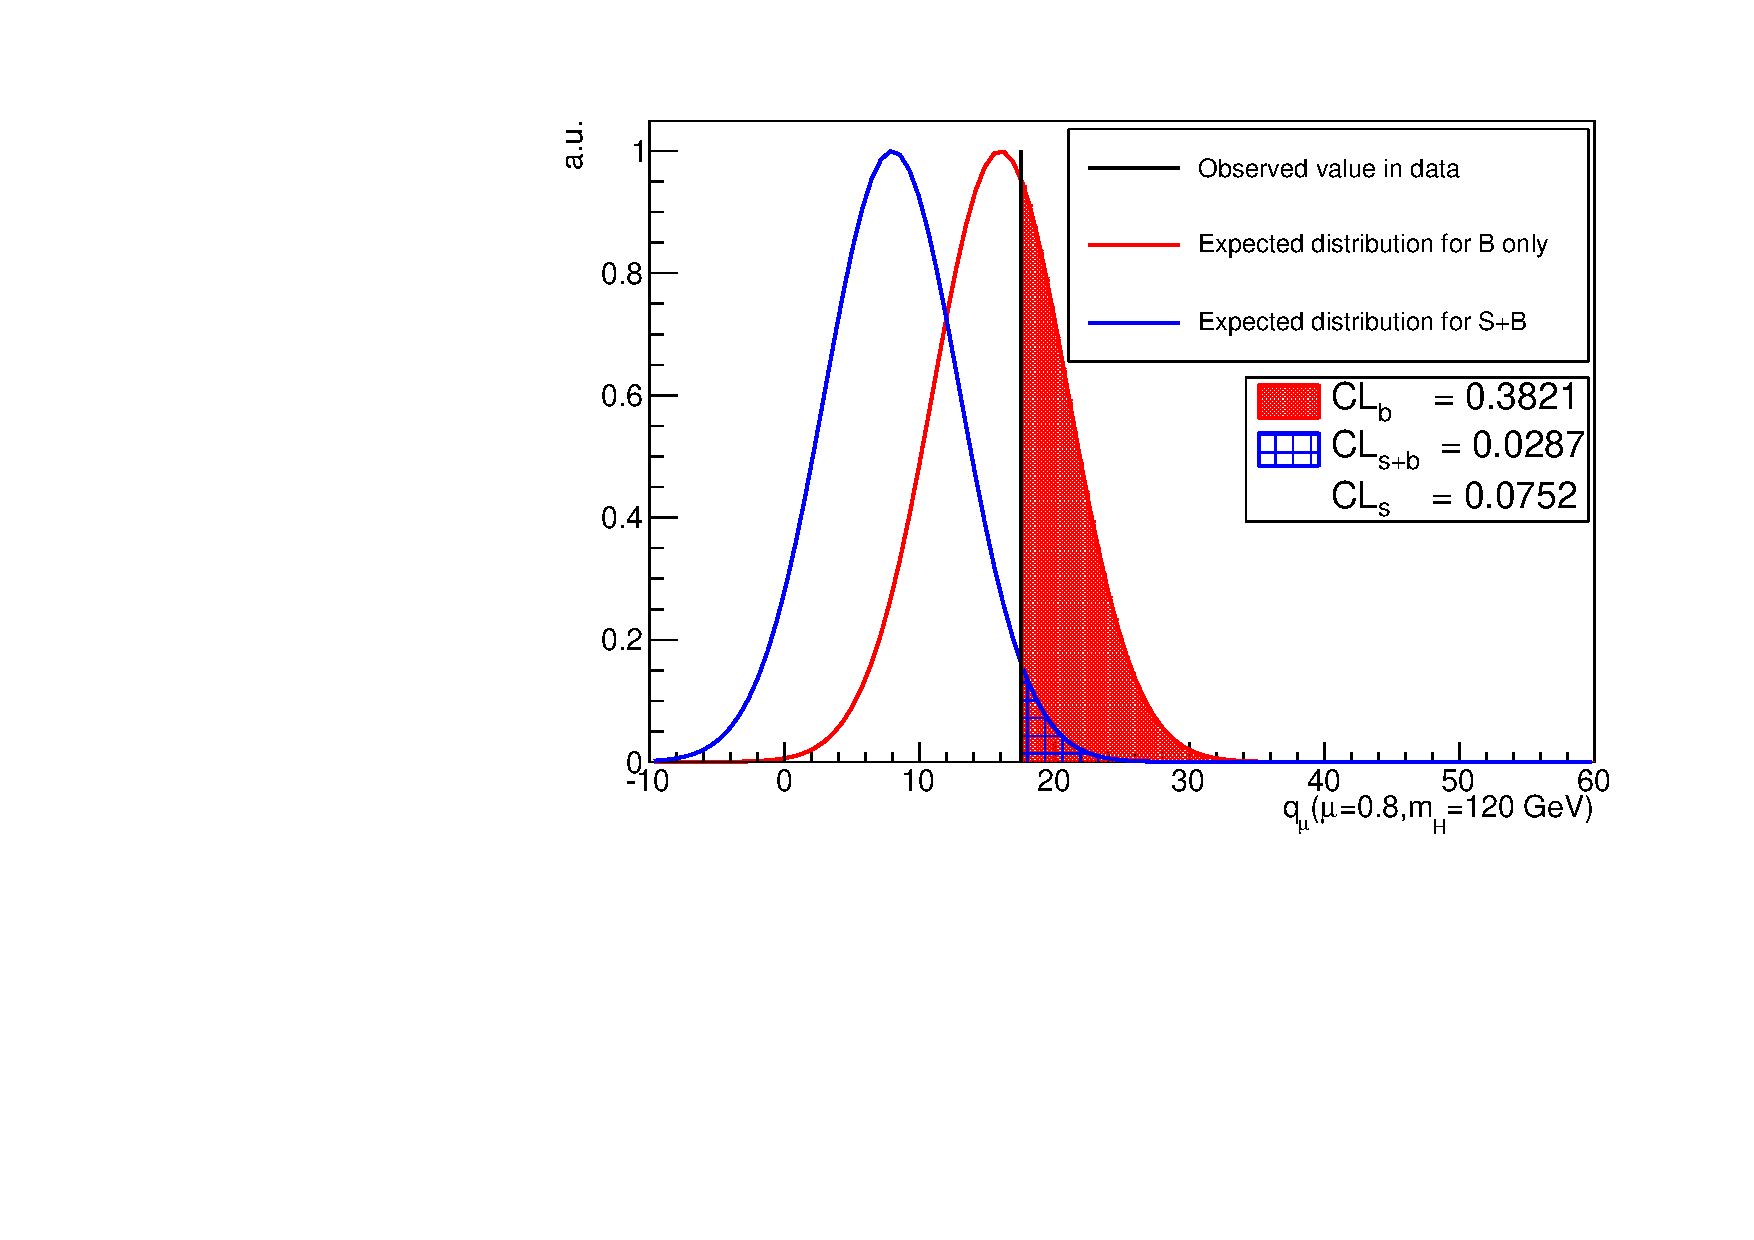
\includegraphics[width=0.8\textwidth]{analysis/plots/testStatDrawing.pdf}
    \caption[A demonstration of the test statistic distribution]{A demonstration of the test statistic distribution for the background only model (red) and the signal plus background model (blue) and the observed value in data (black line). The exclusion power is given by 1-$CL_{S}$, in this case values of $\mu>0.8$ are excluded at 92.48\% confidence.}
    \label{fig:cls}
  \end{center}
\end{figure}

When quantifying the significance of an observed excess the test statistic $q_{0}$ is used which is obtained by setting $\mu=0$ in Eq.~\ref{eq:teststat}. The requirement that $\hat{\mu}\geq0$ ensures that only positive excesses are considered significant. The probability that the background only hypothesis is rejected in favour of the signal plus background hypothesis is given in terms of the $p$-value, $p_{0}$, defined as,
\begin{equation}
  p_{0} = \int_{q_{0}^{obs}}^{\infty}f(q_{0}|\mu=0)dq_{0}.
  \label{eq:pvalue}
\end{equation}
Typically a value of $p_{0}\leq1.3\times10^{-3}=3\sigma$ is enough to claim observation of new physics while $p_{0}\leq2.87\times10^{-7}=5\sigma$ is enough to claim a discovery of new physics.

\section{Spin analysis}
\label{sec:spin}

The Landau-Yang theorem forbids the direct decay of a spin-1 particle into a pair of photons~\cite{Landau1948,Yang1950}. 
Consequently the spin analysis compares the expectation of the spin-0 SM Higgs, \zerop, and the spin-2 \emph{graviton-like} 
model with minimal couplings, \twomp,~\cite{Gao2010}. The \twomp graviton resonance is produced in one of two ways, gluon-fusion ($gg$) 
or quark-antiquark annihilation (\qqbar). This chapter presents hypothesis tests between the \zerop and the \twomp varying the the amount of 
\twomp production from \qqbar. For the \zerop SM 
resonance all production modes have been considered; \ggH, \VBF, \WH, \ZH, \ttH. 

As the \twomp is just one of many spin-2 models it is desirable to make the analysis as model independent as possible. As a means of 
discriminating the two hypotheses we use the scattering angle in the Collins-Sopper frame, \costhetastar ~\cite{CollinsSoper1977}, which is defined as the angle, in the diphoton rest frame, between the collinear diphotons 
and the line which bisects one incoming beam with the negative of the other beam, 
\begin{equation}
  \cos(\theta^{\ast}_{\mbox{\tiny{CS}}}) = 2\times\frac{E_{2}p_{z1}-E_{1}p_{z2}}{m_{\gamma\gamma}\sqrt{m^{2}_{\gamma\gamma}+p^{2}_{T\gamma\gamma}}},
\end{equation}
where $E_{1}$ and $E_{2}$ are the energies of the leading and trailing photon, $p_{z1}$ and $p_{z2}$ are the $z$-component momenta 
of the leading and trailing photon and $m_{\gamma\gamma}$ and $p_{T\gamma\gamma}$ are the invariant mass and transerve momenta of the diphoton system.

In its rest frame the photons from the decay of a spin-0 boson are isotropic. Hence prior to acceptance cuts, the distribution of \costhetastar 
under the \zerop hypothesis is uniformly flat. In general this is not the case for spin-2 decays. 

In order to reduce any model dependence in the analysis the cut based photon selection, described in Sec.~\ref{sec:cic}, is used to pick events. The \MVA methods used for event selection in the nominal analysis use specific \SM \MC training samples and most importantly one of the training variables used, namely $\cos(\phi_{1}-\phi_{2})$, is highly correlated to the angular variable, \costhetastar, which can be used to distinguish spin hypotheses. Furthermore, given the unusual production modes of a spin-2 boson, no exclusive tagging is used in the spin analysis. The impact of using jet variables was studied but it was found that the sensitivty for distinguishing spin hypotheses was improved by a neglible amount.

Two statistical tests are carried out in the spin analysis:

\begin{enumerate}
  \item The signal strength, $\mu$, is extracted differentially in bins of \abscostheta. This is a relatively model independent test and in principal allows any spin model to be compared to the data.
  \item The statistical separation between different spin hypotheses is calculated using a test statistic similar to the one described in Sec.~\ref{sec:stats} and the $CL_{s}$ exclusion method is used to quantify the separation power. This is a highly model dependent test but allows for the exclusion of specific spin models.
\end{enumerate}

\subsection{Event categorisation}
\label{sec:spin_cats}

%Preceding the cut based selection mentioned in section \ref{sec:photonID} and described in Ref.~\cite{HIG-13-001}, photons
%are preselected requiring, $p_{T}/m_{\gamma\gamma}>1/3$ ($p_{T}/m_{\gamma\gamma}>1/4$) for the leading (subleading) photon and
%$|\eta_{\mbox{\tiny{cluster}}}|<2.5$ for all photons, where $p_{T}$ is the transverse momentum of a photon, $m_{\gamma\gamma}$ is the diphoton invariant mass and $|\eta_{\mbox{\tiny{cluster}}}|$ is the pseudorapidity of the photon supercluster. In addition photons are rejected whose supercluster lies within the barrel-endcap transition region, $1.4442<|\eta_{\mbox{\tiny{cluster}}}|<1.566$.
The effect of the photon selection cuts on the distributions of 
\abscostheta is illustrated in Fig.~\ref{fig:acc_cuts}. Before any acceptance cuts, Fig.~\ref{fig:acc_cuts} (left), the \abscostheta
distribution of the \zerop processes is flat. This is not the case for the \twomp processes (gluon-fusion and quark-antiquark annihilation). After the selection cuts are applied these distributions are considerably distorted, Fig.~\ref{fig:acc_cuts} (right). As a Higgs produced from vector-boson-fusion, which is $\sim$8\% of the total (compared to $\sim$88\% from gluon fusion),  is typically produced at higher transverse momentum there is some additional contribution of \zerop signal at high values of \abscostheta compared to the \twomp production modes after the selection cuts.

\begin{figure}
	\begin{center}
	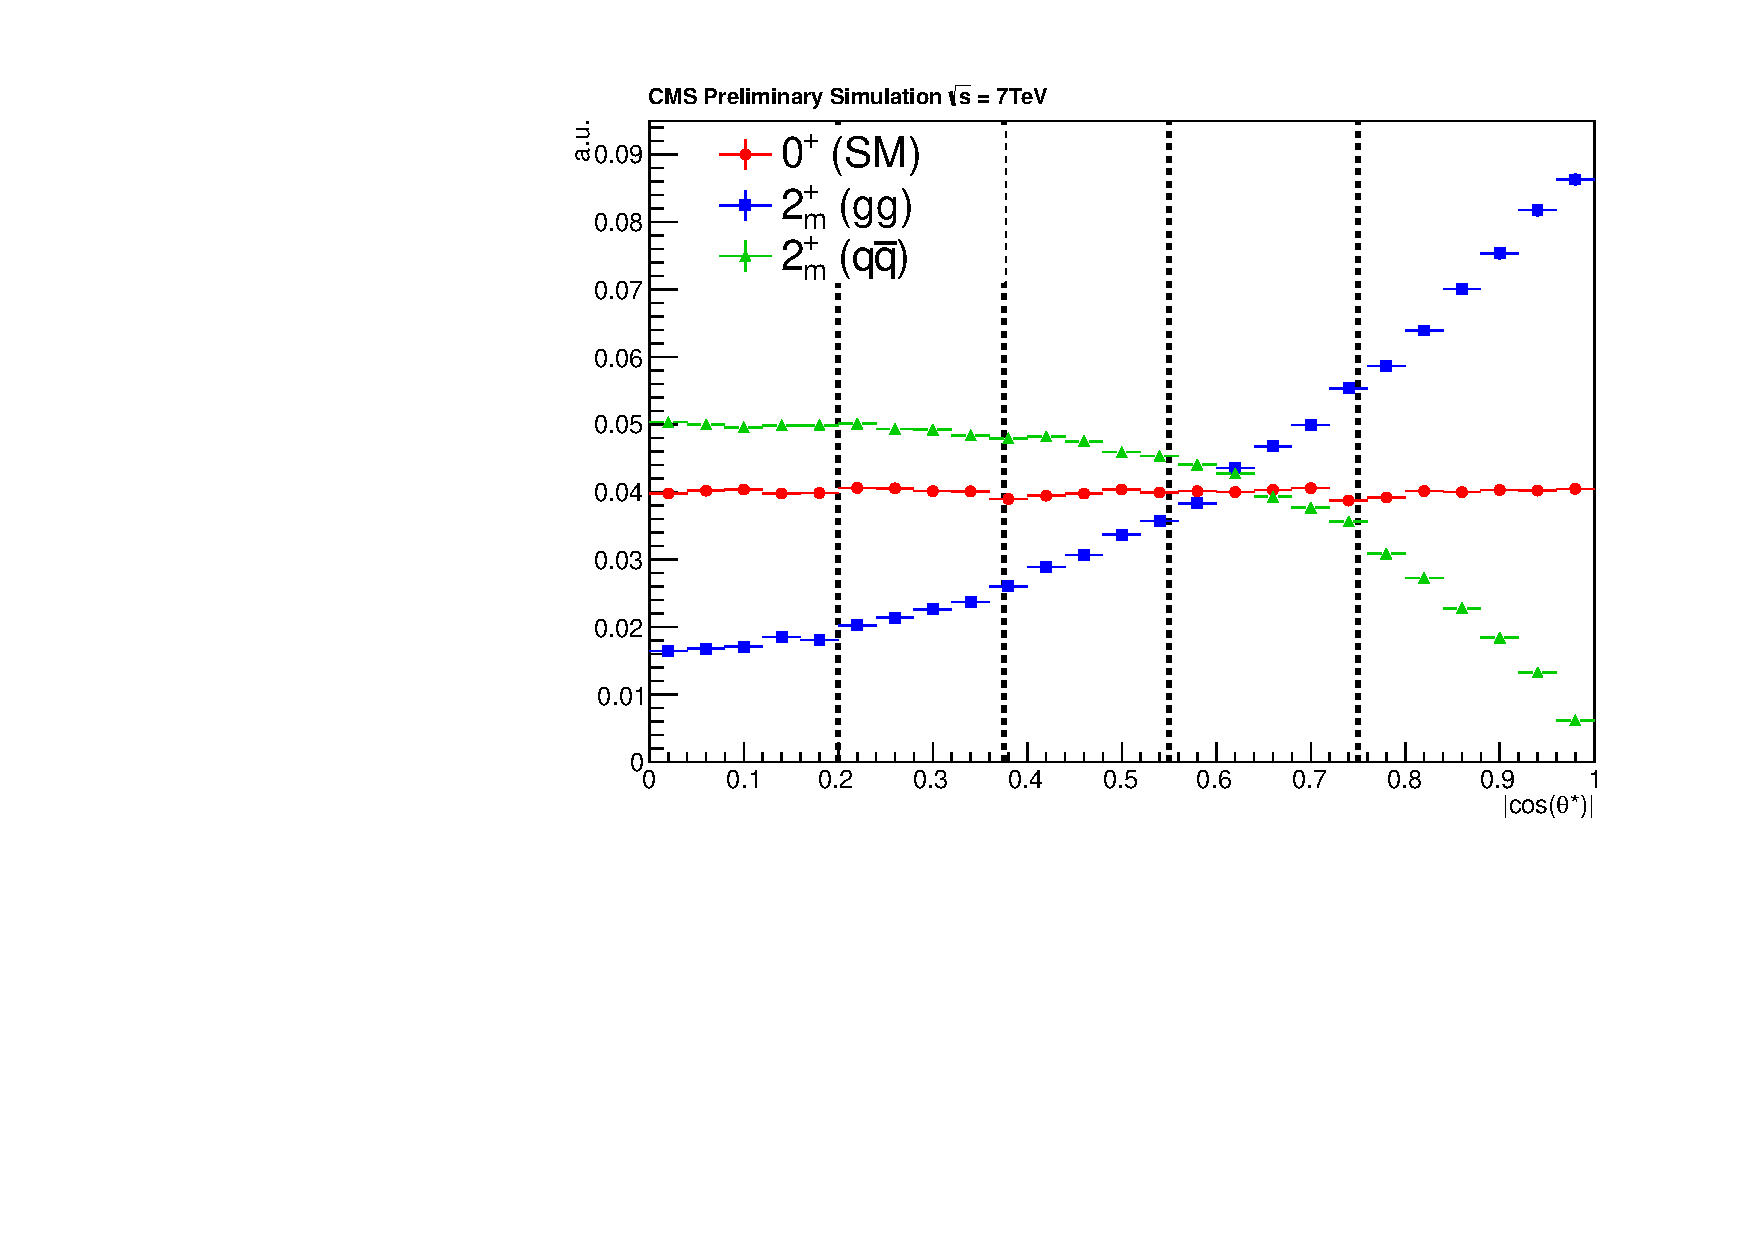
\includegraphics[width=0.49\linewidth]{spin/plots/before_7TeV.pdf}
	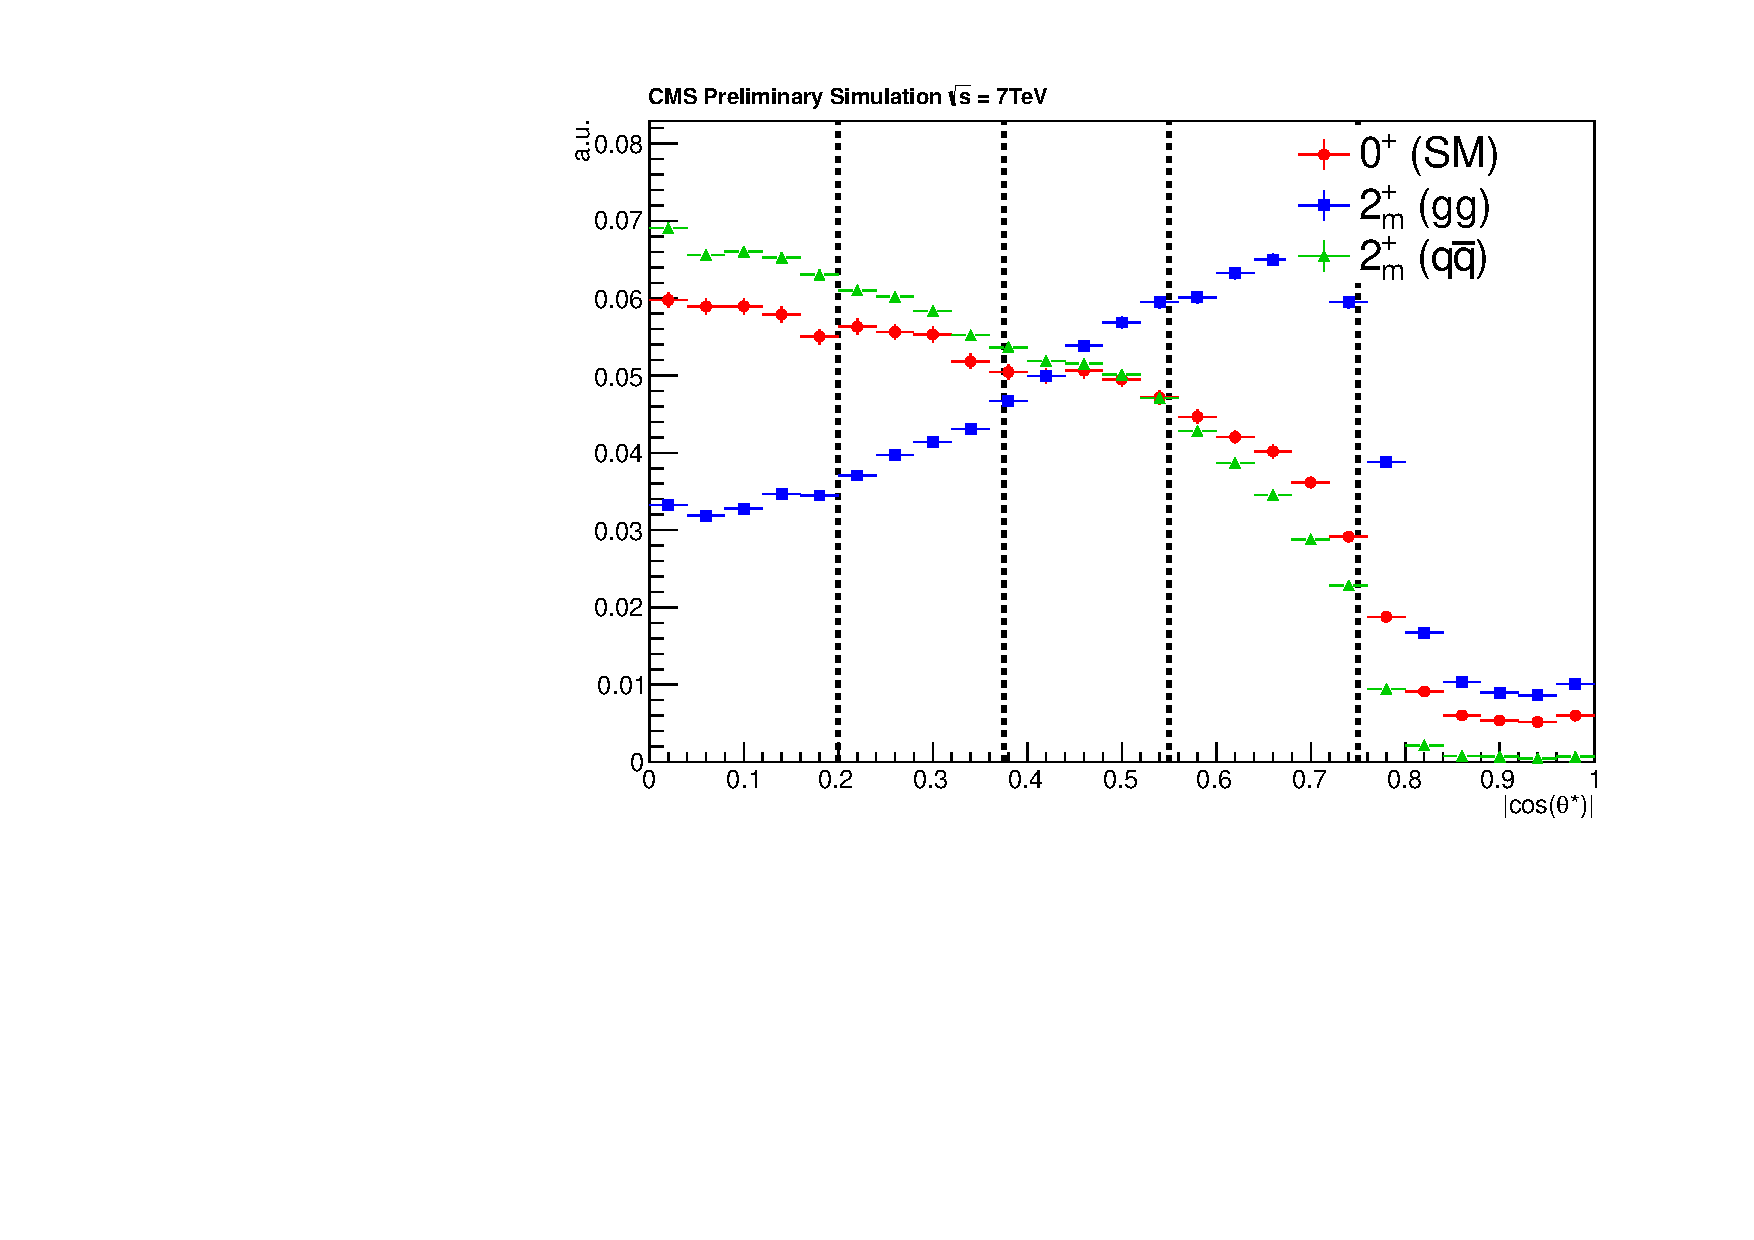
\includegraphics[width=0.49\linewidth]{spin/plots/after_7TeV.pdf} \\
	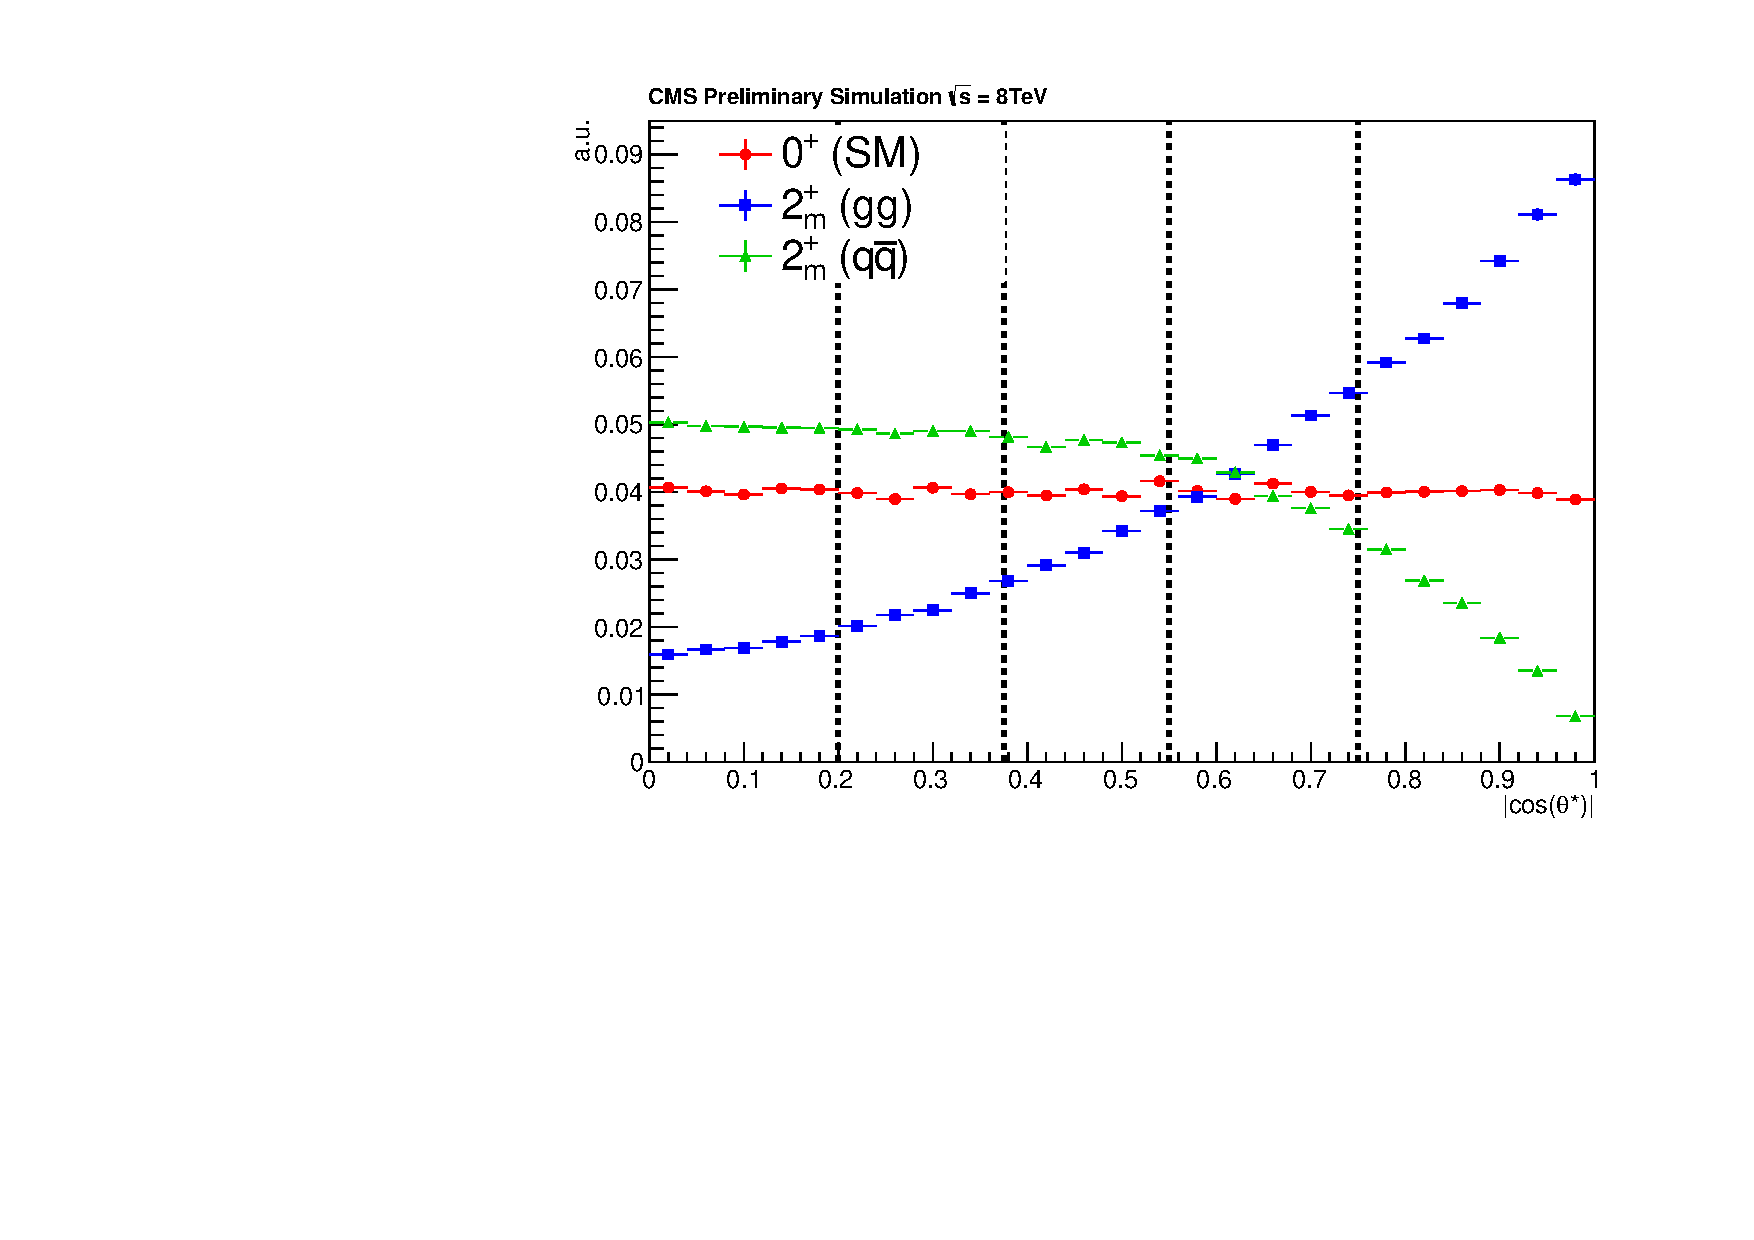
\includegraphics[width=0.49\linewidth]{spin/plots/before_8TeV.pdf}
	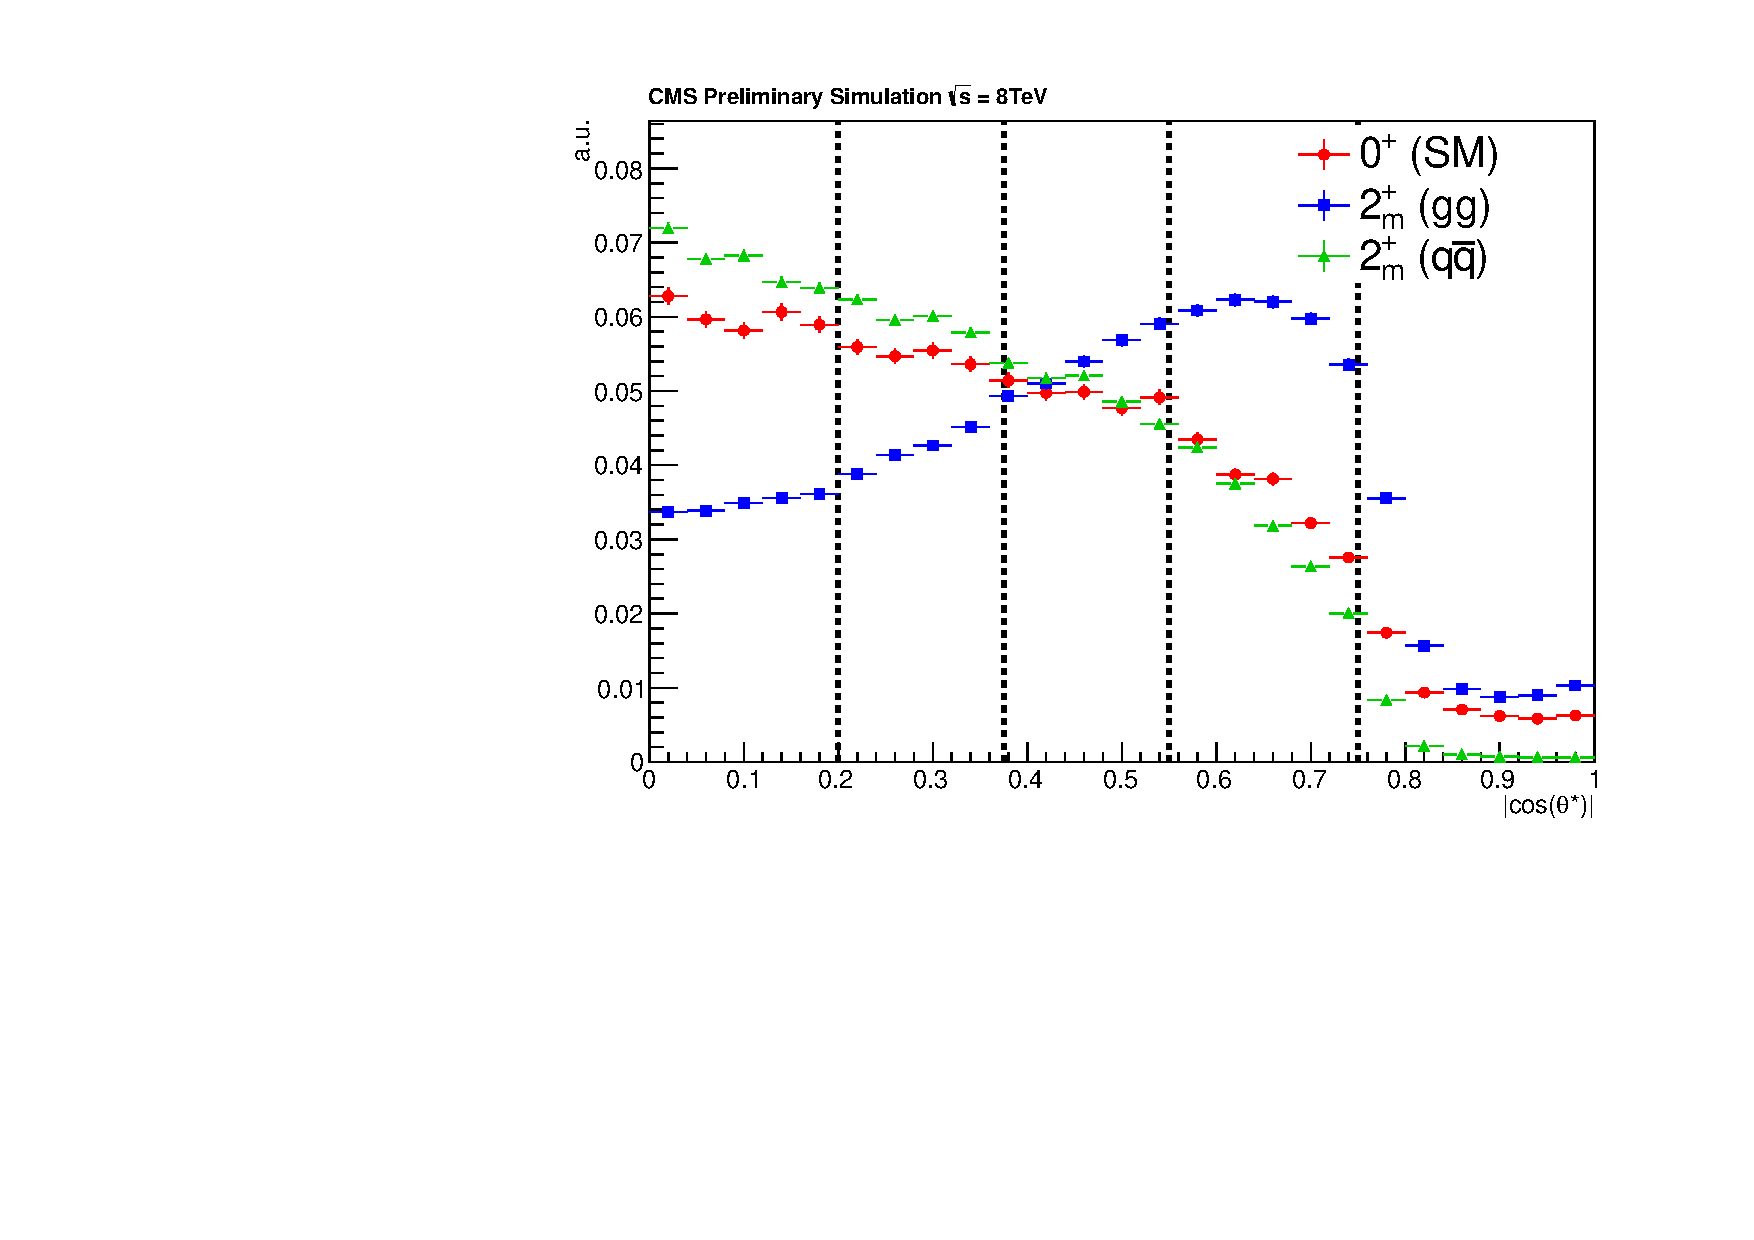
\includegraphics[width=0.49\linewidth]{spin/plots/after_8TeV.pdf} \\
	\caption[The distribution of \abscostheta before and after selection cuts for different spin signals]{The distribution of \abscostheta before any selection cuts (left) and after the selection cuts (right) for the 7~\TeV dataset top row and the 8~\TeV dataset bottom row. The three histograms represent the spin $0^+$ distribution with all SM production modes (red circular points), the spin $2^+_m$ distribution with the gluon-fusion production mode (blue square points) and the spin $2^+_m$ distribution with the quark-antiquark annihilation production mode (green triangular points). The \abscostheta category boundaries are shown as the black dashed lines.}
	\label{fig:acc_cuts}
	\end{center}
\end{figure}	

A robust analysis is possible because although the acceptance $\times$ efficiency varies considerably as a function of \abscostheta, the shape of this variation is largely independent of the spin-parity model. This is also true in restricted ranges of $\eta$ and $R_{9}$ which allows us to extract the signal yield in bins of \abscostheta in a comparatively model independent way. 
Figure~\ref{fig:eff_acc} shows the efficiency $\times$ acceptance ratio between the \twomp (with gluon-fusion production only) and \zerop (all SM production modes) as a function of \abscostheta in the $|\eta|$ and $R_{9}$ categories defined in Table~\ref{table:cats1}. It is clear that the acceptance $\times$ efficiency between the spin-0 and spin-2 models is independent of \abscostheta apart from at high values of \abscostheta where the vector-boson-fusion production in the SM plays a role. This motivates the choice of \abscostheta category boundaries described below where all the categories have similar efficiency $\times$ acceptance apart from the bin highest in \abscostheta.

\begin{figure}
	\begin{center}
	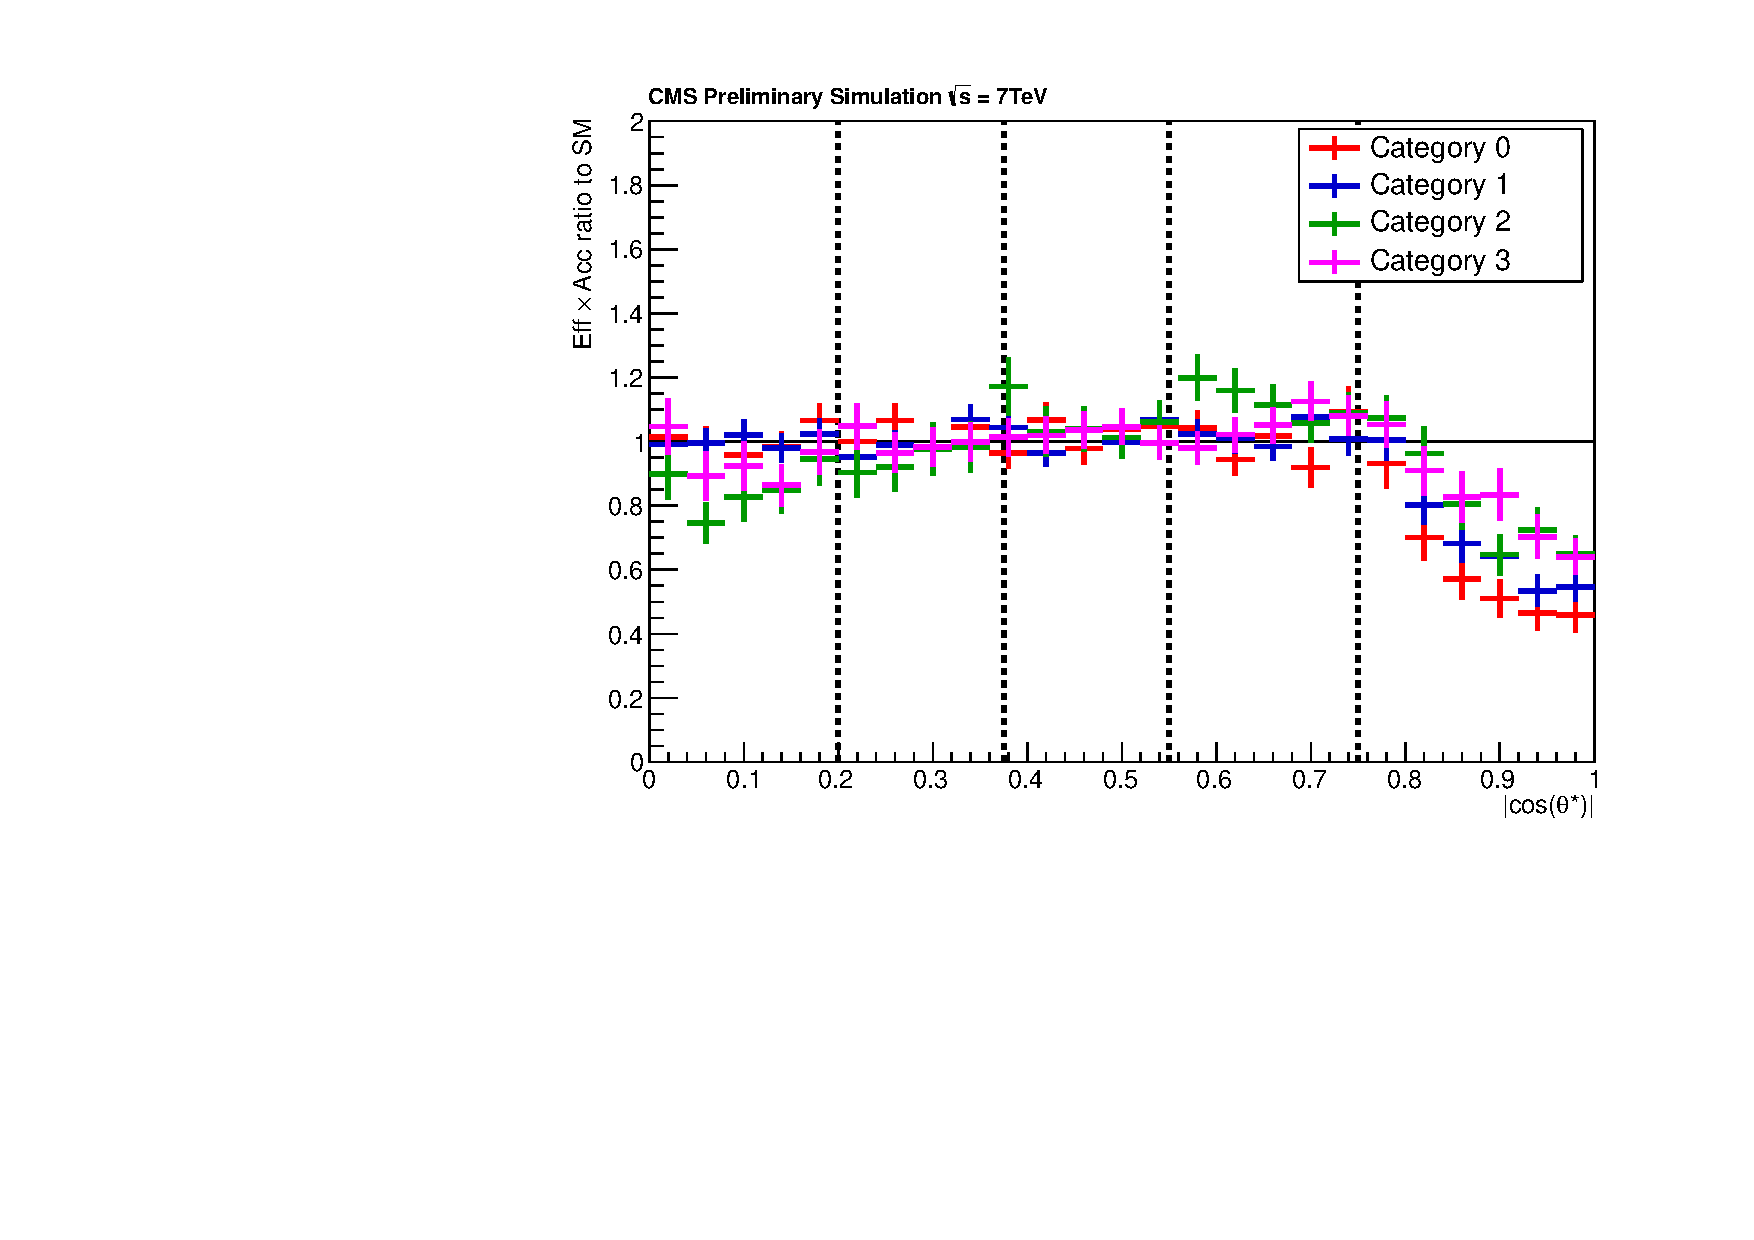
\includegraphics[width=0.49\linewidth]{spin/plots/effacccats_7TeV.pdf}
	\includegraphics[width=0.49\linewidth]{spin/plots/effacccats_8TeV.pdf}
  \caption[Acceptance $\times$ efficiency ratio between the \twomp (gluon fusion production) and \zerop (all SM production modes) of the spin analysis event selection]{Acceptance $\times$ efficiency ratio between the \twomp (gluon-fusion production) and \zerop (all SM production modes) of the event selection as a function of \abscostheta split into the $|\eta|$ and $R_{9}$ categories defined in Table.~\ref{table:cats1}. The \abscostheta category boundaries are shown as the black dashed lines. The left hand plot is for the 7~\TeV \MC and the right hand plot for the 8~\TeV.}
	\label{fig:eff_acc}
	\end{center}
\end{figure}	


To benefit from the improved energy resolution of non-showering photons in 
the barrel, each event is categorised in $\eta$ and $R_{9}$ according to Table~\ref{table:cats1}.

\begin{table}
  \begin{center}
    \begin{tabular}{| l | l l l |}
      \hline
      Category 0 & $|\eta|_{\mbox{\tiny{max}}}<1.5$ & and & $R_{9\mbox{\tiny{min}}}>0.94$ \tabularnewline 
      Category 1 & $|\eta|_{\mbox{\tiny{max}}}<1.5$ & and & $R_{9\mbox{\tiny{min}}}\leq0.94$ \tabularnewline 
      Category 2 & $|\eta|_{\mbox{\tiny{max}}}>1.5$ & and & $R_{9\mbox{\tiny{min}}}>0.94$ \tabularnewline 
      Category 3 & $|\eta|_{\mbox{\tiny{max}}}>1.5$ & and & $R_{9\mbox{\tiny{min}}}\leq0.94$ \tabularnewline
      \hline
    \end{tabular}
    \caption{Definition of photon resolution categories}
    \label{table:cats1}
  \end{center}
\end{table}

%\begin{tabular}{l l l l l}
%  \textbullet & Category 0: & $|\eta|_{\mbox{\tiny{max}}}<1.444$ & and & $R_{9\mbox{\tiny{min}}}>0.94$ \\ 
%  \textbullet & Category 1: & $|\eta|_{\mbox{\tiny{max}}}<1.444$ & and & $R_{9\mbox{\tiny{min}}}\leq0.94$ \\ 
%  \textbullet & Category 2: & $|\eta|_{\mbox{\tiny{max}}}>1.444$ & and & $R_{9\mbox{\tiny{min}}}>0.94$ \\ 
%  \textbullet & Category 3: & $|\eta|_{\mbox{\tiny{max}}}>1.444$ & and & $R_{9\mbox{\tiny{min}}}\leq0.94$ \\
%\end{tabular}

Within each category events are binned in \abscostheta, to discrimate between the different spin hypotheses, according to Table.~\ref{table:cats2}.

\begin{table}
  \begin{center}
    \begin{tabular}{| l | r l |}
      \hline
      Spin Category 0 &             & \abscostheta $<0.2$ \tabularnewline 
      Spin Category 1 & $0.2\leq$   & \abscostheta$<0.375$ \tabularnewline 
      Spin Category 2 & $0.375\leq$ & \abscostheta$<0.55$ \tabularnewline 
      Spin Category 3 & $0.55\leq$  & \abscostheta$<0.75$ \tabularnewline 
      Spin Category 4 & $0.75\leq$  & \abscostheta$<1.0$ \tabularnewline 
      \hline
    \end{tabular}
    \caption{Definition of photon \abscostheta categories}
    \label{table:cats2}
  \end{center}
\end{table}


The \abscostheta boundaries are optimised to make particular use of the most disciminating 
bin (high \abscostheta) and to maintain uniform acceptance $\times$ efficiency in the 
other bins. In total the analysis is split into 20 event classes (4 $\eta$/\rnine\xspace 
categories $\times$ 5 \abscostheta categories) in each year which gives a total of 40 event classes.

\subsection{Signal and Background modelling}

The signal models are obtained from \MC simulation as described in Sec.~\ref{sec:mc} for the spin-0 \SM processes and the spin-2 processes. A parametric model identical to the one built for the nominal analysis is constructed as per the method described in Sec.~\ref{sec:signal_mfm}. The signal model is then parametrised as before in terms of $\mu$, \mH and two additional parameters, $x$ and \fqqbar, which dictate the amount of signal from spin-2 and the amount of spin-2 from $q\bar{q}$ production. The signal model parametrisation can be written as,
\begin{equation}
  \textbf{S}(m_{H},fqq,x;\hat{\theta}) = (1-x)\cdot\boldsymbol{S_{SM}}(m_{H};\hat{\theta})  + x\cdot\Bigl[f_{q\bar{q}}\cdot \boldsymbol{S_{q\bar{q}}}(m_{H};\hat{\theta}) + (1-f_{q\bar{q}})\boldsymbol{S_{gg}}(m_{H};\hat{\theta})\Bigr],  
  \label{eq:spin_sig}
\end{equation}
where $x$ is the amount of signal originating from spin-2, \fqqbar is the amount of spin-2 signal originating from $q\bar{q}$ production, \mH is the signal position and $\theta$ are the nuisance parameters.

The background model for the spin analysis comes in two forms. For the differntial measurement of the signal strength in bins of \abscostheta the envelope background method is used as per the description in Sec.~\ref{sec:envelope}. However, when calculating the statistical separation between various spin hypotheses a single parametrisation of the background is used in each category, namely a polynomial in the Bernstein basis~\cite{bernsteins1,bernsteins2} as per the description in eq.~\ref{eq:bernsteins}. The reason for this is that there is no asymptotic approximation for the test statistic distribution when the null hypothesis is not embedded in the alternative hypothesis. Consequently, in order to obtain the test statistic distributions (like the ones shown in Fig.~\ref{fig:cls}) one has to generate lots of pseudo-data and then refit this data to obtain the likelihood ratio and hence test statistic value. Given the complexity of the spin signal model and the combinatorics involved when using the envelope method with 40 analysis categories this becomes CPU impractical. It has been trialled using the GRID computing network but was found to take the order of hundreds of CPU years.
Given this complication, and the fact that small losses in sensitivity to the background normalisation have a small impact on the spin hypothesis separation power, a single parametrisation in each category was chosen for ease and simplicity. The choice is to use 4th order Bernstein polynomials in all categories apart from the highest \abscostheta categories in which a 3rd order was chosen. The motivation behind this choice is that these order of polynomials show a similarly small level of bias as the envelope method when tested against ``truth" models for the spin categories analogous to the description in Sec.~\ref{sec:envelope}.

